% ------------------------------------------------------------------------
%
% -------------------      Plantilla_UIS.tex       -----------------------
%               ESTE ES EL MAIN.TEX ESTE ARCHIVO LLAMA A TODOS LOS ARCHIVOS QUE COMPONEN LA TESIS....
% ------------------------------------------------------------------------
% ------------------------------------------------------------------------
% ------------------------------------------------------------------------
% Versión de plantilla para realización de informes de trabajo de grado
% construida para uso de la Universidad Industrial de Santander.
%
% Reservados todos los derechos
%
% Bucaramanga, Colombia
%
% Febrero 03 de 2019
%
% ------------------------------------------------------------------------
% ------------------------------------------------------------------------
% ------------------------------------------------------------------------
%
% ------------------------------------------------------------------------
\documentclass[letter,oneside,12pt,spanish]{report}          % Encabezados
% ------------------------------------------------------------------------
\usepackage{uislatexstyleAPA}                           % Libreria UIS APA
%------------------------------
% ------------------------------------------------------------------------
% Ingrese en este punto las librerías específicas de usuario
% ------------------------------------------------------------------------
\usepackage{epsfig}
\usepackage{amsmath}
\usepackage{amssymb}
\usepackage{subfigure}
%Image-related packages
\usepackage{graphicx}
%\usepackage{subcaption}
\usepackage[export]{adjustbox}
\usepackage{wrapfig}
\usepackage{float}
\usepackage{comment}
\usepackage{pdflscape}
\usepackage{booktabs}
\usepackage{pdflscape}
\usepackage{longtable}
\usepackage{siunitx}
\usepackage[acronym]{glossaries}
\makeglossaries
\setacronymstyle{long-short-desc}

% ------------------------- NUEVO-----------------------------------------------
\bibliography{bib_jgrisales.bib}
% ------------------------------------------------------------------------
\begin{document}                                     % Inicio de documento
% ------------------------------------------------------------------------
% Definición silábica de palabras
% ------------------------------------------------------------------------
%\hyphenation{pro-por-cio-nal di-se-ño}
% ------------------------------------------------------------------------
% Titulo resumido del trabajo que aparecerá en cornisa
% ------------------------------------------------------------------------
%\title{Estudio de los efectos de la actividad solar a largo plazo sobre el flujo de rayos cósmicos secundarios en el observatorio Pierre Auger.}
\title{}
% ------------------------------------------------------------------------
% Elementos previos al contenido del trabajo
% ------------------------------------------------------------------------
% ------------------------------------------------------------------------
%                               Portadilla
% ------------------------------------------------------------------------

\begin{center}

Estudio de los efectos de la actividad solar a largo plazo sobre el flujo de rayos cósmicos secundarios en el observatorio Pierre Auger \vspace{1.5cm}

Jennifer Grisales Casadiegos\\ \vspace{1.5cm}

Trabajo de Grado para optar al título de Magíster en Física\\ \vspace{0.5cm}

Director\\
Luis A. Núñez\\
PhD en Ciencias\\ \vspace{1cm}
Co-Director\\
Roberto Mussa\\
PhD en Ciencias \vspace{1.5cm}

Universidad Industrial de Santander\\
Facultad de Ciencias\\
Escuela de Física\\
Bucaramanga\\
2023\\

\end{center}
\begin{comment}
    % ------------------------------------------------------------------------
%                             Nota de proyecto
% ------------------------------------------------------------------------

\newpage

\begin{figure}[htb!]
\centering
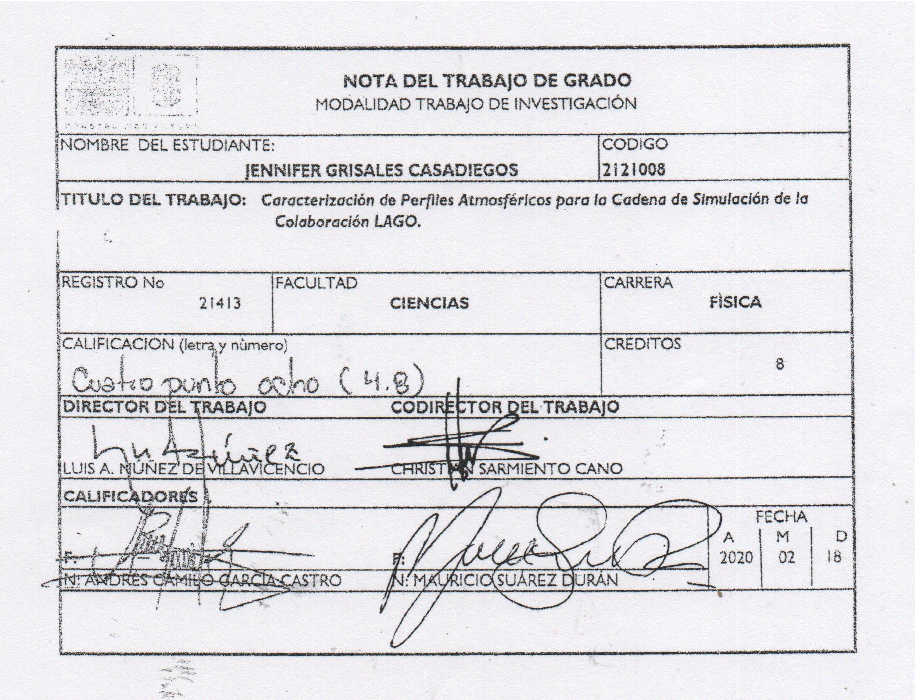
\includegraphics[width=1.0\textwidth]{Secs/NOTA_TESIS.pdf}
\end{figure}

% ------------------------------------------------------------------------
%                             Autorización
% ------------------------------------------------------------------------

\newpage


\begin{figure}[htb!]
\centering
\includegraphics[width=1\textwidth]{Secs/Carta_AUTORIZACIÓN.pdf}
\end{figure}

% ------------------------------------------------------------------------ 

\end{comment}
             % Portadilla, formato de nota y autorización
% ------------------------------------------------------------------------
%% \addcontentsline{toc}{chapter}{Dedicatoria}
  
%   \cleardoublepage
\newpage

\vspace*{\stretch{3}}

\begin{flushleft}
\textit{¿En perseguirme, mundo, qué interesas?}\newline
\textit{¿En qué te ofendo, cuando sólo intento}\newline
\textit{poner bellezas en mi entendimiento}\newline
\textit{y no mi entendimiento en las bellezas?}\newline
\textit{Yo no estimo tesoros ni riquezas,}\newline
\textit{y así, siempre me causa más contento}\newline
\textit{poner riquezas en mi entendimiento}\newline
\textit{que no mi entendimiento en las riquezas.}\newline
\textit{Y no estimo hermosura que vencida}\newline
\textit{es despojo civil de las edades}\newline
\textit{ni riqueza me agrada fementida,}\newline
\textit{teniendo por mejor en mis verdades}\newline
\textit{consumir vanidades de la vida}\newline
\textit{que consumir la vida en vanidades.}\newline
\textit{``Quéjase de la suerte" por Juana Inés de Asbaje.}\newline

\textit{Este trabajo va dedicado a todas las mujeres que han defendido nuestro derecho al conocimiento.}
\end{flushleft}



\clearpage                                   % Dedicatoria
% ------------------------------------------------------------------------
%%\addcontentsline{toc}{chapter}{Agradecimientos}
\newpage
\chapter*{Agradecimientos}

Son muchas las personas que, sabiéndolo o no, fueron contribuciones significativas, en una combinación lineal que determinó el camino de mi formación como Física. A todos y todas, gracias. Fuertemente en mis recuerdos mis compañeros de aprendizaje Edwin Florez, Genderson Rueda y Yerson Barragán, con quienes pese a las dificultades, disfrutamos esta etapa universitaria formando no solo nuestro pensamiento científico, sino también construyendo una necesaria conciencia de clase que orientará nuestro quehacer académico y político por siempre. Debo agradecer a mi madre y mi padre, porque debido a su formación, desde mi infancia nació el sueño de vivir la ciencia. Personas como José Quintero que me alentaron a seguir adelante y sacar valentía de donde no había, gracias. También a Jesús Sánchez por abrirme las puertas de su casa, y su familia, gracias por todo el afecto y el apoyo incondicional. A mi mejor amiga Luz Marina Cabrera por ser mi confidente y por jugar conmigo a dibujarnos mutuamente alas para volar y soñar.

Gracias a Luis Núñez por inspirarme siempre y mostrarme que la ciencia es el camino. Gracias Christian Sarmiento por creer en mí y por su tiempo que valoré infinitamente. También gracias a Yeinzon Rodríguez porque me demostró que es posible seguir viendo la física con curiosidad y pasión.

Finalmente quiero agradecer a Jesús Peña haber sido mi apoyo emocional en todo este proceso. Por ser mi ejemplo e inspiración de esfuerzo, perseverancia, trabajo duro y amor genuino por la ciencia. Gracias por tanto amor.                           % Agradecimientos
% ------------------------------------------------------------------------
\tableofcontents                                      % Tabla de contenido
% ------------------------------------------------------------------------
%\listoffigures                         % Lista de figuras, tablas y anexos
%\listoftables
%\listofanexo
% ------------------------------------------------------------------------
%\include{Secs/glosario}                             % Glosario de términos
%\newacronym[description={Rayos Cósmicos, por sus siglas en ingles}]{cr}{CR}{Cosmic Rays (Rayos Cósmicos)}
\newacronym{cr}{CR}{Cosmic Rays (Rayos Cósmicos)}
\newacronym{eas}{EAS}{Extensive Air Showers (Cascadas Aéreas Extensas)}
\newacronym{gcr}{GCR}{Galactic Cosmic Rays (Rayos Cósmicos Galácticos)}
\newacronym{cme}{CME}{Coronal Mass Ejections (Ejecciones de Masa Coronal)}
\newacronym{icme}{ICME}{Interplanetary Coronal Mass Ejections (Ejecciones de Masa Coronal Interplanetarias)}
\newacronym{wcd}{WCD}{Water Cherenkov Detector (Detector Chérenkov de Agua)}
\newacronym[description={Detectores de superficie del Observatorio Pierre Auger}]{sd}{SD}{Surface detector}
\newacronym{fds}{FD}{Fluorescence Detector (Detector de FLuorescencia)}
\newacronym{pmt}{PMT}{Photomultiplier Tube}
\newacronym{FADC}{FADC}{Flash Analog-to-Digital Converter}
\newacronym{grb}{GRB}{Gamma Ray Burst}
\newacronym{cri}{CRI}{Cosmic Ray Intensity}
\newacronym{fd}{FD}{Decrecimiento Forbush}
\newacronym{fe}{FE}{Evento Forbush}




\printglossary[type=\acronymtype,title=Acrónimos]

% ------------------------------------------------------------------------
% Contenido del Informe
% ------------------------------------------------------------------------
%\addcontentsline{toc}{chapter}{RESUMEN}
\newpage
\chapter*{Resumen}
\label{sec:resum}
\footnotesize{
\noindent\textbf{TÍTULO:}  ESTUDIO DE LOS EFECTOS DE ACTIVIDAD SOLAR A LARGO PLAZO
SOBRE EL FLUJO DE RAYOS CÓSMICOS SECUNDARIOS EN EL OBSERVATORIO PIERRE AUGER\astfootnote{Trabajo de grado}

\noindent\textbf{AUTORA:} Jennifer Grisales Casadiegos\asttfootnote{Facultad de Ciencias. Escuela de Física. Director: Luis A. Núñez. }

\noindent\textbf{PALABRAS CLAVES: } Rayos Cósmicos Galácticos, Viento Solar, Ciclo Solar, Decrecimientos Forbush, Detectores Chérenkov.

\noindent \textbf{DESCRIPCIÓN: }

En este trabajo de grado, se presentan los resultados de un estudio centrado en los impactos a largo plazo de la actividad solar sobre el flujo de rayos cósmicos secundarios en el Observatorio Pierre Auger, utilizando el \textit{Modo Scaler}. Este sistema de detección de baja energía registra el flujo de fondo de rayos cósmicos en términos de partículas por segundo, con el propósito de detectar destellos de rayos gamma y eventos transitorios como las disminuciones de Forbush. A pesar de estar optimizado para partículas con energías superiores a $10^{18}eV$, el Observatorio Pierre Auger implementó este sistema para aprovechar las capacidades del arreglo de detectores Chérenkov.

El objetivo principal de esta tesis consiste en analizar la influencia de la actividad solar en la detección de rayos cósmicos galácticos y determinar cómo se puede extraer información pertinente sobre el ciclo solar y el clima espacial a partir de los datos del Observatorio. Para llevar a cabo este propósito, se realizó un análisis exhaustivo de los scaler, desde el año 2006 hasta el 2021 gran parte correspondiente al ciclo solar 24 y se contrastaron con datos provenientes de otros experimentos y fuentes, tales como monitores de neutrones, y satélites en el caso de los datos de manchas solares y el viento solar. El estudio se enfocó en examinar la correlación entre el flujo de rayos cósmicos y los parámetros solares, así como la respuesta del Observatorio a eventos solares transitorios, como erupciones solares y eyecciones de masa coronal. Los resultados revelan que el Observatorio Pierre Auger exhibe sensibilidad a las variaciones del clima espacial tanto a corto como a largo plazo, y puede utilizarse como un instrumento complementario valioso para la investigación de la actividad solar y sus efectos sobre la Tierra.
}\normalsize
\clearpage                                               % Resumen
%%\addcontentsline{toc}{chapter}{Abstract}
\newpage
\chapter*{Abstract}
\label{sec:abst}
\footnotesize{
\noindent\textbf{TITLE:} CHARACTERIZATION OF ATMOSPHERIC PROFILES FOR THE LAGO SIMULATION CHAIN\astfootnote{Bachelor Thesis}

\noindent\textbf{AUTHOR:} Jennifer Grisales Casadiegos.\asttfootnote{Facultad de Ciencias. Escuela de Física. Director: Luis A. Núñez. Codirector: Christian Sarmiento.}

\noindent\textbf{KEYWORDS: } Astroparticle, particle flux, atmosphere, simulation, extensive air shower.

\noindent\textbf{DESCRIPTION:} One of the main objectives of the Space Weather program of the Latin American Giant Observatory (LAGO), is to study the influence of the solar activity on the secondary particle flux  variations, produced during the interaction between astroparticles with atmosphere. To this end, a chain of simulations is carried out, which estimates in detail, the Primary's development, from its entry into the Earth's atmosphere, to the Water Cherenkov Detector response. This work, complete the simulation chain, focusing their interest in to study the atmospheric effect on the secondary particle flux. To do this it developed a methodology that allows the creation and use of monthly atmospheric profiles, for any localization, in the EAS simulations within the CORSIKA code. Furthermore, the relevance to using the new monthly profiles it was checked, because they are able to reproduce in the secondary particle flux, the effect of the temperature changes along the year. This allows refine the estimates made.
}\normalsize
\clearpage                                              % Abstract
% ------------------------------------------------------------------------
% Capítulos
% ------------------------------------------------------------------------
\addcontentsline{toc}{chapter}{Introducción}
\newpage
\chapter*{Introducción}
\label{sec:intro}

\noindent El Sol es la estrella más cercana a la Tierra y la principal fuente de energía para la vida en nuestro planeta. Su actividad se manifiesta en forma de cambios en la luminosidad, campo magnético, viento solar y transporte de partículas, además que lo hace a diferentes ritmos, desde minutos hasta siglos  (\cite{Balogh_2008}). El periodo de actividad más conocido el el ciclo de 11 años que se caracteriza por el aumento y la disminución del número de manchas solares donde se concentra el campo magnético debido al mecanismo de convección de su plasma (\cite{Balogh_2008}).

El estudio exhaustivo de la dinámica solar y todos los fenómenos determinados por la interacción entre el viento solar, el campo magnético interplanetario y el campo magnético terrestre se conoce hoy como \textit{Clima Espacial} (\cite{singh_2021}). El término se empezó a usar en los años 50 y se popularizó en los años 90. Sin embargo, antes de eso ya se habían observado y caracterizado algunos fenómenos de clima espacial como las auroras, las tormentas magnéticas o los rayos cósmicos (\cite{cade_2015}). Por ejemplo, el primer registro de una tormenta magnética fue realizado por el naturalista Alexander von Humboldt en 1808 relacionándola con las manchas solares (\cite{Lakhina_2007}), o el registro en 1859 de la mayor tormenta magnética conocida \textit{el evento Carrington}, que causó auroras espectaculares y daños en las líneas telegráficas (\cite{hayakawa_2019}). En el siglo XX, el desarrollo de la tecnología espacial hizo que el clima espacial fuera más relevante, ya que podía afectar a los satélites, las comunicaciones, la navegación o la salud de los astronautas (\cite{Schrijver_2015}) y se comenzaron a desarrollar instrumentos tanto en el espacio como en la Tierra, que permiten observar el Sol, el viento solar, el campo magnético interplanetario, el campo magnético terrestre, la ionosfera y la atmósfera. 
%(\cite{cade_2015})

Entre estos instrumentos se encuentran los detectores de rayos cósmicos: partículas cargadas que provienen de diversas fuentes astrofísicas incluido el Sol, capaces de acelerar partículas a altas velocidades, abarcando un amplio espectro de energía (\cite{spurio_2015}).  No obstante, es un hecho bien establecido que al aumentar la energía, disminuye el número de partículas que pueden ser detectadas. En este contexto, el Sol y la galaxia se revelan como las fuentes predominantes, generando lo que hoy llamamos \textit{fondo de rayos cósmicos} (\cite{gaisser_2016}). Hasta la fecha, todas las observaciones realizadas han confirmado que los diversos fenómenos solares son la principal causa de alteración en este flujo de fondo, estableciendo así un vínculo directo entre la medición de estas partículas y la actividad solar (\cite{forbush_1954}).

Uno de los experimentos más importantes construidos para la medición indirecta de rayos cósmicos es el Observatorio Pierre Auger que se encuentra en la provincia de Mendoza, Argentina, y tiene como objetivo estudiar partículas de ultra alta energía (UHECR), es decir, aquellas con energías superiores a los $10^{18}eV$ (\cite{AugerGENERAL_2015}). Sin embargo, a partir del 2005 este observatorio implementó un sistema de detección adicional de baja energía denominado \textit{modo scaler} que registra el flujo de fondo en forma de número de partículas por segundo, con el objetivo de observar destellos de rayos gamma y eventos transitorios como Forbush Decreases (\cite{DASSO20121563}). Por lo tanto, este nuevo criterio de almacenamiento de eventos ha abierto un mundo de nuevos análisis e información física que en los últimos años ha logrado mayor interés en la comunidad científica.

La presente tesis de maestría hace parte de este conjunto de trabajos que busca caracterizar al arreglo de detectores de superficie como un sensor de alta resolución del rayos cósmicos galácticos (\cite{DASSO20121563}, \cite{asorey},\cite{masias_2017},\cite{Martin_Schimassek2022}). Mas específicamente, aquí presentamos un estudio de los efectos de la actividad solar a largo plazo sobre el flujo de rayos cósmicos secundarios en el Observatorio Pierre Auger, utilizando el modo Scaler, considerando el efecto que tienen los eventos transitorios en estas mediciones (\cite{roberta_2018}, \cite{Martin_Schimassek2022}). 


Este trabajo se organiza en cuatro apartados principales. El capítulo uno se centra en los rayos cósmicos, su origen, espectro de energías y su propagación a través de la heliósfera, el campo geomagnético y la atmósfera terrestre, haciendo un recorrido por los fenómenos físicos de principal interés. El capítulo dos describe el Observatorio Pierre Auger, sus detectores y la forma como se aprovecha para medir el fondo de rayos cósmicos.

El capítulo tres presenta los resultados del análisis de los datos del modo Scaler del Observatorio Pierre Auger, desde el año 2006 hasta el año 2021, y lo obtenido al compararlos con los datos de otros detectores como monitores de neutrones, satélites. A partir de lo anterior se explora cuantitativamente la correlación entre el flujo de rayos cósmicos y los parámetros solares, así como la respuesta del Observatorio a los eventos solares transitorios, como las erupciones solares y las eyecciones de masa coronal y su afectación al ciclo solar de 11 años. Por último se presentan las conclusiones donde se realiza un recuento detallado de los resultados obtenidos a lo largo de la investigación y se discuten las implicaciones de las observaciones sugiriendo direcciones para estudios futuros.

  %que contiene todos los resultados de la investigación, se concentra en cuantificar los efectos de la modulación del fondo de rayos cósmicos debido a la actividad solar a corto y largo plazo, describiendo los datos e instrumentos utilizados de tal forma que faciliten su reproducibilidad.  se presentan las conclusiones de la tesis. 
  

%%%%%%%%%%%%
   % Introducción
\include{Prelim/Objtivos}   % Objetivos
\newpage
%%%%%%%%%%%%%%%%%%%%%%%%%%%%----->SECCIÓN 2<-----%%%%%%%%%%%%%%%%%%%%%%%%%
\chapter{Rayos cósmicos}
%%%%%%%%%%%%%%%%%% NEWWWW
Los rayos cósmicos (en adelante CR por sus siglas en inglés) son partículas cargadas que viajan a través del espacio intergaláctico a velocidades cercanas a la luz. Estas partículas, que provienen de diversas fuentes, incluyendo el Sol, supernovas, pulsares, agujeros negros entre otras, son en su mayoría protones y núcleos atómicos. Su composición es diversa, con una predominancia de protones $(~89\%)$, seguidos por núcleos de helio $( 10\%)$ y núcleos pesados $( 1\%)$. También pueden estar constituidos por partículas elementales como electrones o fotones de alta energía  (\cite{kampert_2012}).

En este capítulo, nos adentraremos en el estudio de los rayos cósmicos, comenzando con una descripción de su origen y el espectro de energías que presentan. Describiremos en detalle los mecanismos de detección de los rayos cósmicos, proporcionando una visión de cómo estos fenómenos astrofísicos son estudiados en la actualidad.  A continuación, exploraremos cómo se propagan a través de la heliósfera, el campo geomagnético y finalmente la atmósfera terrestre. En cada etapa de su viaje, los rayos cósmicos interactúan con el medio de formas que afectan su propagación y finalmente su detección en la Tierra.

Finalmente describiremos la morfología de las cascadas aéreas extensas producidas en la atmósfera terrestre y las interacciones hadrónicas y electromagnéticas que las generan. Este análisis es esencial, ya que nuestro estudio se centra en la detección en tierra de la componente electromagnética de las cascadas aéreas, especialmente los muones y electrones que llegan al nivel del suelo. Estas partículas subatómicas juegan un papel crucial en nuestra comprensión de los rayos cósmicos y su interacción con la atmósfera terrestre. 

\section{Origen y espectro de energías}

Los rayos cósmicos, que abarcan un amplio espectro energético, son en su mayoría hadrones, partículas subatómicas que incluyen protones y núcleos atómicos. Estos hadrones cubren valores inferiores a $1 GeV$ hasta más allá de $10^{20} eV$.  A baja energía, la detección de estos hadrones está limitada por la existencia de un corte geomagnético, al menos en medidas realizadas cerca de la Tierra (\cite{Riggi_2023}). El flujo de hadrones de baja energía está sujeto a grandes variaciones temporales, tanto periódicas como transitorias, debido a la influencia del Sol. Sin embargo, estas variaciones se vuelven despreciables a medida que aumenta la energía cinética de los primarios.

Para la medición se pueden emplear diferentes métodos, que dependen de la energía de las partículas. Los métodos directos de detección de rayos cósmicos implican el uso de instrumentos enviados al espacio en globos, cohetes o satélites para medir las características de las partículas primarias que llegan a la Tierra. Algunos ejemplos de estos instrumentos incluyen los detectores de trazas nucleares, que muestran las trayectorias de las partículas cargadas; los espectrógrafos magnéticos, que aplican campos magnéticos para desviar las trayectorias de las partículas cargadas; los calorímetros, que calculan la energía que pierden las partículas cargadas \cite{tomassetti_2023}.

Un ejemplo representativo de un instrumento de detección directa es el Espectrómetro Magnético Alfa (AMS) en la Estación Espacial Internacional, que mide los rayos cósmicos de alta energía o el Espectrómetro de Isótopos de Rayos Cósmicos (CRIS) en la nave espacial Advanced Composition Explorer (ACE) (\cite{tomassetti_2023}), que proporciona mediciones de los isótopos de núcleos de rayos cósmicos galácticos que van desde el helio hasta el zinc.

Los métodos indirectos de detección utilizan la atmósfera como un calorímetro y detectan las partículas secundarias que se crean cuando las partículas primarias chocan con la atmósfera. Estas partículas secundarias son más abundantes y más fáciles de detectar que las partículas primarias. Uno de los instrumentos más representativos de detección indirecta es el Observatorio Pierre Auger, que utiliza una técnica de detección híbrida para estudiar los rayos cósmicos de ultra alta energía y sondear las interacciones hadrónicas a energías mucho más allá de las accesibles por los aceleradores de partículas (\cite{engel_2021}) (los detalles se describirán en el capítulo 2).

El espectro energético de los rayos cósmicos, obtenido a través de toda esta variedad de instrumentos y experimentos, muestra tendencias notables como la rodilla, la segunda rodilla y el tobillo, que corresponden a cambios abruptos en la pendiente a un valor de energía específico. Este espectro sigue una ley de potencia, del tipo $E^{-\gamma}$, con el exponente $\gamma$ variando en diferentes regiones energéticas (\cite{Riggi_2023}). Para visualizar mejor la tendencia del espectro, se suelen representar los valores de flujo multiplicados por $E^{\gamma}$, eligiendo un valor adecuado del exponente $\gamma$ (entre 2,5 y 3) como se observa en la figura \ref{fig:spectrum}. Esta representación permite verificar si la tendencia de los datos sigue esta ley, ya que idealmente los valores se dispondrían a lo largo de una línea horizontal.

\begin{figure}
    \centering
    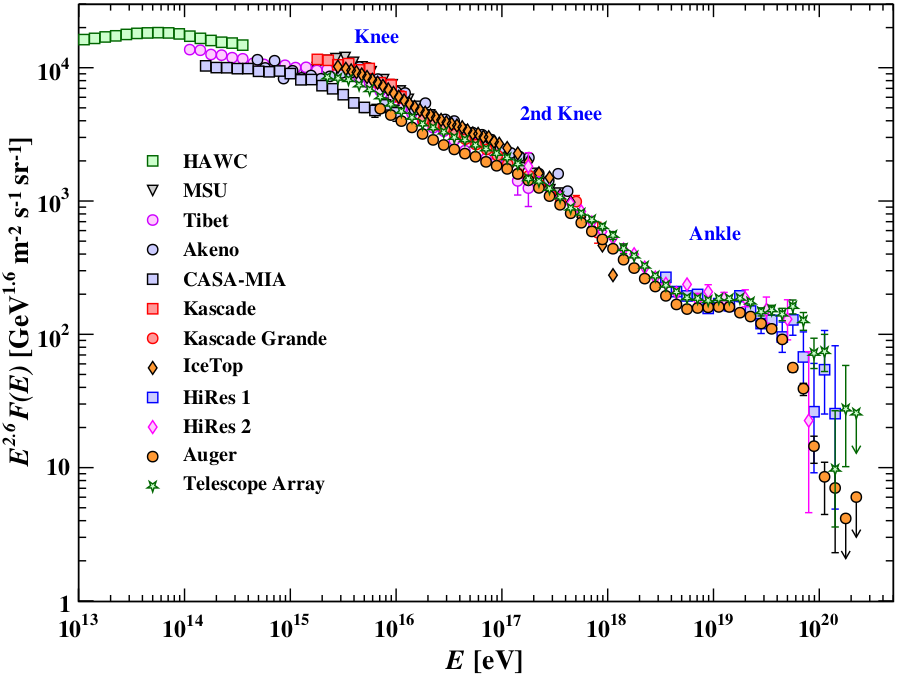
\includegraphics[width=0.8\linewidth]{Figs/CR_spectrum.png}
    \caption{Enter Caption. Fuente \cite{PDG}}
    \label{fig:spectrum}
\end{figure}

%%%%%%  ORIGEN DE LOS RAYOS CÓSMICOS DE ANTES DEL TOBILLO Y DESPUÉS DEL TOBILLO.
%%%% Pierre Cristofari (The transition From Galactic to Extragalactic cosmic rays)
Se tiene evidencia de que los rayos cósmicos (CR) de energías inferiores a la "rodilla" del espectro energético son de origen galáctico. Esto se basa en la observación de los rayos gamma del disco galáctico, que se espera que emitan una señal de rayos gamma mejorada (un incremento en la emisión) debido a la interacción de los CR con el material interestelar (\cite{Cristofari_2023}). Sin embargo, cuando la energía de los CR supera cierto umbral, conocido como el "tobillo", la fuente es de origen extragaláctico (\cite{augerextra}). Esta transición se debe a que los CR de alta energía no pueden confinarse dentro de la galaxia cuando su radio de Larmor es mayor que el tamaño típico del halo galáctico.

\section{Propagación de CR a través de la heliósfera}

El Sol, debido a su proximidad y características, se ha convertido en un laboratorio esencial para la comprensión de la física estelar y es fundamental para la investigación en física del plasma y astrofísica (\cite{Rozelot_2006}). %%%%%ROZELOT

\begin{figure}
    \centering
    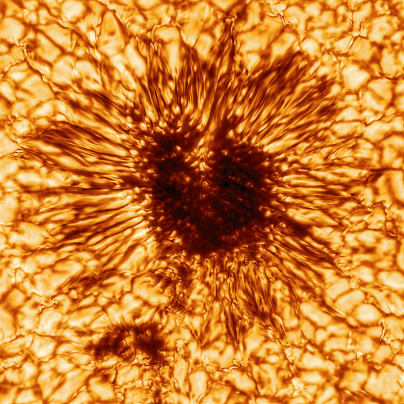
\includegraphics[width=0.6\linewidth]{Figs/sunspot_small.png}
    \caption{La cámara Inouye Solar Wave Front Correction (WFC) de la NSF capturó su primera imagen de una mancha solar el 28 de enero de 2020. La imagen revela un corte de la estructura tridimensional de la mancha solar, que se forma por la convergencia de campos magnéticos intensos y gas caliente que burbujea desde abajo. Aunque la imagen presenta una paleta de colores cálidos con tonos rojos y naranjas, fue tomada por el visor contextual de la Cámara de Campo Amplio del Telescopio Solar Inouye a una longitud de onda de 530 nanómetros, que corresponde a la parte amarillo verdosa del espectro visible. Crédito: NSO/AURA/NSF}
    \label{fig:sunspotNSO}
\end{figure}

 %aunque considerado una estrella común
Todos los estudios del Sol hasta la fecha han revelado la sorprendente diversidad de su campo magnético, que se concentra en pequeños tubos de flujo magnético de alta intensidad que emergen desde el interior del Sol y causan estructuras magnéticas retorcidas en la corona (\cite{schrijver_2009}). Adicionalmente, se ha obtenido información muy detallada sobre su estructura interna: delimitada por distintas capas, cada una de ellas fundamental en la generación y difusión de su energía. La zona interna del Sol, que incluye el núcleo y la zona radiativa, abarca aproximadamente el $85\%$ del radio total. El núcleo, que es donde ocurre la fusión nuclear, se encuentra dentro del $20\%$ del radio solar y contiene el $34\%$ de la masa del Sol. Por encima del núcleo, la zona radiativa se extiende desde aproximadamente el $25\%$ hasta el $70\%$ del radio solar. Por lo tanto, la mayor parte del Sol está compuesta por su zona interna (\cite{Hanslmeier_2023}). 

El  casi$~30\%$ restante le corresponde a la zona convectiva. En esta zona, el Sol no es lo suficientemente caliente para transferir energía por radiación térmica. En esta capa Sol presenta una estructura conocida como granulación, para transportar energía desde el borde de la zona radiativa hasta la superficie. A medida que el plasma se eleva, libera calor al llegar a la superficie solar. Luego, al enfriarse, desciende, perpetuando un ciclo continuo de transporte de energía. Este proceso genera campos magnéticos a través de un mecanismo conocido como 'mecanismo de dínamo solar (\cite{Sturrock_1986}).

La atmósfera del Sol, que incluye la fotosfera, la cromosfera y la corona, juega un papel crucial en la actividad solar. Aunque estas capas representan una pequeña fracción del radio total del Sol ($0.43\%$), son el escenario de varios fenómenos que definen la actividad solar. La fotosfera, que es la capa que vemos desde la Tierra y tiene un grosor de aproximadamente 500 km, es donde se manifiestan las manchas solares, que son indicadores de la actividad magnética del Sol y su mecanismo de convección. La cromosfera, con un grosor de aproximadamente 2500 km, es el lugar donde ocurren las fulguraciones solares, que son explosiones de energía causadas por el reajuste de las líneas del campo magnético. La corona solar, aunque se extiende mucho más allá de la cromosfera, es notablemente menos densa y es la fuente del viento solar (\cite{Rozelot_2006}). Estos fenómenos están intrínsecamente vinculados al campo magnético del Sol, que parece ser el principal impulsor de las actividades solares (\cite{Sturrock_1986}). Así, aunque la atmósfera del Sol representa solo una pequeña fracción de su radio total, su influencia se extiende mucho más allá, afectando no solo al clima espacial, sino también a nuestra vida diaria en la Tierra.

Más allá de la los límites de lo que se puede denominar corona solar, se extiende la heliósfera: una región extensa dominada por el Sol, caracterizada por el viento solar y el campo magnético solar. Esta región protege nuestro sistema solar de la mayoría de los rayos cósmicos galácticos y de los vientos interestelares. El límite de la heliosfera, conocido como heliopausa, se forma cuando el viento solar interactúa con el medio interestelar (\cite{schrijver_2009}). Esta interacción resulta en una compleja dinámica de campos magnéticos y partículas energéticas. El estudio de la heliosfera es esencial para entender el entorno cósmico que nuestro sistema solar atraviesa y para ampliar nuestro conocimiento de otros procesos astrofísicos.

El viento solar, compuesto principalmente por electrones y protones, se origina en la corona solar y se expande hacia el exterior a velocidades de entre 300 y 800 kilómetros por segundo. Este flujo arrastra el campo magnético del Sol, formando una estructura helicoidal conocida como espiral Parker (\cite{Rozelot_2006}). Las fluctuaciones en la velocidad y densidad del viento solar afectan al campo magnético interplanetario y contribuyen a los fenómenos de meteorología espacial (\cite{Rozelot_2006}). El estudio del viento solar es esencial para entender la interacción entre el Sol y su entorno cósmico, y para arrojar luz sobre los procesos que rigen la morfología de la heliosfera.
%%%%%%%%%%%
Las sondas espaciales dan la oportunidad de medir directamente parámetros físicos fundamentales del viento solar. El viento solar no es un fluido estacionario: continuas fluctuaciones del campo magnético son producidas por movimientos turbulentos del gas en el Sol, y escapan hacia el medio interplanetario. Discontinuidades en el campo magnético y ondas de choque se producen por la colisión de viento solar lento y viento solar rápido y por erupciones en la corona solar, eyecciones de masa coronal (CME) y fulguraciones. Las CMEs se propagan a través del sistema solar, y pueden ser medidas cerca de la Tierra como eyecciones de masa coronal interplanetarias (ICMEs). Cuando son suficientemente rápidas generan una onda de choque delante de ellas como se observa en la figura \ref{icme}.

La figura \ref{CME_2003} muestra un ejemplo de una fulguración intensa y una CME, que perturban considerablemente la Heliosfera. Las imágenes fueron tomadas por diferentes instrumentos a bordo de la nave SOHO (ESA/NASA) el 28 de octubre de 2003  y la CME alcanzó la Tierra un día más tarde: grupos de manchas (arriba a la izquierda) indican intensa actividad y complejas estructuras magnéticas en la superficie solar. En la mayor y más compleja de esas regiones aparecieron brillantes fulguraciones. Fue observado, por ejemplo, por el telescopio de ultravioleta extremo (EIT; arriba a la derecha de la figura). Una CME rápida y grande fue observada unos minutos más tarde por el coronógrafo LASCO (al fondo de la figura), propagándose por la corona a una velocidad de 1000 km/s.

\begin{figure}[H]
    \centering
    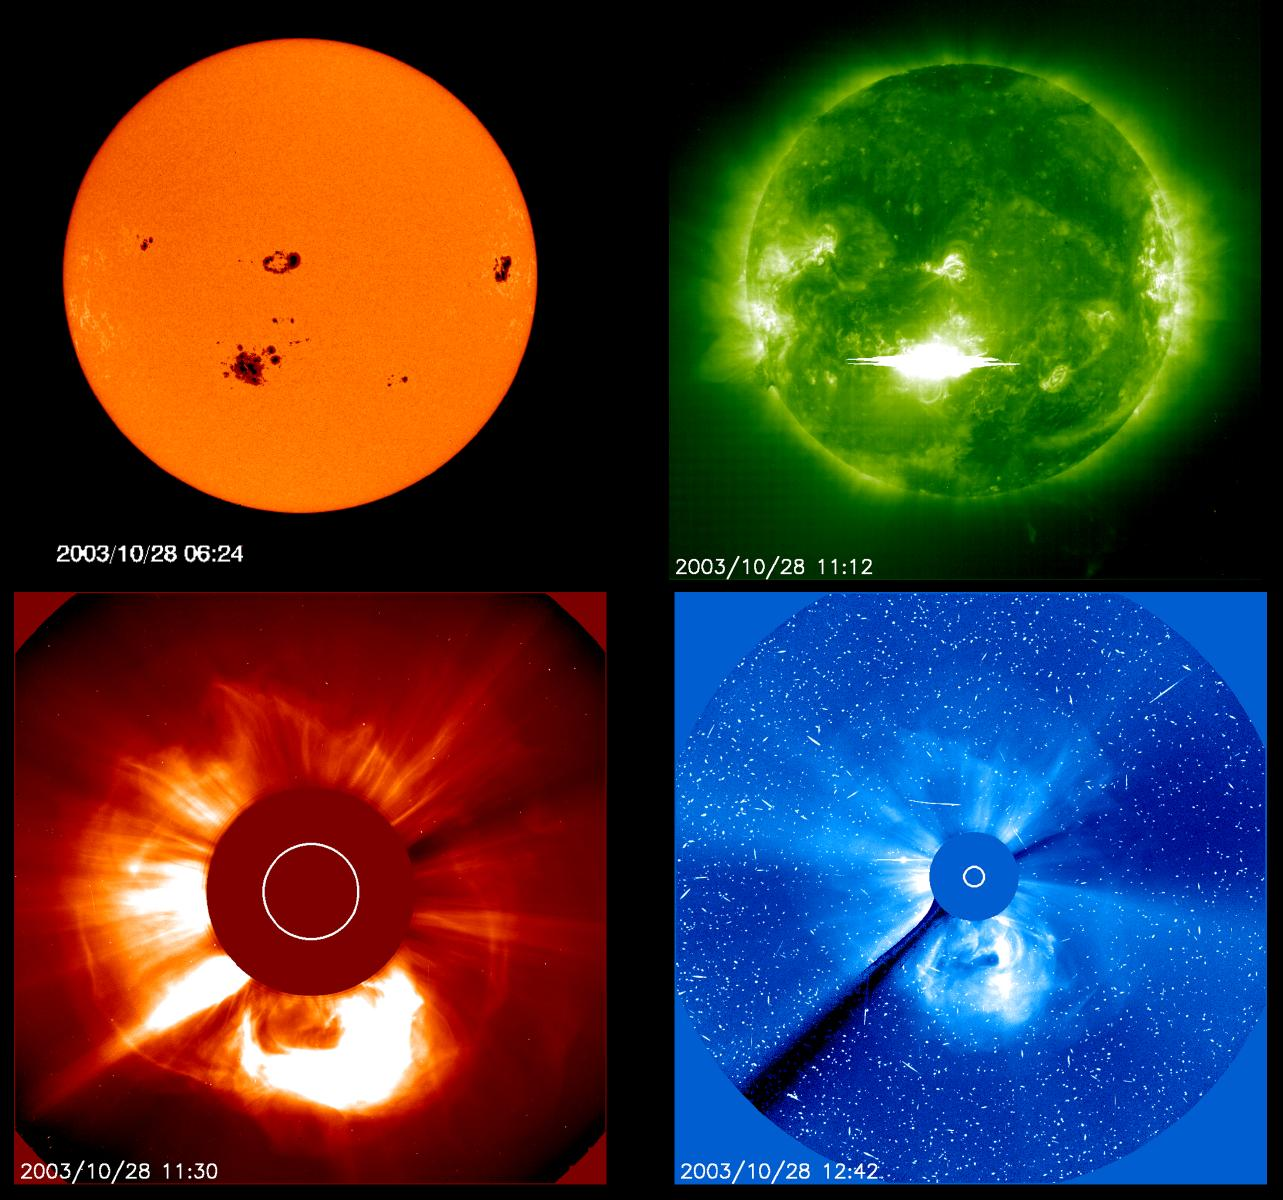
\includegraphics[width=0.6\linewidth]{Figs/flare_2003-10-28.jpg}
    \caption{Enter Caption. Fuente SOHO/MDI, SOHO/EIT, SOHO/LASCO (ESA/NASA)}
    \label{CME_2003}
\end{figure}

La figura \ref{imce} ilustra esquemáticamente este fenómeno: la estructura magnética expulsada desde la corona (línea roja) perturba el campo magnético heliosférico (líneas azules). El viento solar no puede penetrar en la ICME, por lo que se comprime junto con el campo magnético, o se desvía alrededor de la ICME, como indican las dos flechas azules. La configuración de las líneas de campo cambia. En la interfaz entre la ICME y el viento solar circundante, el campo magnético se vuelve turbulento. En esta heliosfera perturbada, tanto los rayos cósmicos solares como los galácticos experimentan condiciones de propagación muy diferentes a las de la heliósfera en estado tranquilo (\cite{NMDB}).

\begin{figure}[H]
    \centering
    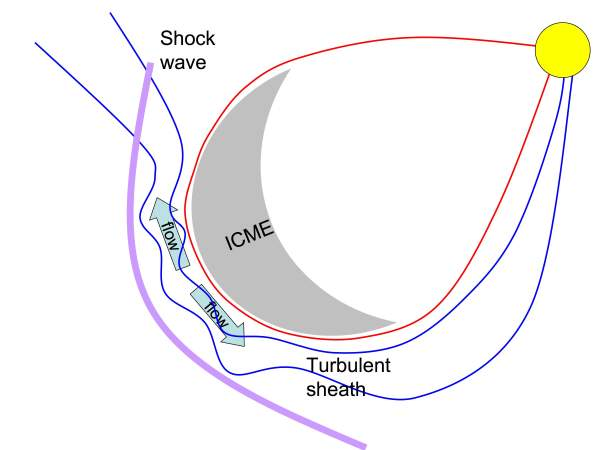
\includegraphics[width=0.5\linewidth]{Figs/Dessin_ICME_sm_0.jpg}
    \caption{Enter Caption. Fuente \cite{NMDB}}
    \label{imce}
\end{figure}
Cuando los rayos cósmicos galácticos llegan a la heliósfera, interactúan con el viento solar que afecta de diferente manera a los rayos cósmicos según su energía. Los que tienen una energía muy alta, $>10GeV$,  tienen una trayectoria rectilínea, ya que la fuerza de Lorentz que ejerce el campo magnético es despreciable en comparación con su momento lineal. Las partículas de energía moderada, de unos pocos $GeV$, tienen una trayectoria difusiva. La difusión se produce por la presencia de irregularidades en el campo magnético del viento solar, que provocan cambios en la dirección e intensidad del campo a lo largo de la trayectoria de las partículas. Estos cambios se deben a la turbulencia del plasma, que genera fluctuaciones en el campo magnético a diferentes escalas espaciales y temporales. La difusión de los rayos cósmicos de energía moderada implica una pérdida de información sobre su dirección de origen y una modulación de su flujo en función del ciclo solar.
%%%%%%%%% NEW

El ciclo solar es el periodo de 11 años en el que la actividad solar varía de forma periódica. Esto se manifiesta en el conteo de manchas solares. El número de manchas solares se correlaciona inversamente con el flujo de rayos cósmicos galácticos medido por la red de monitores de neutrones en la Tierra (más detalles en el capítulo 3). Esto se debe a que cuando el número de manchas solares es alto, el viento solar es más fuerte y el campo magnético interplanetario es más turbulento, lo que dispersa más a los rayos cósmicos galácticos y reduce su flujo. Por el contrario, cuando el número de manchas solares es bajo, el viento solar es más débil y el campo magnético interplanetario es más regular, lo que dispersa menos a los rayos cósmicos galácticos y aumenta su flujo.

Además de la modulación de 11 años, los rayos cósmicos galácticos también presentan variaciones de menor amplitud y duración, relacionadas con la rotación solar de 27 días y con la localización de las regiones activas en el Sol. Estas variaciones se deben a que el viento solar y el campo magnético interplanetario no son homogéneos ni isotrópicos, sino que dependen de la latitud y la longitud solar. Así, los rayos cósmicos galácticos experimentan cambios en su flujo, su espectro de energía y su anisotropía, que es la distribución angular de su intensidad.

Otro aspecto importante del ciclo solar es que cada 11 años el campo magnético solar invierte su polaridad, lo que implica que el ciclo completo es de 22 años. Esto afecta a la propagación de los rayos cósmicos galácticos en la Heliósfera, ya que el campo magnético interplanetario tiene una configuración diferente según la polaridad del campo magnético solar. De esta forma, el flujo de rayos cósmicos galácticos tiene una forma distinta en dos ciclos solares consecutivos. En uno, el flujo tiene un pico pronunciado, con un máximo claro, mientras que en el otro, el flujo tiene una forma más plana, con un máximo menos definido. Escalas superiores al ciclo solar de 11 años quedan por fuera de los alcances de este trabajo.

\textbf{Decrecimientos Forbush}:  La modulación de los rayos cósmicos por el viento solar se ve afectada por la presencia de ICMEs, que son estructuras complejas y dinámicas de plasma y campo magnético que se originan en el Sol y que se propagan por la Heliosfera. La figura \ref{forbush}  muestra este fenómeno  registrado en mayo de 2005 por el observatorio Pierre Auger y el monitor de neutrones de Los Cerrillos (Chile).  Se observa que el flujo de rayos cósmicos disminuye hasta un 20\% durante el paso de una ICME. Estos eventos se denominan decrementos de Forbush, en honor al físico de rayos cósmicos Scott Forbush, que los descubrió en 1937.

\begin{figure}[H]
    \centering
    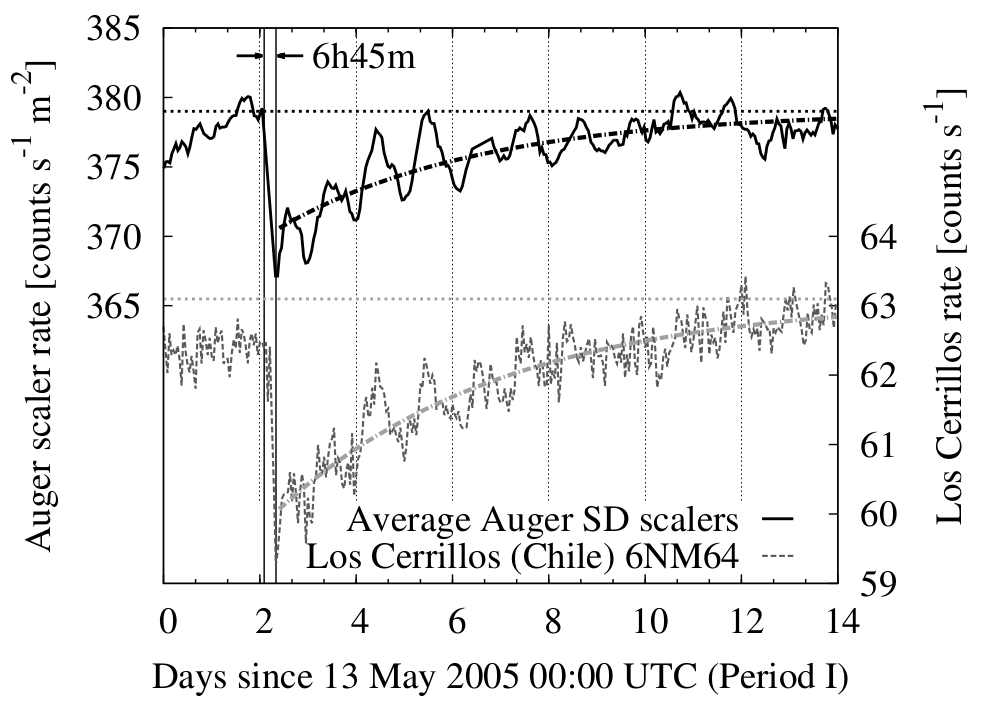
\includegraphics[width=0.6\linewidth]{Figs/mauro_forbush.png}
    \caption{Enter Caption. Fuente \cite{asorey}}
    \label{forbush}
\end{figure}

La disminución del flujo de rayos cósmicos se debe al efecto de apantallamiento que produce la estructura magnética de la ICME y la onda de choque que la acompaña (figura \ref{imce}). El campo magnético de la ICME es más intenso y turbulento que el del viento solar, lo que dispersa más a los rayos cósmicos y los desvía de su trayectoria original. Además, la onda de choque de la ICME comprime el plasma y el campo magnético, lo que crea una barrera que dificulta el paso de los rayos cósmicos. Estos efectos son más notorios para las partículas de menor energía, que son más sensibles a la fuerza de Lorentz que ejerce el campo magnético. Así, los rayos cósmicos que atraviesan una ICME sufren una modulación de su flujo, su espectro de energía y su anisotropía.

\section{Propagación de CR a través del Campo Geomagnético}

Al llegar al entorno terrestre, los rayos cósmicos galácticos se ven afectados por el campo magnético terrestre y la atmósfera. El campo magnético terrestre modula el flujo de los rayos cósmicos galácticos, que depende de su energía y de su dirección de llegada. Los rayos cósmicos galácticos de baja energía son más sensibles a la fuerza de Lorentz que ejerce el campo magnético y pueden ser desviados o excluidos de la magnetosfera. Los rayos cósmicos galácticos de alta energía pueden penetrar la magnetosfera y llegar a la atmósfera.

La Tierra tiene un campo magnético generado por las corrientes eléctricas de su núcleo, que tiene una forma aproximada de un dipolo, con dos polos magnéticos cerca de los polos geográficos. El campo magnético terrestre no está aislado, sino que interactúa con el viento solar, que es el plasma que sale del Sol y que tiene un campo magnético. El viento solar comprime el campo magnético terrestre en la dirección del Sol y lo estira en la dirección opuesta, creando una cola magnética. El campo magnético terrestre forma un sistema casi cerrado de líneas de campo, que delimitan una región del espacio donde el campo magnético terrestre domina sobre el campo magnético interplanetario. Esta región se llama magnetosfera y tiene una forma asimétrica, como se muestra en la figura [1]. La magnetosfera protege a la Tierra de la radiación solar y de los rayos cósmicos galácticos de baja energía, pero también permite la entrada de partículas cargadas que producen fenómenos como las auroras.


\section{Propagación de CR a través de la atmósfera terrestre}

Cuando los CR primarios llegan a la atmósfera terrestre, chocan con los átomos del aire y producen una lluvia de partículas secundarias, que tienen menos energía que el primario. Algunas de estas partículas pueden decaer o interactuar nuevamente con el aire, generando más partículas secundarias. Este proceso se repite varias veces hasta que la energía del primario se disipa o se alcanza el nivel del suelo. A este fenómeno se le llama cascada aérea extensa (en adelante EAS, por sus siglas en inglés).

El estudio de las EAS es fundamental para entender el origen, la naturaleza y la distribución de los CR. Sin embargo, la detección directa se puede realizar hasta el rango de aproximadamente $10^{15}eV$. Como son absorbidos por la atmósfera, deben medirse mediante globos, cohetes o satélites con los que se puede determinar la energía, la composición de la partícula y la dirección de incidencia. Para energías mayores a $10^{15}$ eV, la detección se hace primordialmente de forma indirecta debido a que se reduce significativamente el número de partículas que arriban a la Tierra como se muestra en la figura (\ref{fig:spectrum}). Para tal fin se utilizan detectores a nivel del suelo que registran las señales que dejan las partículas secundarias de las EAS. Estos detectores pueden medir la intensidad, la dirección, la composición y la energía de las EAS, y a partir de ahí inferir las propiedades de los CR primarios \cite{kampert_2012}. 

Para analizar las EAS, se necesita conocer cómo interactúan las partículas con la atmósfera. Un parámetro importante es la profundidad atmosférica $X$ (\ref{eq:eq2}), que mide la cantidad de materia que atraviesa una partícula primaria en su camino por la atmósfera. La profundidad atmosférica depende de la altura $h$ sobre el nivel del mar y de la densidad del aire $\rho(h)$.  
\begin{equation}
X_{v}= \int_{h}^{\infty} \rho (h') dh'.
\label{eq:eq2}
\end{equation}
Por otra parte, teniendo en cuenta la naturaleza de las partículas secundarias, se pueden identificar tres componentes principales: la componente electromagnética, que está conformada por electrones, positrones y fotones; la componente hadrónica, constituida de piones, kaones y bariones, y la componente muónica, generada por el decaimiento de piones y kaones cargados. La figura \ref{fig:fig3} ilustra los procesos de interacción mostrados anteriormente y cómo éstos generan cada una de las componentes. Estas tres componentes se generan debido a interacciones electromagnéticas y hadrónicas en el proceso de penetración a través de la atmósfera que describiremos con un poco más de detalle a continuación.

\begin{figure}[htb!]
\centering
    \begin{center}
        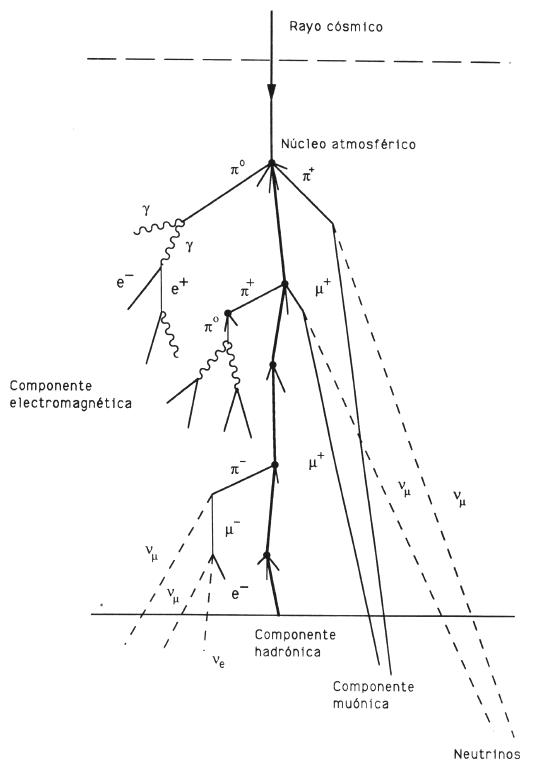
\includegraphics[width=0.5\textwidth]{Figs/componentes_cas.jpg}
    \end{center}{}
    \caption[Esquema del desarrollo de una EAS iniciada por un hadrón.]{Esquema del desarrollo más probable de una EAS iniciada por un hadrón \cite{mauro:tesis}. En la figura se observa el decaimiento del hadrón en piones cargados y neutros, y estos a su vez, al decaer, generan fotones, electrones y muones. Se identifican tres componentes: electromagnética, muónica y hadrónica.}
    \label{fig:fig3}
\end{figure}

\subsection{Interacciones electromagnéticas}
Están presentes cuando el primario incidente es un fotón o un electrón, los principales canales de interacción son la producción de pares y radiación de frenado. Estas partículas pueden crear o emitir otras partículas del mismo tipo al interactuar con los átomos del aire. Los fotones pueden crear pares de electrones y positrones, y estos pueden emitir más fotones al frenarse (bremsstranhlung). Este proceso se detiene cuando los fotones tienen una energía de 1.02 MeV. Para un núcleo de aire con carga $Z$ y número atómico $A$, los procesos de producción son:
\begin{equation}
\begin{split}
&Bremsstrahlung\quad e \quad \xrightarrow{Y^{A}_{Z}} \quad e\gamma ,  \quad y \\
&Pares \quad \gamma \xrightarrow{Y^{A}_{Z}} \quad e^{+}e^{-} \\
\end{split}
\end{equation} 

Otros procesos electromagnéticos que influyen en esta pérdida de energía y deben ser considerados son la\textbf{pérdida de energía por Ionización} de una partícula cargada que atraviesa la materia con un espesor $\lambda$ que es descrita por la ecuación de Bethe-Bloch:
\begin{equation}
dE_{i} = \frac{\lambda \gamma^{2}z^{2}}{\gamma^{2}-1}\kappa_{1}(ln(\gamma^{2}-1)- \beta^{2}+\kappa_{2})
\label{eq:eq20}
\end{equation}

Donde $\beta = v/c $ es la velocidad de la partícula en unidades de la velocidad de la luz, $\gamma$ es el factor de Lorentz, $z$ es la carga de la partícula ionizada en unidades de $e$. Las dos constantes $\kappa_{1}= 0.153287 MeV g^{-1}$ y $\kappa_{2}= 9.386417 MeV g^{-1}$ son los valores correspondientes para el aire \cite{Heck1998}. Esta expresión es usada para calcular la perdida por energía de ionización a través de la trayectoria de la partícula. Por ejemplo, la pérdida de energía de muones como función de su energía está representado en la figura \ref{fig:fig4}.\\

\begin{figure}[htb!]
\centering
        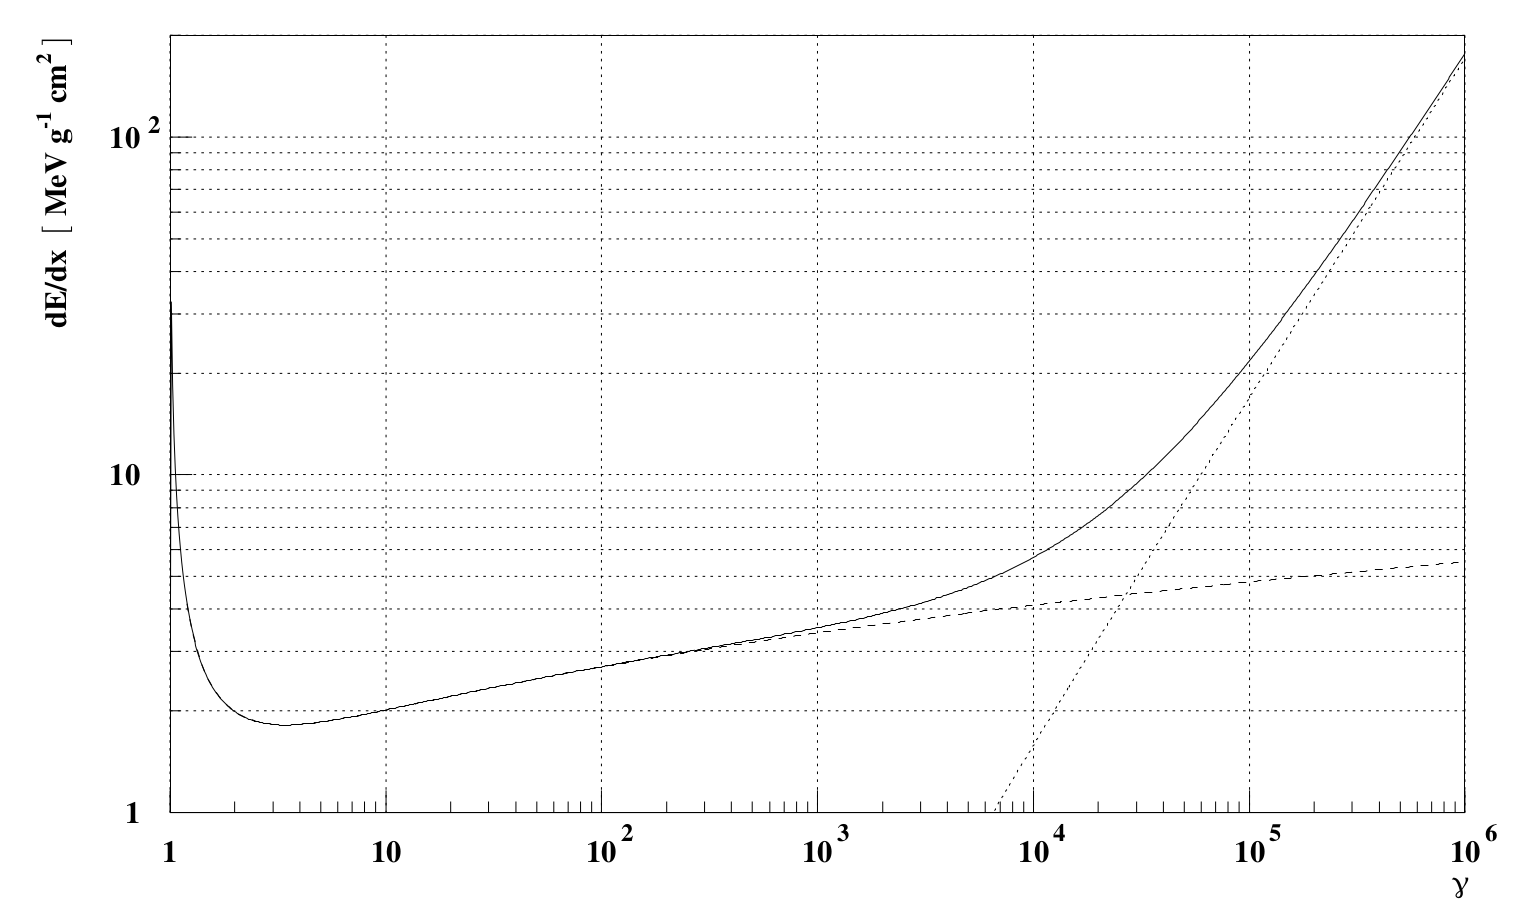
\includegraphics[width=0.7\textwidth]{Figs/Bethe_Muons.png}
        \caption[Ecuación de Bethe-Bloch para los muones.]{Pérdida de energía de Muones en el aire como función del factor de Lorentz \cite{Heck1998}. Están indicadas las contribuciones de la ionización (línea seccionada) y la producción de pares (línea punteada).}
        \label{fig:fig4}
\end{figure}

La \textbf{Dispersión múltiple de Coulomb} que ocurre cuando las partículas cargadas son dispersadas por el campo eléctrico Coulombiano de los núcleos de aire. Allí la dirección de propagación es alterada pero no cambia la energía de la partícula. La distribución angular de esta dispersión es descrita por la teoría de Moliére (\cite{Heck1998}).  

\subsection{Interacciones hadrónicas}
%%%%% NEW
Las interacciones hadrónicas son un componente fundamental en el estudio de las lluvias atmosféricas extensas (EAS). Aunque la cromodinámica cuántica (QCD) proporciona una base sólida para entender las interacciones fuertes, los procesos con múltiples partículas producidas en las interacciones hadrónicas aún no pueden ser calculados con precisión. Para superar esta limitación, se han desarrollado modelos que hacen suposiciones adicionales y utilizan parametrizaciones fenomenológicas y empíricas (\cite{Allen}).

Estos modelos son esenciales para interpretar las EAS y deben estar optimizados para un amplio rango de energías. Además, es crucial que se actualicen constantemente a medida que se obtienen más datos de los aceleradores o de grandes instrumentos como el Observatorio Pierre Auger \cite{andrada_2021}. Las interacciones hadrónicas generan piones cargados y neutros ($\pi^{-},\pi^{+},\pi^{0}$), así como kaones, que tienen una tendencia mayor a decaer que a interactuar. Los canales de decaimiento más probables para estas partículas son los siguientes:
\begin{equation*}
\pi^{0} \rightarrow \gamma\gamma \quad [{98.823 \pm 0.034}{\%}] \quad y
\end{equation*}

\begin{equation}
\pi^{0} \rightarrow e^{+}e^{-} \gamma \quad [{1.174 \pm 0.035}{\%}] .
\end{equation}

\begin{equation*}
\pi^{+} \rightarrow \mu^{+}\nu_{\mu} \quad [{99.98 \pm 0.00004}{\%}] \quad y
\end{equation*}
%
\begin{equation}
\pi^{-} \rightarrow \mu^{-}\nu_{\mu} \quad [{99.98 \pm 0.00004}{\%}] .
\end{equation}

\begin{equation*}
K^{+} \rightarrow \mu^{+}\nu_{\mu} \quad [{63.56 \pm 0.11}{\%}],
\end{equation*}
%
\begin{equation}
K^{+} \rightarrow \pi^{0}e^{+}\nu_{e} \quad [{5.07 \pm 0.004}{\%}],
\end{equation}
%
\begin{equation*}
K^{+} \rightarrow \pi^{+}\pi^{0} \quad [{20.67 \pm 0.08}{\%}] \quad y
\end{equation*}
%
\begin{equation*}
K^{+} \rightarrow \pi^{+}\pi^{+}\pi^{-} \quad [{5.583 \pm 0.024}{\%}] .
\end{equation*}
Que contribuyen a la componente electromagnética y muónica de las EAS. Más específicamente, componente muónica en las EAS es de particular interés debido a las propiedades relativistas de los muones y su larga vida media. Esta componente ofrece una visión directa de las primeras interacciones hadrónicas y las propiedades del hadrón inicial. Los muones de alta energía desencadenan sub-cascadas electromagnéticas y hadrónicas en la lluvia a través de interacciones tipo:
\begin{equation}
\mu^{\pm} \quad \xrightarrow{Y^{A}_{Z}} \quad \mu^{\pm}e^{+}e^{-},
\end{equation}
\begin{equation}
\mu^{\pm} \quad \xrightarrow{Y^{A}_{Z}} \quad \mu^{\pm} + hadrones.
\end{equation}  
%%%%%%%%%%%%%%%%%%%%%%%%%%%%%%%%%%%%%%%%%%%%%%%%%%%%%%%%%
%%%%%%%%%%%%%%%%%%%%%%%%%%%%----->SECCIÓN 3<-----%%%%%%%%%%%%%%%%%%%%%%%%%
\newpage
\newpage

\chapter{El Observatorio Pierre Auger}

El Observatorio Pierre Auger es el observatorio de CR más grande del mundo, con un área de detección de alrededor de $3000 km^{2}$. Su objetivo principal es detectar CR de ultra alta energía $(E > 10^{18} eV)$, cuya tasa de arribo a la tierra está entre 1 partícula $km^{2}/year$ a 1 partícula $km^{2}/century$. El observatorio es un arreglo híbrido, que está constituido principalmente por dos tipos de detectores: los telescopios de fluorescencia atmosférica y los detectores Cherenkov de superficie. Este detector híbrido proporciona estadísticas de alto nivel y reduce las incertidumbres sistemáticas en la medición de las energías de los CR \cite{allekotte_2008}. En este capítulo, revisaremos las generalidades de cada uno de estos detectores, enfocándonos en los detectores de superficie y sus mecanismos para la identificación de partículas.

\section{Detector de Fluorescencia}
El detector de fluorescencia está diseñado para registrar el desarrollo longitudinal de las lluvias de partículas secundarias generadas por CR de muy alta energía. Esto es posible gracias a que al propagarse por la atmósfera los CR secundarios excitan el nitrógeno liberando luz fluorescente en el rango de 300 nm a 430 nm. El criterio principal de su diseño es la detección de cada lluvia con energías de al menos $10^{19}eV$ (\cite{FD_auger}). Este arreglo consta de 24 telescopios independientes distribuidos en 4 sitios, cada uno con un campo de visión de $30^{\circ} \times 30^{\circ}$  como se observa en la figura \ref{fd_auger}. En este instrumento, el número de fotones producidos es proporcional a la energía de la componente electromagnética de la lluvia y al número total de partículas generadas a cierta profundidad atmosférica (\cite{FD_auger}).

\begin{figure}[!ht]
\centering
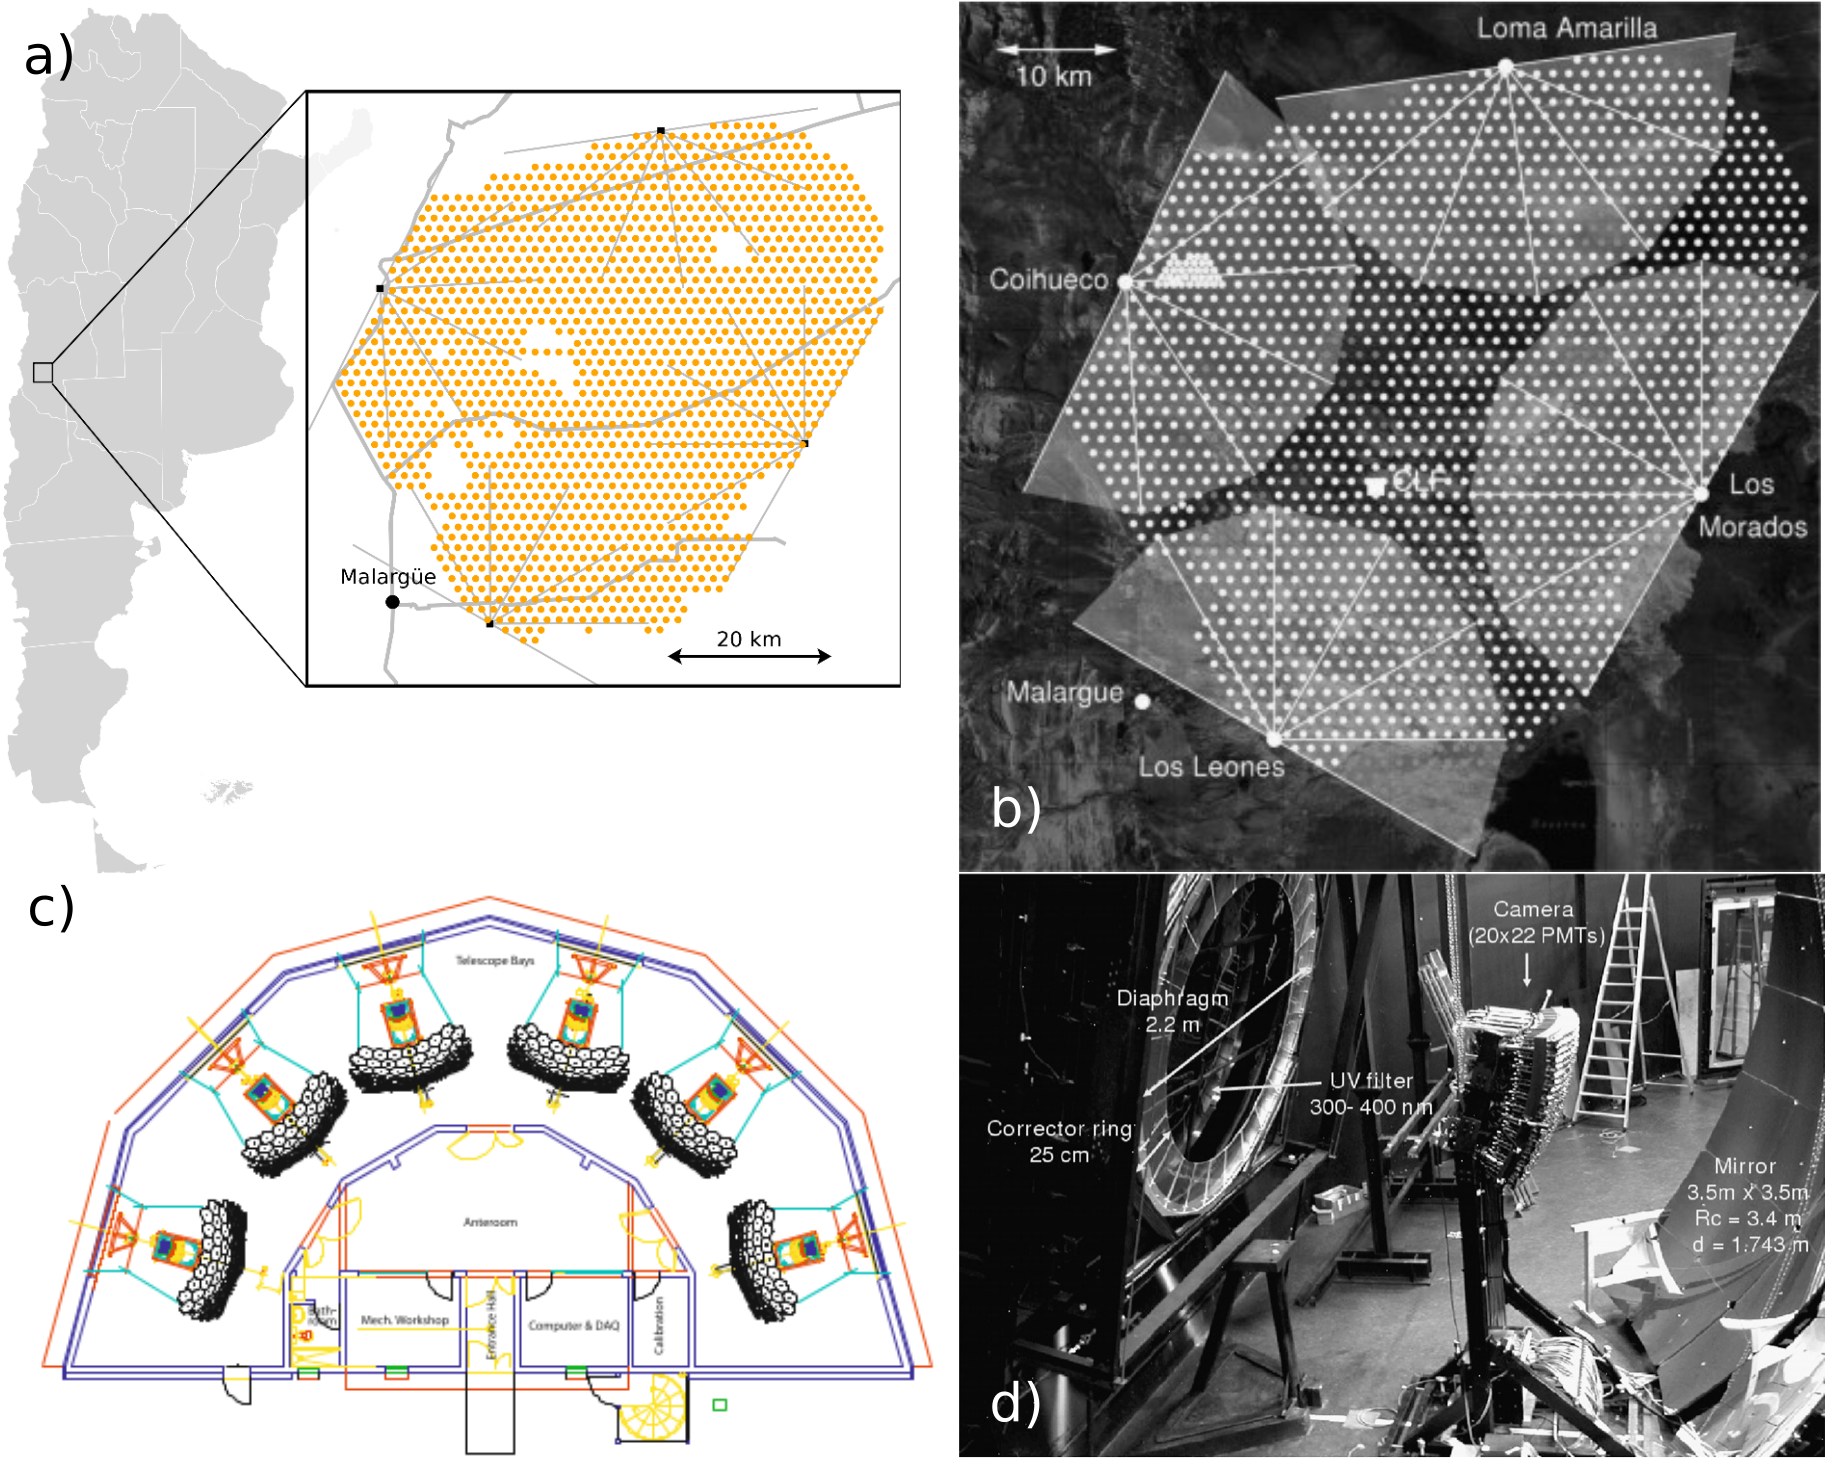
\includegraphics[width=1\textwidth]{Figs/FD_auger_composition.png}
\caption{a) Mapa donde se muestra la ubicación del Observatorio Pierre Auger y sus sistemas detectores. Los puntos amarillos corresponden a los detectores de superficie, y los 4 puntos negros en las fronteras, corresponden a la ubicación de los detectores de fluorescencia (\cite{asorey_2012}). b) Los puntos grises muestran las posiciones de las estaciones de detectores de superficie. Los semicírculos en gris claro indican los campos de visión de 24 telescopios de fluorescencia situados en cuatro edificios en el perímetro de los detectores de superficie (\cite{FD_auger}). c) Esquema de uno de los cuatro edificios con seis telescopios de fluorescencia en su interior logrando un campo de visión de $180^{o}$ (\cite{FD_auger}). d) Estructura de un telescopio de fluorescencia. El sistema de apertura consta de un diafragma, un anillo corrector y un filtro UV. Los componentes ópticos que corresponden al espejo, la cámara y un conjunto de 20x22 PMT (\cite{dedonato_2007}).}
\label{fd_auger}
\end{figure}

El arreglo utiliza un filtro UV para dejar pasar solo luz ultravioleta en el rango de 330 nm a 380 nm que corresponde al rango de interés para las observaciones. Además, los telescopios están diseñados para funcionar únicamente durante noches despejadas sin Luna, lo que reduce el ruido de fondo y mejora la precisión de las mediciones. 

\section{Detector de superficie}

El Observatorio cuenta con un detector de superficie que comprende una matriz de 1660 estaciones de detectores Cherenkov de agua (WCD) abarcando un área total de $3000$ $km^{2}$. Estas estaciones están distribuidas en una red hexagonal de $1.5$ $km$ de espaciado (ver figura \ref{fd_auger}). Dicha configuración está diseñada para estudiar el desarrollo transversal de todas las lluvias de partículas generadas por primarios de al menos $10^{18}$ $eV$ a nivel del suelo.

Dado el tamaño del área cubierta, las estaciones deben operar de manera autónoma y requerir poco mantenimiento (\cite{allekotte_2008}). Por lo tanto, estos detectores están interconectados a través de una red inalámbrica de área local, cuyo receptor principal es el telescopio de fluorescencia más cercano, que se encarga de transmitir los datos a la central de recopilación principal CDAS.

\subsection{Efecto Cherenkov}

Cuando una partícula con carga se mueve a través de un medio, su pérdida de energía aumentará a medida que la densidad del medio se incremente. Si consideramos que la densidad $\rho$ del medio es constante y que \textit{b} es el parámetro de impacto, la energía que pierde la partícula al atravesar una sección de longitud \textit{dl} dentro de un cilindro de radio \textit{a}, cuyo eje coincide con la dirección de movimiento, se puede expresar como $\frac{dE}{dl} = \rho \frac{dE}{dX}$. Esta pérdida de energía está determinada por el flujo del vector de Poynting, con la componente longitudinal $E_{1}$ del campo eléctrico, y con la componente transversal del campo magnético $B_{3}$ presentes en el medio, en función de la frecuencia $\omega$ (\cite{fermi_1940}).
\begin{equation}
    \frac{dE}{dl} = -ca \mathcal{R}\left(\int_{0}^{\infty} B^{*}E_{1}(\omega) \, d\omega\right)
    \label{fermi1}
\end{equation}
%%%%%%%%%%%%%%%%% PARENTESISSSSS
Consideremos una partícula cargada que se desplaza a una velocidad $v=\beta c$ a través de un medio con una constante dieléctrica $\epsilon(\omega)$ y un número atómico $Z$. En este escenario, la longitud de onda de la radiación emitida se modificará debido a la presencia del medio de la siguiente manera:
\begin{equation}
\lambda^{2}=\frac{\omega^{2}}{v^{2}}(1-\beta^{2}\epsilon(\omega)).
\label{lamdamod}
\end{equation}
Teniendo en cuenta las expresiones para los campos $E$ y $B$, el integrando de la ecuación \ref{fermi1} obtenemos:
\begin{equation}
B^{*}_{3}(\omega)E_{1}(\omega)=\left(\frac{Ze}{c}\right)^2 \left(-i\sqrt{\frac{\lambda^{*}}{\lambda}}\right)\left(1-\frac{1}{\beta^{2}\epsilon(\omega)}\right)exp[-a(\lambda+\lambda^{*})]\omega.
\end{equation}
En este caso, si $\lambda$ es un número imaginario puro, $\lambda^{*}=-\lambda$ lo que haría 
$exp[-a(\lambda+\lambda^{*})] = 1$ y por consiguiente la expresión \ref{fermi1} sería independiente de $a$, donde parte de la energía escapa al infinito en forma de emisión coherente de radiación (\cite{asorey_2012}). Esto sucede si $\epsilon$ es real, es decir que el medio no es absorbente y que $\beta^{2}\epsilon(\omega)>1$ ó $\beta=\frac{1}{\sqrt{\epsilon(\omega)}}$. En otras palabras, si la velocidad de la partícula cargada es mayor que la velocidad de la luz en el medio a una frecuencia $\omega$, fenómeno conocido como \textit{Efecto Cherenkov} (\cite{asorey_2012}).

Si el medio es ligeramente absorbente la expresión \ref{fermi1} queda como:
\begin{equation}
\left(\frac{dE}{dl}\right)_{Cherenkov}=\left(\frac{Ze}{c}\right)^{2}\int_{\beta^{2}\epsilon(\omega)>1} \omega\left(1-\frac{1}{\beta^{2}\epsilon(\omega)}\right)d\omega
\end{equation}
donde se observa que la emisión de radiación depende de la frecuencia. En el caso del agua, en el espectro visible, la radiación Cherenkov se produce a longitudes de onda cortas, donde  $n(\omega) \approx \sqrt{\epsilon(\omega)}$ aumenta levemente con la frecuencia. El ángulo de emisión de la radiación está definido entonces por:
\begin{equation}
cos\theta_{c}=\frac{1}{\beta\sqrt{\epsilon(\omega)}},
\end{equation}
Para el rango de frecuencias de interés (cerca del ultravioleta), el valor del índice de refracción puede ser considerado constante, con lo que podemos obtener el número de fotones Cherenkov producidos en un intervalo de longitudes de onda como sigue,
\begin{equation}
N=2\pi \alpha_{EM}l\left(1-\frac{1}{\beta^{2}n^{2}}\right)\left(\frac{1}{\lambda_{2}}-\frac{1}{\lambda_{1}}\right).
\label{cherenkovnumber}
\end{equation}


%%%%%%%%%%%%%%%%% PARENTESISSSSS

%EN ALGÚN MOMENTO DE LA VIDA \hbar cambió por \hslash en esta joda y no me enteré....

Donde $\alpha_{EM}=(e^2/ \hslash c)$ es la constante de estructura fina. Además, el momento de una partícula con masa en reposo $m_{0}$ y velocidad $\beta c$ es $p\equiv mv = \beta \gamma m_{0}c$, lo que permite calcular el número de fotones emitidos por una partícula con momento $p$ al recorrer una longitud $l$ en un medio con índice de refracción $n$. En el caso de los tubos fotomultiplicadores (PMT) utilizados en el Observatorio Pierre Auger, que son sensibles al rango de $300 - 570nm$, es posible definir dos propiedades clave en la respuesta posterior de los detectores Cherenkov:
\begin{itemize}
\item La radiación solo se emite cuando $\beta>1/n$.
\item El número de fotones emitidos por unidad de longitud tiende a un valor constante (ver figura \ref{stopping_cherenkov}), que solo depende del rango de longitudes de onda considerado, del índice de refracción del medio y la distancia recorrida en dicho medio. De esta manera, la señal en el detector no proviene de la energía depositada, sino de la cantidad de fotones producidos, es decir, de la distancia recorrida por la partícula en el agua (\cite{asorey_2012}).
\end{itemize}
\begin{figure}
\centering
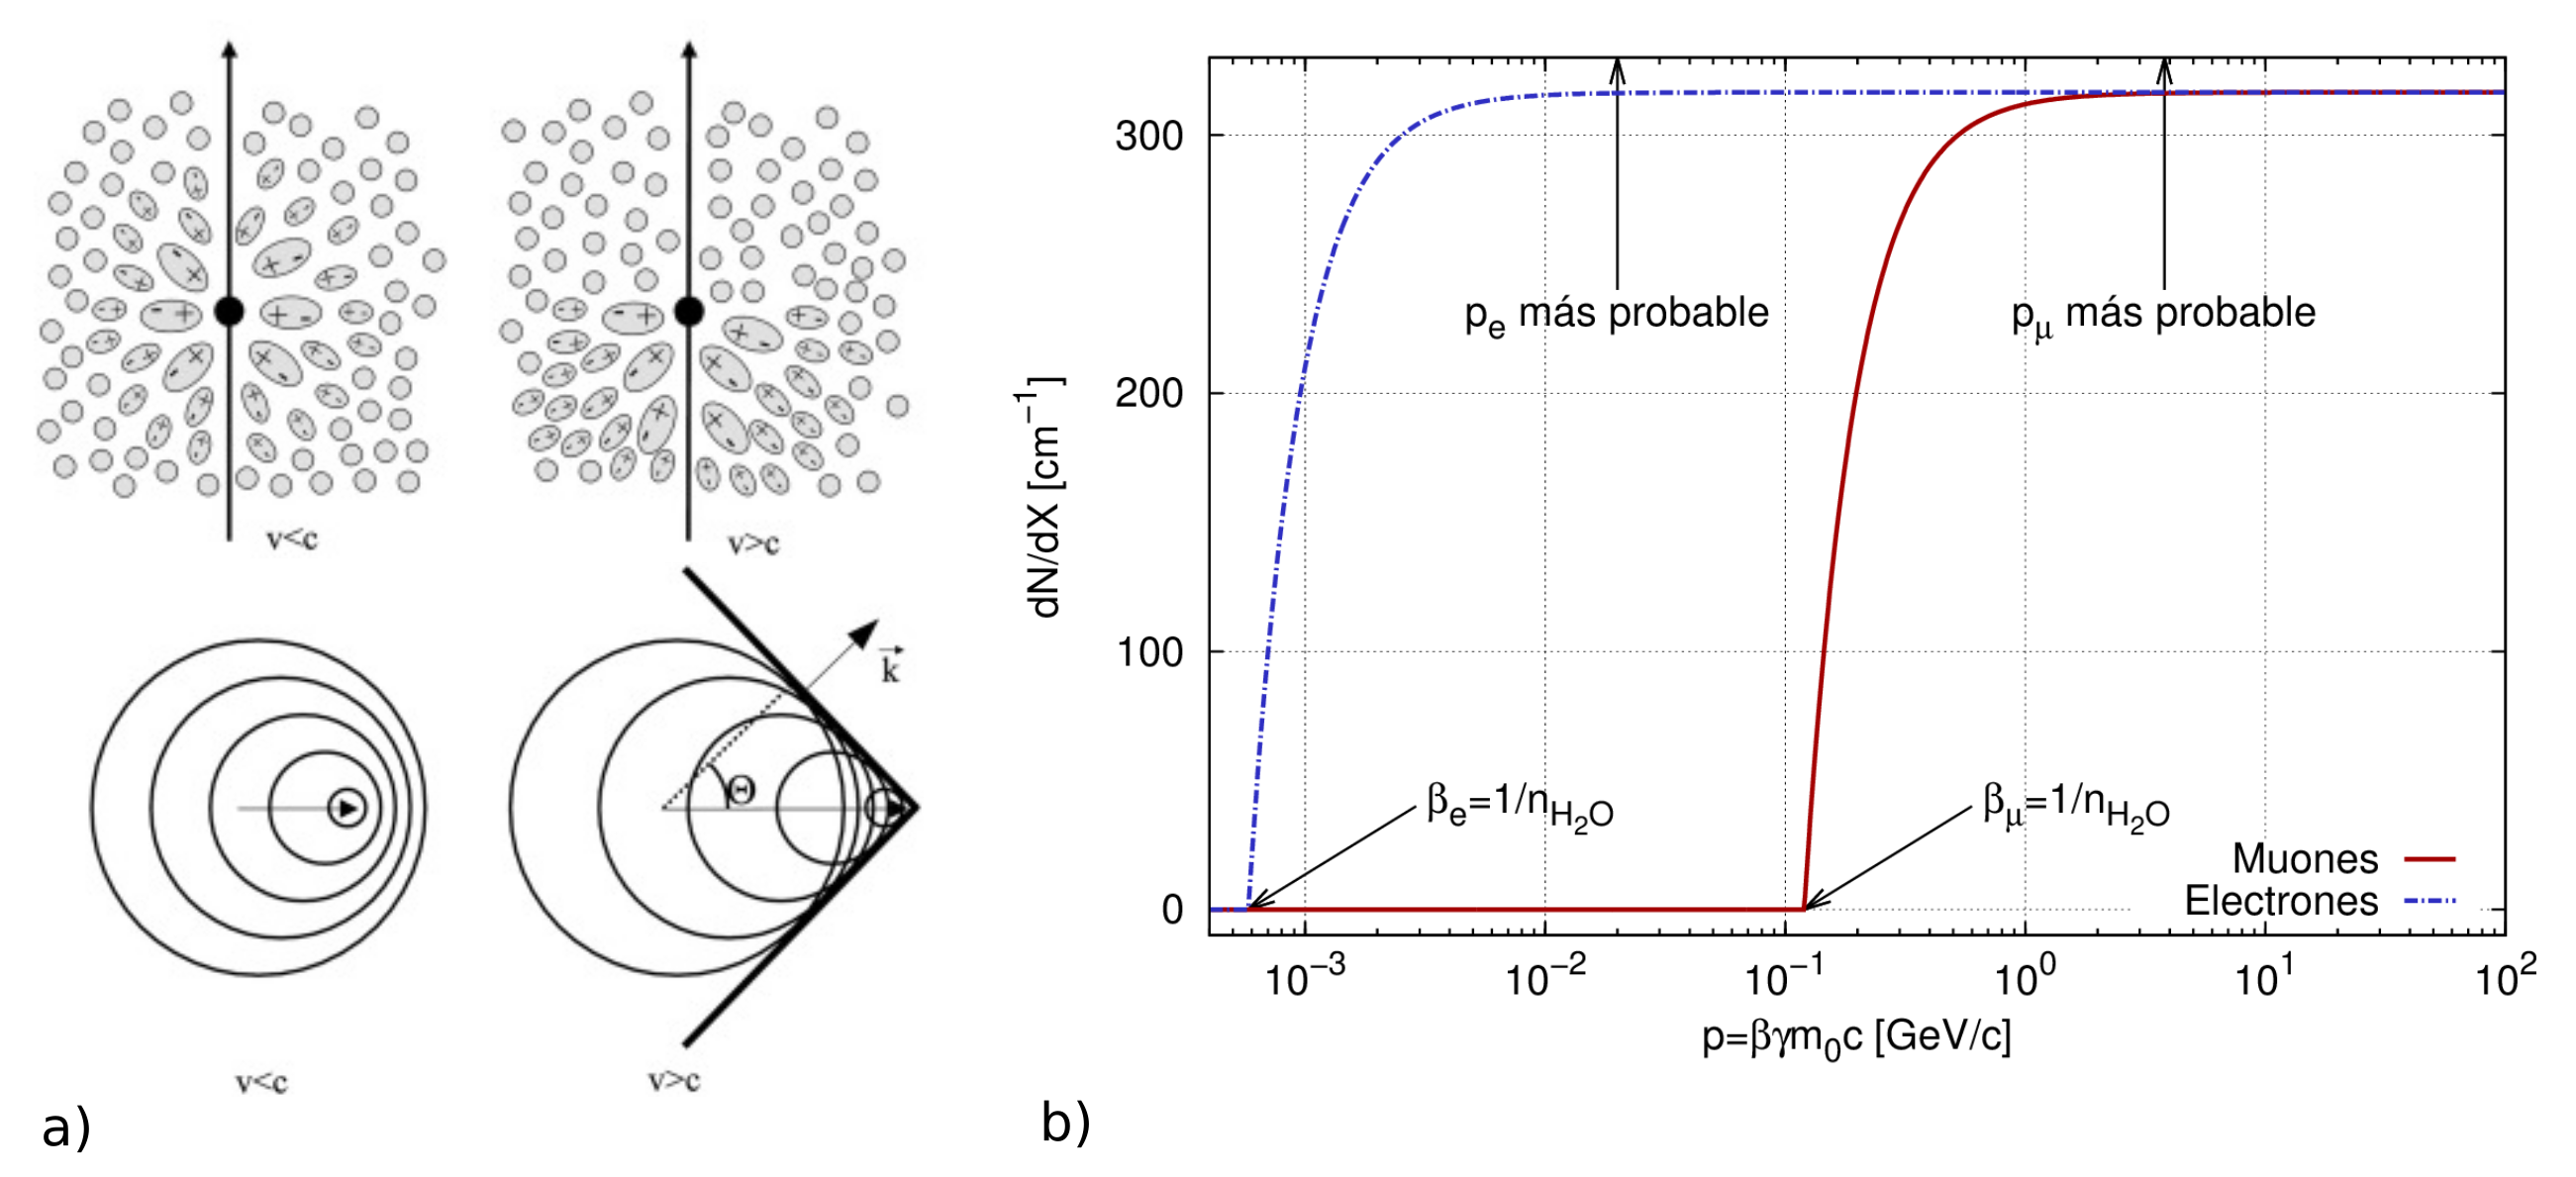
\includegraphics[width=1\textwidth]{Figs/cherenkov_stopping.png}
\caption{a) Arriba: ilustración de la polarización del medio inducida por el paso de una partícula relativista. Abajo: Construcción del frente de onda de Cherenkov. Fuente: \cite{deNaurois:2015oda} b) Esquema Producción de fotones Cherenkov en la banda $300 nm < \lambda < 570 nm$ según la ecuación \ref{cherenkovnumber} como función del impulso. La línea punteada corresponde a un electrón y la sólida a un muón luego de haber recorrido 1 cm en agua líquida. Se puede observar que la cantidad de fotones tiende rápidamente a un valor constante de $\thicksim 315$ fotones por centímetro incluyendo el momento más probable para las dos partículas. Fuente \cite{asorey_2012}}
\label{stopping_cherenkov}
\end{figure}
\subsection{El detector Cherenkov}
 
%Para ampliar las capacidades del observatorio a energías más bajas, también se despliega una región de relleno de estaciones SD con un espaciado de 750 m (SD-750) [68]. 
Cada detector de superficie se compone de un recipiente cilíndrico con una base de 10 $m^{2}$, lleno con 12 $m^{3}$ de agua de alta pureza que permite una mínima absorción de luz ultravioleta cercana. Esta agua se encuentra dentro de una bolsa fabricada con Tyvek, un material reflectante (ver figura \ref{fig:SD_auger}). Cuando las partículas relativistas atraviesan el volumen de agua, generan radiación Cherenkov que es reflejada y dispersada por el Tyvek en el interior del recipiente, lo que incrementa la probabilidad de detección (\cite{allekotte_2008}).

Esta radiación es captada por tres PMT Photonis XP1805/D1 de 9 pulgadas de diámetro (\cite{bertou_2006},\cite{allekotte_2008}), dispuestos de forma simétrica en la parte superior del tanque. Las señales analógicas de los PMT son convertidas a formato digital en la electrónica de la estación mediante convertidores de tipo flash de analógico a digital (FADC). Cada PMT registra el pulso que genera la detección de fotoelectrones que se caracteriza por tener un crecimiento rápido y un posterior decaimiento exponencial como se muestra en la figura \ref{fig:PMT} (\cite{asorey_2012}).

%Cada SD consta de un tanque cilíndrico de 10$m^{2}$ de base con 12 $m^{3}$ de agua ultra pura que permita una baja absorción del ultravioleta cercano, dentro de una bolsa con un material reflectante realizada en Tyvek. La radiación Cherenkov producida por el paso de partículas relativistas a través del volumen de agua, es reflejada y difundida por el Tyvek en el interior, maximizando la probabilidad de detección \cite{asorey_2012} y es registrada con tresPMT(PMT) Photonis XP1805/D1 de 9 pulgadas de diámetro, (\cite{Aab_2015}) colocados simétricamente en la parte superior del tanque. Las señales analógicas provenientes de los PMT son digitalizadas en la electrónica de las estación mediante conversores analógicos digitales tipo flash (FADC).
\begin{figure}[!ht]
  \centering
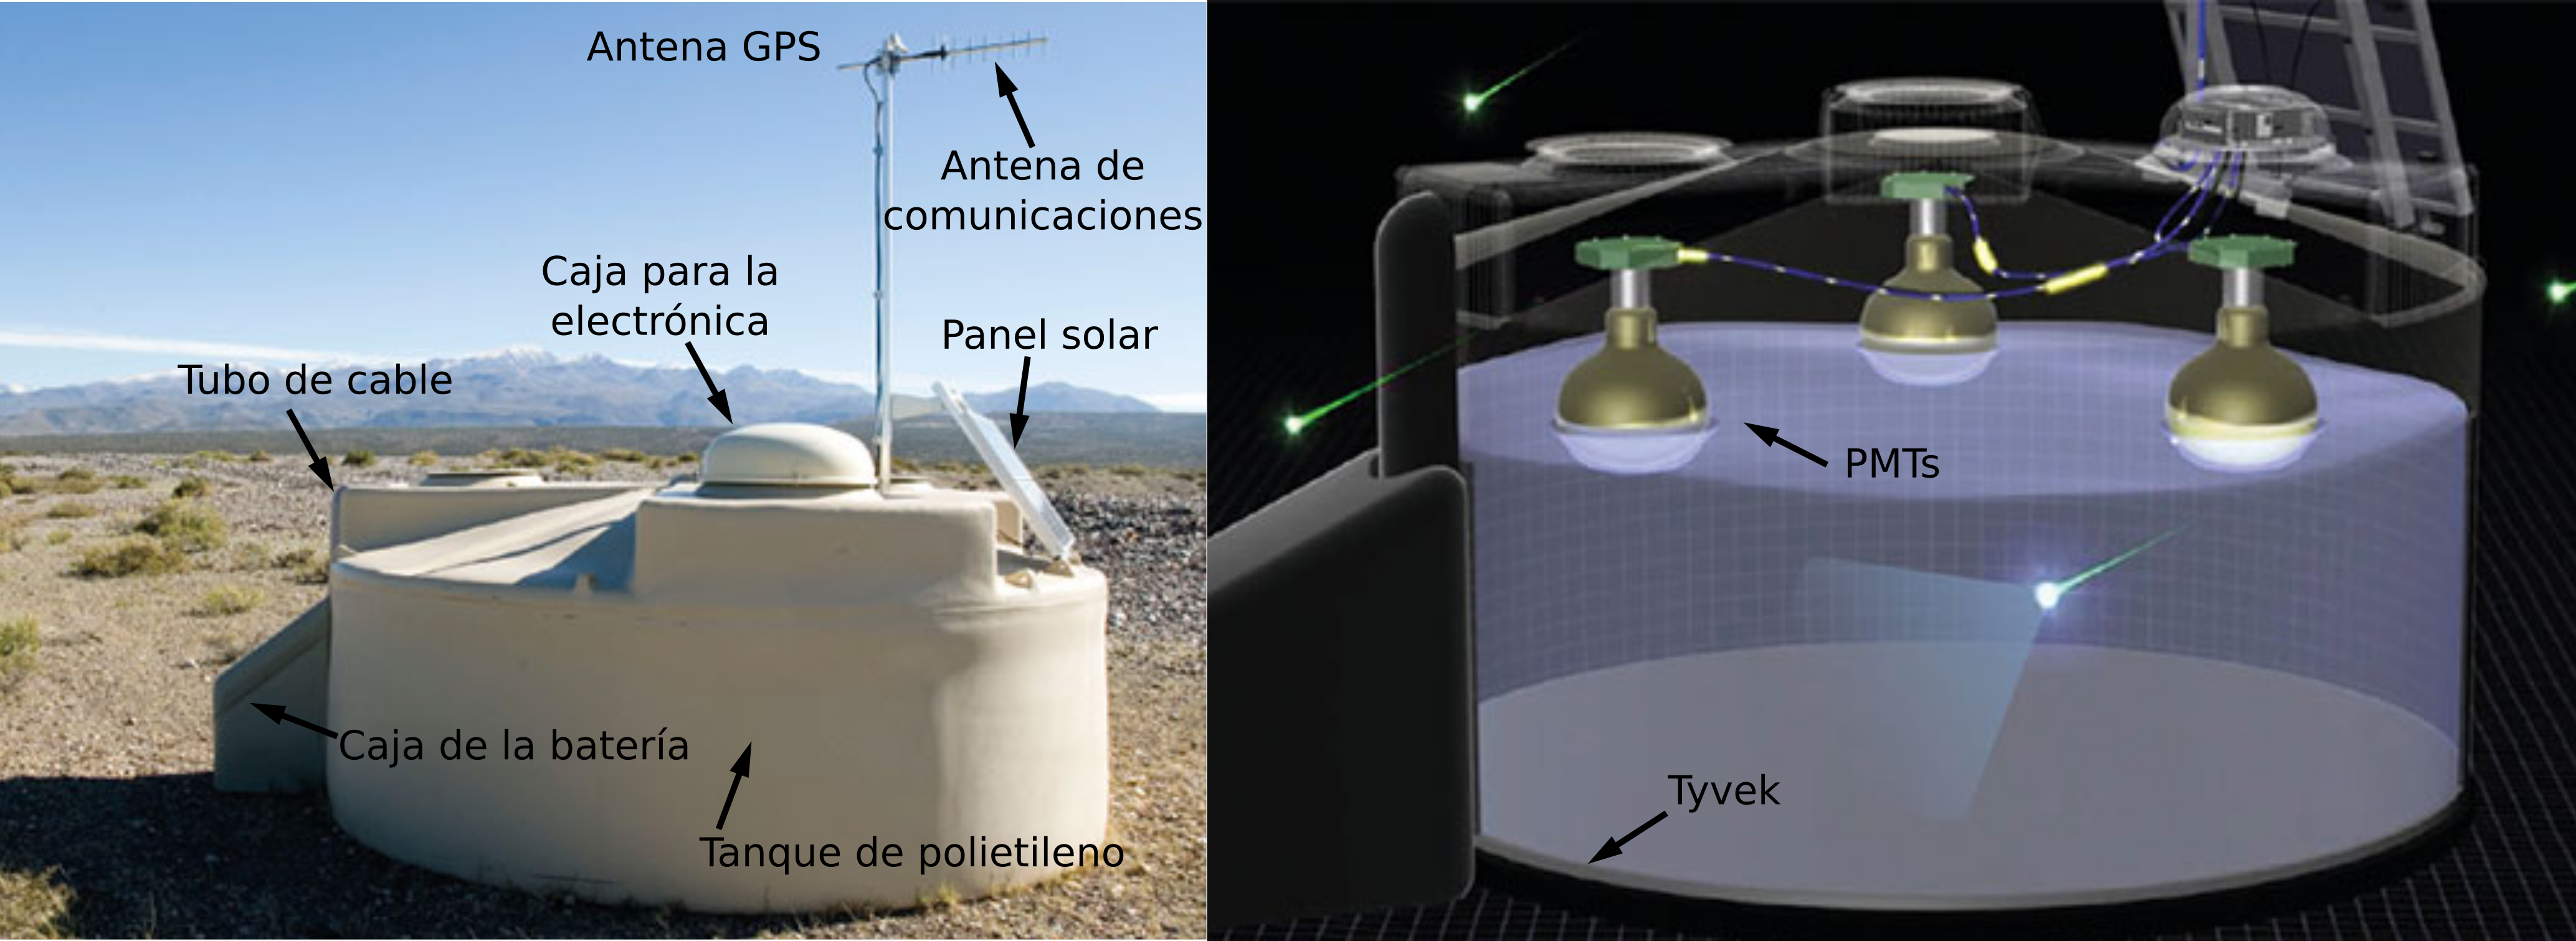
\includegraphics[width=0.8\textwidth]{Figs/SD_componentes.png}
  \caption{Estructura de un detector de superficie. A la izquierda se observa el exterior de un detector WCD del Observatorio ubicado en la Pampa Amarilla. A la derecha vemos una representación de su interior: Al entrar la partícula cargada al agua se produce un cono de luz Cherenkov, estos fotones son reflejados por las paredes del detector y recogidos por los PMT ubicados simétricamente en la superficie superior. \cite{allekotte_2008}}
  \label{fig:SD_auger}
\end{figure}



\begin{figure}[h!]
  \centering
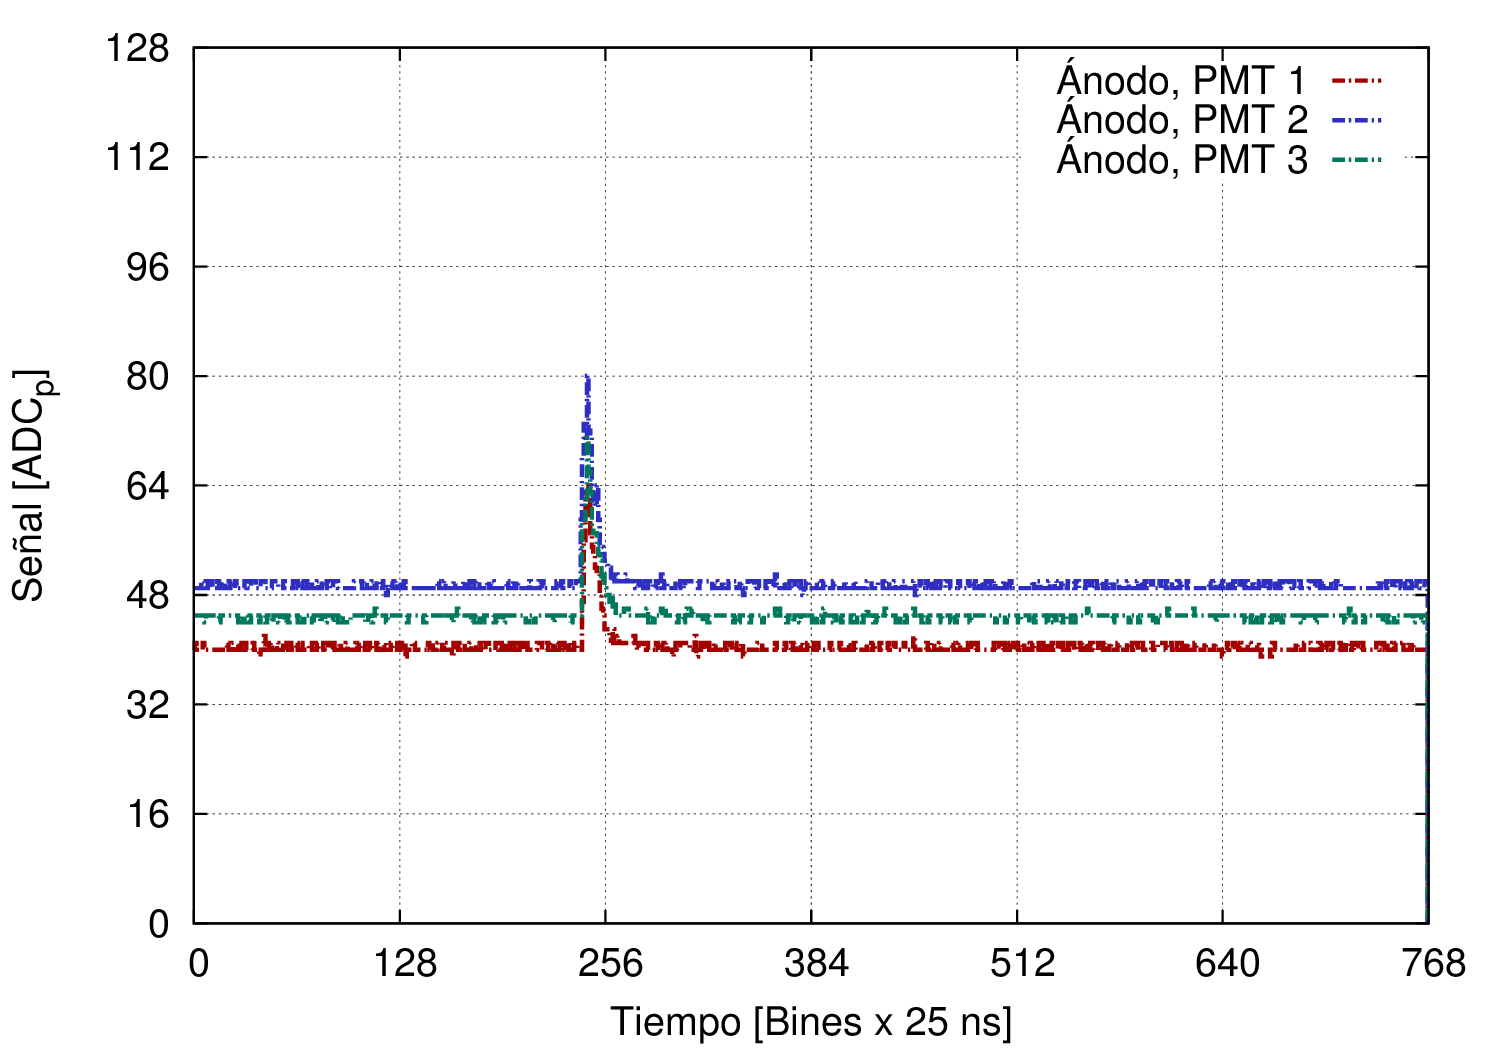
\includegraphics[width=0.6\textwidth]{Figs/PMTs_signal.png}
  \caption{Señal del ánodo de cada PMT. Estas señales son digitalizadas mediante seis conversores FADC de 10 bits a una velocidad de muestreo de 40 MHz. La traza consiste en un bloque contiguo de 768 bines de señal de 25 ns cada uno, totalizando $19.2 \mu s$. Fuente: (\cite{asorey_2012})}
  \label{fig:PMT}
\end{figure}
Una de las ventajas de usar detectores Cherenkov es que se puede diferenciar el paso de los muones (o su decaimiento) y la absorción de los electrones. Los muones atmosféricos (con energías típicas de $E_\mu \thicksim 3GeV$), depositan en el detector solo una pequeña fracción de su energía cinética de tal forma que son capaces de atravesarlo (\cite{asorey_2012}). La señal Cherenkov producida por muones depende únicamente de la longitud recorrida en el agua, determinada por la geometría del detector y la dirección del muón. Para muones con $E_\mu < 390 MeV$, su rango es menor que la profundidad del detector en posición vertical. Estos muones depositan toda su energía en el detector y pueden decaer en su interior.
%(El poder de frenado de muones en agua es de $\thicksim 2 MeV cm^{-1}$ en un amplio rango de energías) 
Por el contrario, los electrones cuyo rango de energía típico es de $\thicksim 20MeV$, poseen un poder de frenado de $\thicksim 2MeV cm^{-1}$, lo que provoca que al ingresar al agua se produzca una absorción total en el volumen del detector. El número total de fotones producidos, y por ende la señal registrada, muestra una fuerte dependencia de la energía inicial del electrón, alcanzando un máximo para trayectorias verticales que atraviesan completamente el detector ($\thicksim 3.8 x 10^{4}$ fotones). De esta forma, el detector actúa como calorímetro de electrones absorbiendo toda su energía cinética, la señal que se registra está relacionada solo con la emisión de fotones Cherenkov que se detiene antes de absorber completamente al electrón (\cite{masias_2017}). 

La diferenciación entre las señales producidas por fotones y muones se evidencia en la figura \ref{cargahist} donde contrasta la carga depositada durante un tiempo y medida por un tubo fotomultiplicador del observatorio. El pico inicial refleja la distribución de señales principalmente generadas por la componente electromagnética, sumada al efecto del umbral de detección. El segundo pico, por su parte, se relaciona con el paso de muones que atraviesan verticalmente el detector. La posición del pico para un muón central y vertical medido por un PMT del Observatorio es de $(1.03\pm0.02)$ (\cite{asorey_2012}).

\begin{figure}[h!]
  \centering
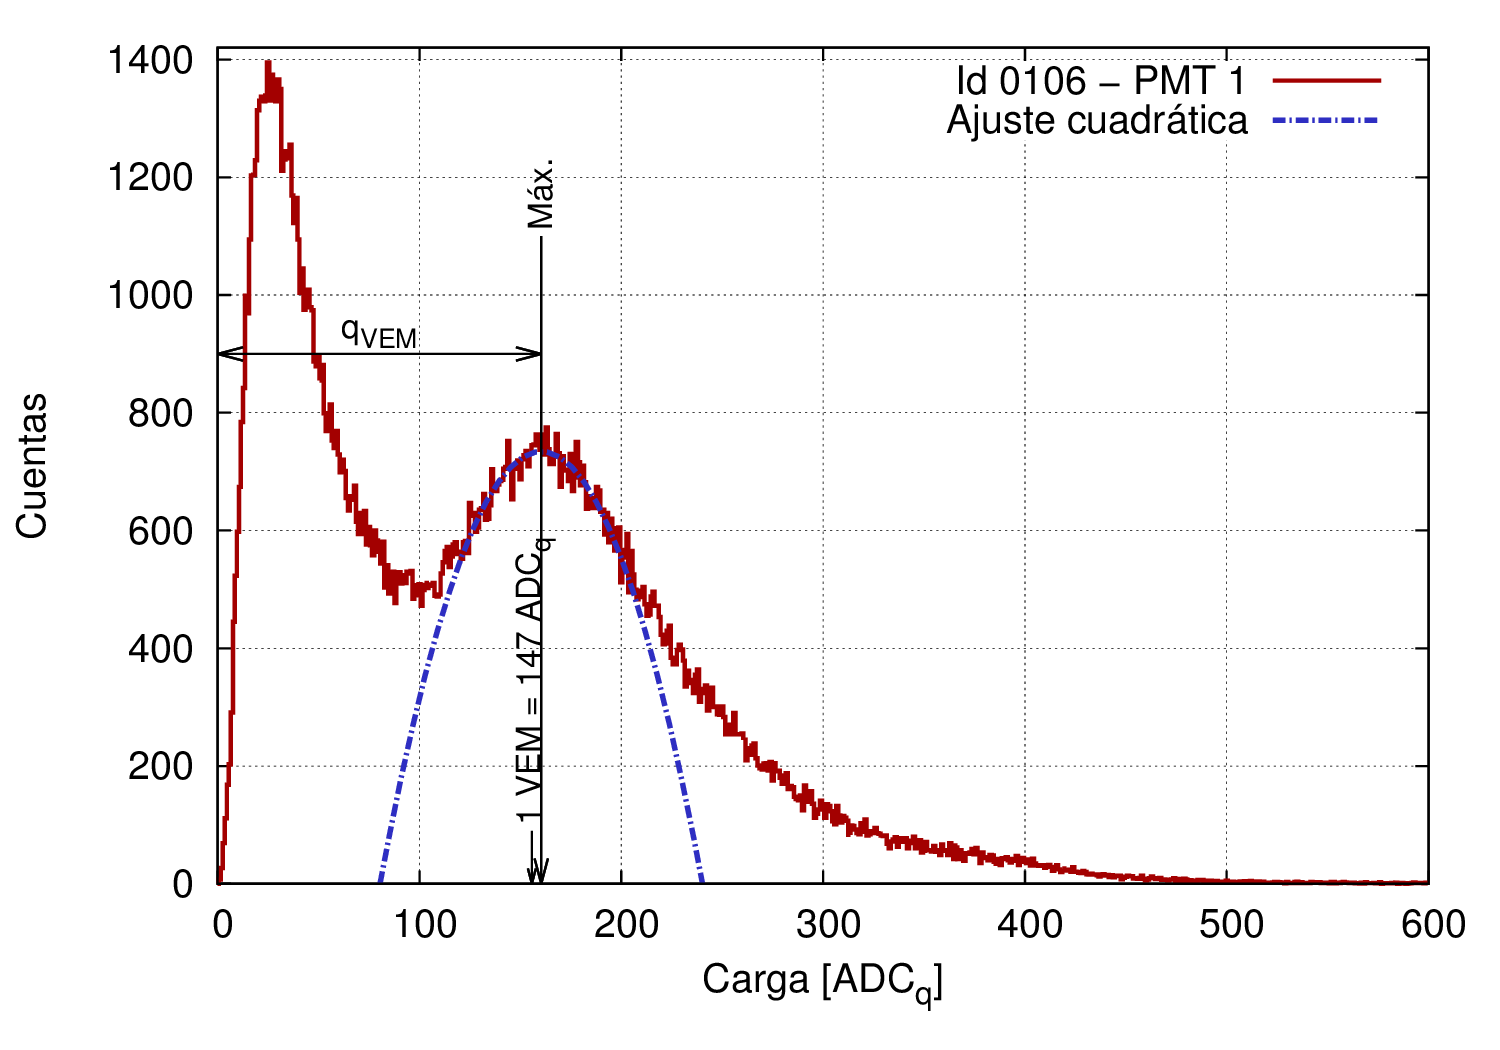
\includegraphics[width=0.6\textwidth]{Figs/histograma_carga.png}
  \caption{Carga depositada durante un tiempo y medida por un tubo fotomultiplicador del observatorio. El pico inicial refleja la distribución de señales principalmente generadas por la componente electromagnética, sumada al efecto del umbral de detección. El segundo pico, por su parte, se relaciona con el paso de muones que atraviesan verticalmente el detector. Fuente: (\cite{asorey_2012})}
  \label{cargahist}
\end{figure}
Algunos parámetros de importancia referentes a los detectores Cherenkov del Observatorio que serán necesarios para las secciones siguientes son:
\begin{itemize}
\item     \textbf{Bin de la señal:} Intervalo entre dos pulsos sucesivos. Considerando que el conversor tiene una tasa de muestreo de 40MHz, se establece que $1bin\equiv \frac{1}{40MHz} = 25ns$
    \item \textbf{Cuentas ADC de pico:} Es la magnitud correspondiente al valor de salida del conversor FADC de tal forma que $1ADC_{p}= 1.95mV$ 
    \item \textbf{Cuenas ADC de carga:} Unidad luego de integrar temporalmente la señal en $ADC_{p}$, restando la línea base.
    \item \textbf{$VEM$ (\textit{Vertical Equivalent Muon}):} Es la carga total depositada por un muón que atraviesa completamente a un detector de superficie de forma vertical, un $VCM$ (\textit{muón central y vertical}). $1VEM=\frac{q_{VEM}}{1.03}ADC_{q}=240MeV$.
    \item \textbf{$VEM_{p}$:} Es el equivalente a la altura máxima del pulso típico de la señal producido por un $MCV$: $1VEM_{P}=\frac{I_{VEM}}{1.03}ADC_{p}=240MeV$.
    \item \textbf{Relación carga sobre pico $AoP$: } Es la relación de las cargas integradas $(ADC_{q})$ y los voltajes $(ADC_{p})$ en la zona de pico de muones del histograma de tal forma que: $AoP=\frac{ADC_{q}}{ADC_{p}}$ que correspondería a un parámetro fundamental de calibración. Con este parámetro posible tener una idea de la respuesta impulsional del detector frente a los muones, relacionando con cargas integradas.
    \item \textbf{Sistema de umbral (trigger):} Es la estructura de 5 niveles que se establecen sobre el nivel de detección para seleccionar las señales producidas por los CR de interés sobre el fondo, con el objetivo de descartar ruidos y eventos físicos no relevantes para el observatorio. A partir del sistema de Trigger se logra registrar de forma diaria un promedio de 3 eventos por detector (\cite{asorey_2012}).
\end{itemize}

\section{Medición del fondo de CR}

El fondo de CR secundarios en la superficie de la Tierra es el resultado de las interacciones de los CR galácticos (GCRs) y el viento solar con la atmósfera terrestre. Podría decirse que este fondo corresponde a un flujo constante de partículas que varía levemente debido a la actividad solar periódica y transitoria (\cite{masias_2017}). El Observatorio Pierre Auger, aunque está optimizado para la identificación de partículas de ultra alta energía, tiene dos modos de detección alternativos de baja energía que registran el flujo de partículas secundarias al nivel de los detectores de superficie: El modo scaler y el modo Histograma. En  este trabajo de investigación exploramos las características y propiedades del modo scaler aplicado al estudio del fondo de radiación natural y su variabilidad estrechamente relacionada con la actividad solar, aprovechando la capacidad de recolección de datos, la cantidad de detectores y la superficie cubierta por este arreglo.

\subsection{Modo scaler}

En 1997, se propuso la implementación en el observatorio de un modo de detección que estuviera destinado a caracterizar el fondo y  con este, identificar lluvias atmosféricas extendidas originadas por los fotones provenientes de GRBs (destellos de rayos gamma)(\cite{asorey_2012} , \cite{bertou_2011}). Los GRB consisten en una emisión súbita de rayos gamma en periodos cortos de tiempo ($\cdot 10^{-3}s - \cdot 10^{2}s$) que continúa en la emisión de fotones cada vez menos energéticos (rayos X hasta radio). El espectro en energía de los fotones gamma observados durante la ocurrencia de un GRB, muestran que podrían llegar hasta energías de varios GeV (\cite{Bernlöhr_1996}).
%El espectro de energía de los fotones gamma que han sido observados y reportados pueden llegar a energías en el rango de unidades de $GeV$ 

De esta forma se crea el modo scaler que consiste en determinar las tasas de conteo de pulsos individuales de cada detector de superficie en escalas de tiempo de un segundo \cite{asorey_2012}. Con este método, se puede determinar el flujo de fondo sobre el arreglo y a partir de éste, identificar excesos generados por fenómenos transitorios diversos como los GRB y también pueden dar una idea de la tasa de CR de baja energía influenciados por la modulación solar.

Como es de esperarse, no todas las señales registradas en el detector corresponden a datos válidos para la determinación de este flujo. En primer lugar, la diferencia entre la línea base y el voltaje del pico del pulso debe cumplir las siguientes condiciones:

\begin{itemize}
    \item Del 20 de Marzo hasta el 20 de Septiembre de 2005, este voltaje debe ser mayor a 3ADC
    \item Desde el 21 de Septiembre del 2005, la diferencia de voltajes debe comprender entre: $3ADC < (V_{p}-V_{b}) \leq 20ADC $
\end{itemize}

Esta diferencia de periodos se sustenta en la necesidad de implementar un umbral de detección superior que permita una mejor relación señal a ruido \cite{bertou_2007}, y así superar las limitaciones en los datos que se venían recolectando. Dichos cambios en los umbrales fueron implementados desde el 21 de Septiembre del 2005.

Los pulsos recopilados son guardados enviados una vez por segundo para su almacenamiento. Cada segundo de datos contiene: el tiempo en que se realizó el registro, número de estaciones activas, el número total de pulsos contados en todo el arreglo, y los conteos de pulsos para cada detector. Finalmente se obtiene un archivo de datos por día. Luego de esto, se deben eliminar los detectores que muestren inestabilidades respecto a la media, ruido producido por rayos, inestabilidades térmicas y relámpagos originados en tormentas eléctricas.  

\subsection{Modo histograma}

El modo Histograma permite estudiar la variación de la tasa de conteo en diferentes rangos de energía depositada, asociados con diversas energías primarias de GCR. En el sistema de detección del Observatorio, corresponde al registro de los pulsos del fondo de radiación en intervalos de tiempo de 61 segundos \cite{asorey_2012} . Estos registros permiten realizar la calibración del detector en un intervalo de tiempo determinado respecto a su respuesta impulsional y acompañan los eventos filtrados y almanecados por el sistema de trigger principal. 

Después del proceso de calibración, a partir del VEM se pueden construir histogramas de energía depositada de hasta aproximadamente 1 GeV. El modo Histograma permite estudiar la variación de la tasa de conteo en diferentes rangos de energía depositada, asociados con diversas energías primarias de CR galácticos (GCRs) (\cite{asorey_2012}, \cite{masias_2017}). Los dos rangos de energía de mayor interés son: el rango asociado a las energías depositadas en el modo scaler (energía entre 60 MeV y 120 MeV), y el relacionado con las energías depositadas por muones con incidencia vertical (energía entre 200 MeV y 280 MeV), también denominado \textit{banda muónica}. 

Los modos scaler e histograma están fuertemente relacionados puesto que la integral del histograma de carga, por construcción, representa el número de señales registradas en ese minuto. Ajustando adecuadamente los límites de esta integración, teóricamente debería ser posible recuperar las tasas de los scalers de ese detector (\cite{Martin_Schimassek2022}). 

%%%%%%%%%%%%%%%%%%%%%%%%%%%%----->SECCIÓN 3<-----%%%%%%%%%%%%%%%%%%%%%%%%%
\newpage
\chapter{Modulación del fondo de Rayos Cósmicos debido a la actividad Solar}

%%%%%%%%%%%%%%%%%%%%%%%%%%%%% NEWW
En este capítulo, presentaremos los resultados obtenidos del estudio de la modulación de los Rayos Cósmicos Galácticos (GCR) debido a la actividad solar, utilizando el Observatorio Pierre Auger. Aquí, nos encofaremos en examinar la sensibilidad del Observatorio Pierre Auger a las fluctuaciones en la actividad solar a corto y largo plazo.

Como se describió en el capítulo 1, la interacción entre los GCR y el viento solar provoca cambios en la cantidad de GCR detectados. El viento solar, que se ve afectado por fenómenos periódicos como la rotación solar de \~27 días, el ciclo de 11 años que está asociado a emisiones de plasma desde la corona y a un cambio en la frecuencia de las eyecciones de masa coronal (CME) (\cite{belov_2021} entre otros).

Los estudios previos realizados en el Observatorio han demostrado que el modo Scaler es altamente sensible a las condiciones del medio interplanetario determinadas por la actividad solar (\cite{Martin_Schimassek2022}). Esta sensibilidad permite que los datos recopilados en el modo Scaler proporcionen información complementaria a la obtenida a través de los monitores de neutrones, abriendo una ventana energética diferente a los rayos cósmicos de baja energía.

Comenzaremos con una descripción de los datos y las fuentes que hemos utilizado para este estudio, seguido de una explicación de cómo se procesaron los datos en modo Scaler del arreglo de detectores para garantizar la fiabilidad. A continuación, realizaremos una comparación entre las mediciones realizadas por Detectores de Neutrones y las obtenidas en el Observatorio Pierre Auger, destacando las ventajas y desventajas de cada uno en el contexto de nuestro estudio. Finalmente, discutiremos los efectos de la actividad solar en el fondo de rayos cósmicos a corto y largo plazo, proporcionando una visión completa de cómo la actividad solar puede influir en la detección de GCR.

\section{Datos}

En este trabajo, se utilizaron las siguientes bases de datos :
\begin{enumerate}

\item Scalers del Observatorio Pierre Auger: Se utilizaron datos de intensidad de rayos cósmicos del Observatorio Pierre Auger, corregidos por presión y temperatura utilizando el software \textit{ScalerAnalysis}\footnote{\url{https://opendata.auger.org/}}.
    \item Datos de detectores de neutrones: Se utilizaron datos de intensidad de rayos cósmicos de varias estaciones, incluyendo Oulu\footnote{\href{https://cosmicrays.oulu.fi/}{Cosmic Ray Station}  of the University of Oulu / Sodankyla Geophysical Observatory 
}, Athenas, México, y Tsumeb. Estos datos, con una resolución de 3 horas, fueron corregidos por presión y temperatura \footnote{Agradecemos el suministro de datos a la base de datos NMDB (www.nmdb.eu), creada en el marco del programa FP7 de la Unión Europea (contrato nº 213007).  \url{//www.nmdb.eu/nest/}}.
    \item Datos del viento solar: Se obtuvieron datos del viento solar del Space Physics Data Facility (SPDF) de la NASA \footnote{\url{https://spdf.gsfc.nasa.gov/pub/000_readme.htm}}.
    \item Datos de manchas solares: Se utilizaron datos de manchas solares del Centro de Datos Mundial SILSO, Real Observatorio de Bélgica, Bruselas (Sunspot Index and Long-term Solar Observations)(\cite{sidc})\footnote{\url{https://www.sidc.be/SILSO/datafiles}} . Es una parte del SIDC (Solar Influences Data Analysis Center), que es el departamento de física solar del Real Observatorio de Bélgica. SILSO se dedica a la producción, preservación y difusión del número internacional de manchas solares.
    \item Base de datos de Forbush Decreases: Se usó el Catálogo de los efectos Forbush y de las perturbaciones interplanetarias, creada por el Instituto Pushkov de Magnetismo Terrestre, Ionosfera y Propagación de Ondas de Radio de la Academia de Ciencias de Rusia (IZMIRAN). Esta base de datos es la única disponible que es integral y actualizada sobre los efectos de Forbush (\cite{okike_2021})\footnote{Instituto Pushkov de Magnetismo Terrestre, Ionosfera y Propagación de Ondas de Radio de la Academia de Ciencias de Rusia (IZMIRAN). (1957-2019). Izmiran Catalogue of the Forbush-effects and interplanetary disturbances (Versión 2021-04-16) [Eventos Forbush] \url{http://spaceweather.izmiran.ru/eng/dbs.html}.}.
\end{enumerate}

\begin{table}[ht]
\centering
\caption{Caption}
\small
\begin{tabular}{ccccccc}
\toprule
\textbf{Detector} & \textbf{Latitud} & \textbf{Longitud} & \textbf{Rigidez de corte} & \textbf{Altitud (msmm)} & \textbf{Tipo} & \textbf{Hora local} \\
\midrule
NM Oulu & \ang{65.05}N & \ang{25.46}E & 0.8GV & 15M & 9-NM64 & UTC+2 \\
NM Athenas & \ang{37.97}N & \ang{23.78}E & 8.53GV & 260m & 6-NM64 & UTC+2 \\
NM Tsumeb & \ang{19.12}S & \ang{17.35}E & 9.2GV & 1240M & 18-NM64 & UTC+2 \\
NM México & \ang{19.33}N & \ang{99.18}W & 8.2GV & 2274m & 6-nm64 & UTC-6 \\
SD Pierre Auger& \ang{35.3}S & \ang{69.3}O & 9.5GV & 1400m & Muones & UTC-3 \\
\bottomrule
\end{tabular}
\label{tab:my_label}
\end{table}


\section{Procesamiento de datos en modo Scaler}

El estudio de los scalers puede involucrar períodos de horas hasta varios años, lo cual exige el establecimiento de criterios para el procesamiento de datos más detallado que tenga en cuenta las inestabilidades del arreglo de superficie por el gran número de detectores, y las variaciones en las condiciones atmosféricas. Con el fin de mejorar la calidad de los datos para los estudios de física solar, se han implementado correcciones y selecciones que aseguran la confiabilidad del conjunto de datos, demostrando su aptitud para el análisis de fenómenos solares mediante la identificación de señales conocidas y previstas en distintos intervalos de tiempo.

Trabajos anteriores dentro de la colaboración ( \cite{bertou_2011}  \cite{asorey} \cite{masias_2017} \cite{Martin_Schimassek2022}), se han enfocado en refinar las metodologías y criterios estadísticos que permitan un procesamiento adecuado manteniendo la integridad de la información física que subyace a cada una de las detecciones del arreglo. A la fecha, se cuenta con un framework robusto para el procesamiento que garantiza la uniformidad en los dataset utilizados para cualquier intervalo de tiempo en donde el arreglo de superficie esté en funcionamiento: \textit{Scaler Analysis}  (\cite{martin_ICRC}). A continuación veremos de forma más detallada cómo se implementan las correcciones en el framework .

El primer criterio fundamental es efectuar todas las correcciones a nivel de estación individual para potenciar la extracción de datos. Para asegurar la integridad de los datos, nos basamos en la información del estado de los PMT, que se obtiene del análisis de las trazas de las lluvias de aire, y seleccionamos de manera selectiva las estaciones que cuentan con tres PMT operativos. Este método de selección actualizado reemplaza los antiguos cortes que se realizaban en el tratamiento de datos que solo realizaban cortes en la distribución total de la tasa de scaler \cite{martin_ICRC}.

La información necesaria para el procesamiento de los scaler (1 dato/s) no se encuentra en un solo conjunto de datos y no comparten el mismo intervalo de muestreo. Se requiere información del monitoreo del detector (300s), detalles sobre el estado del PMT disponibles en los datos de eventos (1 día), e información sobre las condiciones atmosféricas y meteorológicas (300s). Para combinar de manera efectiva toda esta información, el software utilizado en este trabajo se basa en la idea de que la recopilación y fusión de datos puede separarse del análisis en sí mismo. Gracias a esta separación, el análisis se organiza en “módulos” que pueden ser específicos para el análisis, manteniendo ocultos los detalles del tratamiento de la información de entrada. Finalmente, se crea un dataset depurado que incluye los promedios de la tasa de scaler en un intervalo de tiempo personalizado. Para este trabajo hemos adoptado un intervalo de cinco minutos. En la Figura \ref{esquema_datos}, se muestra un esquema del flujo de datos utilizado en el \textit{Scaler Analysis}. 

En síntesis, las correcciones se plantean secuencialmente de la siguiente manera:

\begin{figure}
\centering
    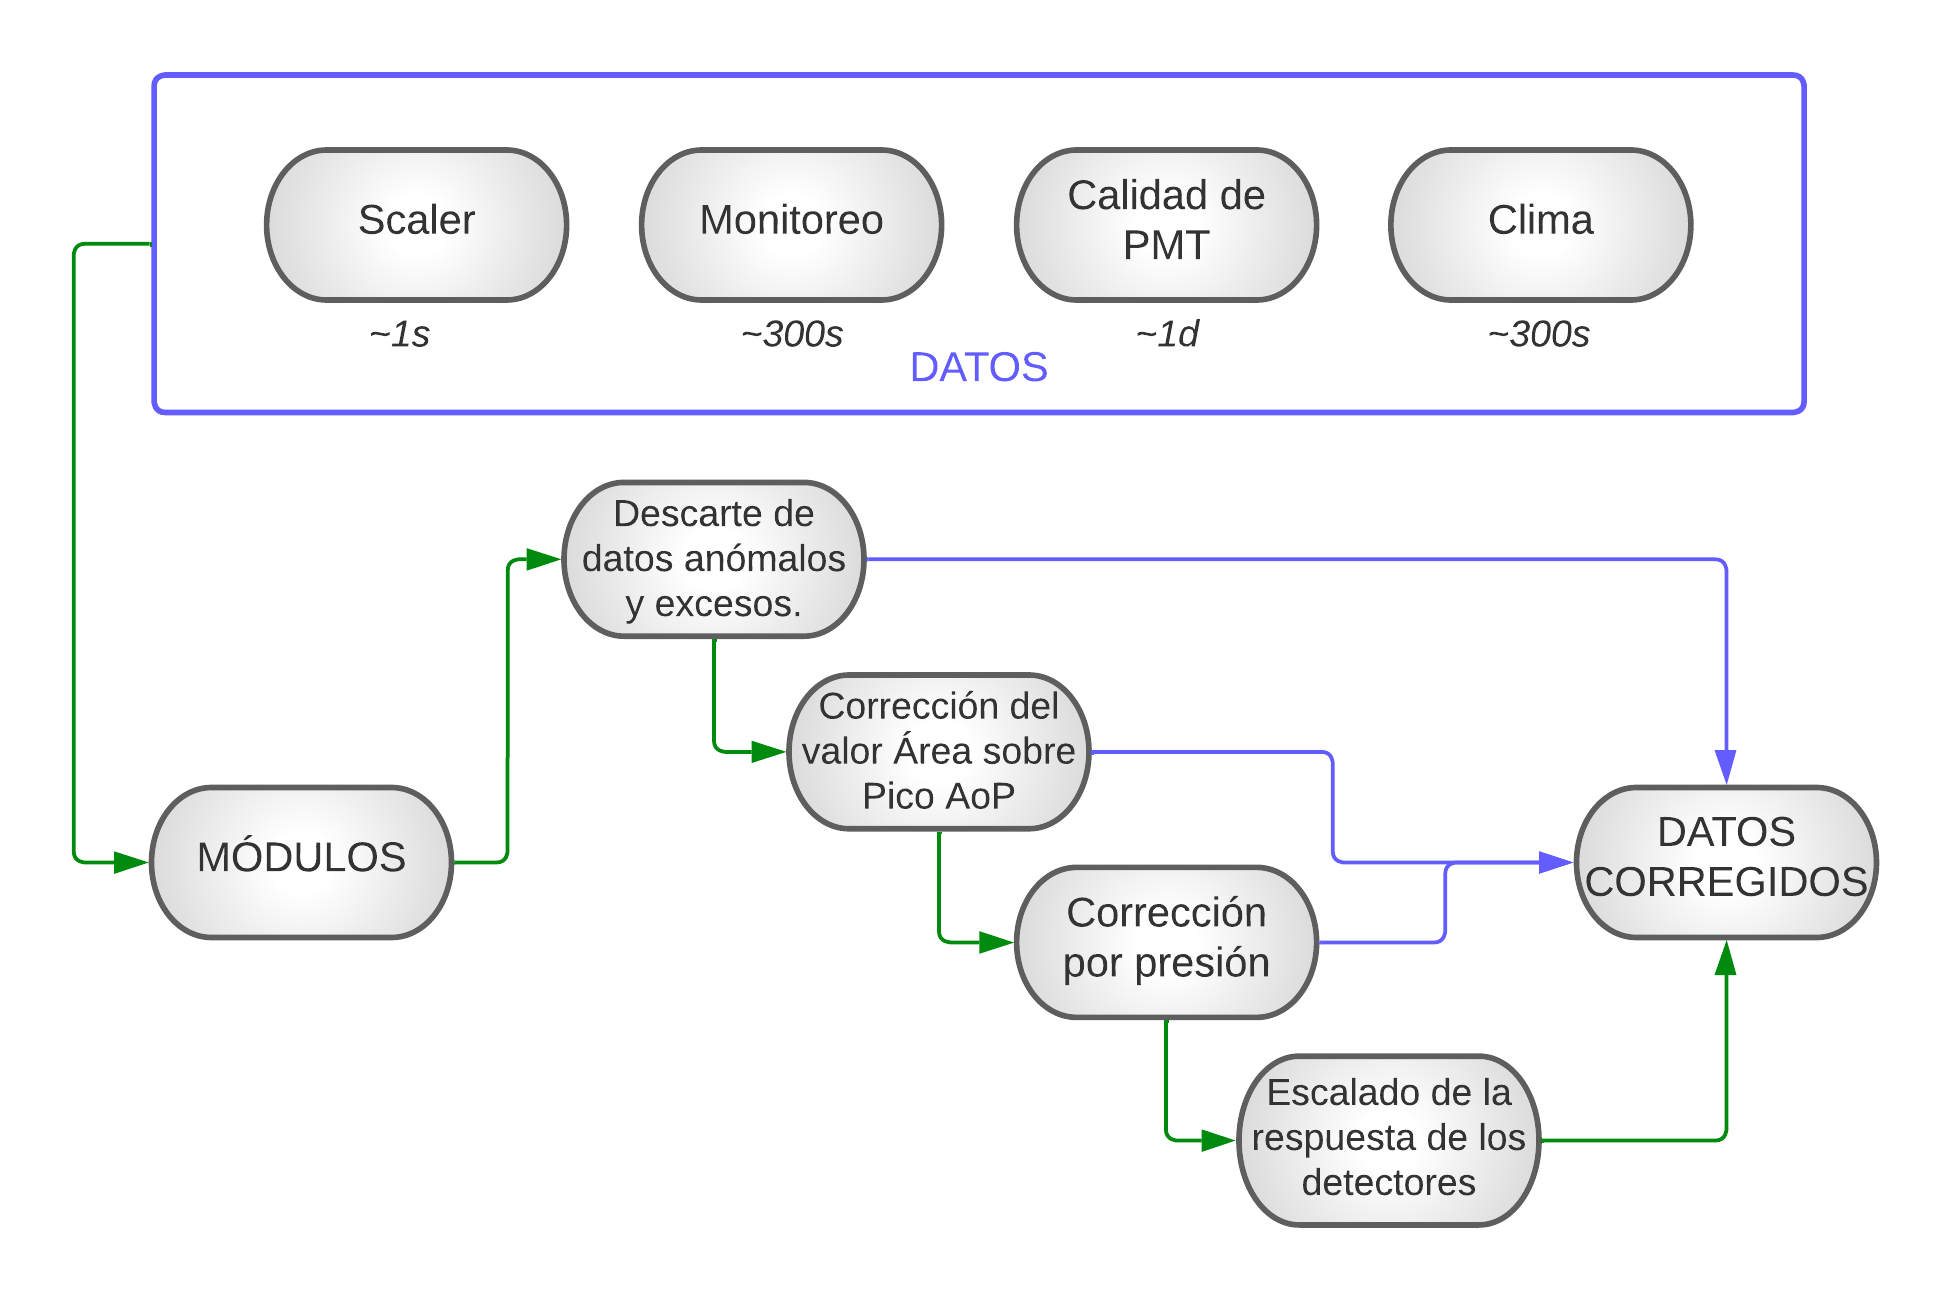
\includegraphics[width=0.7\linewidth]{Figs/SCALER.png}
    \caption{Enter Caption}
    \label{esquema_datos}
\end{figure}
\textbf{Identificación de estaciones erróneas:} Para asegurar la calidad de los datos, solo se seleccionan las estaciones que están configuradas para recoger y transmitir datos válidos cada segundo conforme a los siguientes criterios:
\begin{enumerate}
    \item Estaciones donde los 3 PMT estén en funcionamiento.
    \item Una relación área sobre pico entre $2.5 < AoP < 4.5$ para excluir estaciones que están muy fuera del rango de trabajo normal.
    \item   Estaciones con todos los PMT cumpliendo que $35 < I_{peak}/FADC < 65$. El rango corresponde a una desviación de $\pm30\%$ del valor de diseño tratando de mantener tantas estaciones como sea posible en el análisis.
    \item Se descartan estaciones de las que no se tenga señal de monitoreo.
\end{enumerate}

\textbf{Estaciones atípicas:} Se eliminan las estaciones que notifican tasas de recuento excepcionalmente altas en un solo segundo. Para detectar estos valores atípicos, se utiliza la Desviación Absoluta Mediana (MAD, por sus siglas en inglés). La MAD es una medida de la variabilidad de un conjunto de datos y se define como la mediana de las desviaciones absolutas de los datos con respecto a su mediana. Entonces para cada punto de datos, se calcula cuánto se desvía la mediana del conjunto de datos, se toma el valor absoluto de esa desviación, y luego se obtiene la mediana de todas esas desviaciones. Para cada segundo en la estación, se calcula el valor $z$ que es una medida de cuántas desviaciones estándar puede un dato estar lejos de la media:
\begin{equation}
    z=\frac{\Gamma-\tilde{\Gamma}}{\tilde{\sigma}}
\end{equation}

Donde $\tilde{\Gamma}$ es la mediana y $\tilde{\sigma}$ es la desviación absoluta mediana.  Si  $z>3$ la estación y el segundo se marcan como valores atípicos. En este caso, en lugar de utilizar la media y la desviación estándar, se utilizan la mediana y la MAD, lo que hace que esta medida sea más resistente a los valores atípicos.

\textbf{Rayos y excesos localizados:} Debido al bajo umbral del Scaler, los datos son sensibles a los impulsos electromagnéticos de los rayos, lo que es crucial para el rechazo del ruido de fondo. Se utiliza un método similar a la búsqueda de aumentos de tasa correlacionados con estallidos de rayos gamma para identificar segundos con impactos de rayos. El uso de intervalos de cinco minutos permite una sólida estimación de las tasas medias. Además, un modelo de fondo gaussiano con una señal adicional común facilita la evaluación del exceso de significación, ayudando a marcar los valores atípicos.

\textbf{Promedio y escala:} Se calcula la media aritmética de todos los segundos de cada estación, excluyendo los eliminados por criterios previos. Luego, se obtiene la media de todas las estaciones, enfocándose en el análisis de una sola estación. Esta elección mantiene la claridad conceptual, ya que las correcciones de los efectos a largo plazo se aplican por estación. No se utiliza ninguna ponderación con el número de segundos activos, lo que garantiza la distinción numérica del promedio sobre estaciones por segundo. Para estas correcciones, se utilizan cantidades promediadas como la presión atmosférica y el Área sobre Pico.

\textbf{Correcciones por tendencias a largo plazo:} 

Las tendencias a largo plazo, debidas al envejecimiento de los detectores y a los cambios atmosféricos, requieren correcciones que incluyen: 
\begin{itemize}
    \item Fluctuaciones en la presión atmosférica que corrijan la anticorrelación esperada con la tasa de scaler, esto se puede ajustar con un modelo lineal simple:
\begin{equation}
    \Gamma_{corrected}(t)=\Gamma(t)-a_{1}(p(t)-\langle p\rangle)
\end{equation}
    \item Corrección de área sobre pico (AoP) que se realiza para ajustar los cambios en la forma del pulso en el Detector de Superficie (SD) a lo largo del tiempo. Este ajuste es esencial para estudios a largo plazo, ya que el AoP cambia en una escala de años. El modelo para esta corrección se basa en dos premisas: la señal total disponible (es decir, el número de fotones) en el tanque escala con la calidad óptica del revestimiento acuoso, y la probabilidad de activar todos los tres PMT con una señal de baja energía también escala con la reflectividad del revestimiento. Así, el número esperado de fotoelectrones en el tiempo estaría dado por:
\begin{equation}
    n_{ph}\approx \int s_{ADC}(t|n_{0})  dt  \propto AoP n_{0}
\end{equation}

Donde $s_{ADC}(t|n_{0})$ es la señal integrada en el tiempo en función del número de fotones Cherenkov creados $n_{0}$. 

    \item  Corrección de la línea de base que es el ajuste que se debe realizar para tener en cuenta los cambios constantes en las mediciones de los tubos fotomultiplicadores (PMT), que están correlacionados con la temperatura. Debido a la naturaleza entera de los convertidores analógico-digitales (FADC), y por lo tanto los umbrales del Scaler, esto puede llevar a cambios residuales en la tasa medida.
\end{itemize} 

\section{Detectores de Neutrones vs Pierre Auger}

%(Hatton & Carimichael, 1964)
Los monitores de neutrones (NMs) son una herramienta esencial utilizada en todo el mundo para medir el flujo de partículas secundarias que llegan a la Tierra. Estos detectores terrestres están diseñados para registrar neutrones secundarios generados en lluvias atmosféricas provocadas por iones de rayos cósmicos. Aunque el NM fue inventado por John Simpson en 1958, el diseño estándar que se utiliza actualmente se desarrolló en 1964 (NM64), y se ha convertido en un detector estándar de rayos cósmicos terrestres (\cite{eleana_2017}).

Desde su invención, se ha establecido una extensa red global de estos instrumentos, que abarca desde varias decenas hasta un máximo de 70 estaciones distribuidas en todo el mundo. Los datos recopilados por esta red se utilizan para evaluar las variaciones en el flujo de rayos cósmicos galácticos en el rango de energía de 1 a 100 GeV, proporcionando información crucial sobre el impacto de las tormentas solares, las eyecciones de masa coronal, las estructuras del viento solar y el ciclo de actividad solar en la modulación de los rayos cósmicos (\cite{Ruffolo_2016}).

Los NMs tienen la propiedad de que su dirección de observación barre el espacio con la rotación de la Tierra, por lo que las variaciones diarias (diurnas) en la tasa de recuento de NM proporcionan información adicional sobre la distribución direccional y la anisotropía de los rayos cósmicos (\cite{Ruffolo_2016}). Estos instrumentos utilizan materiales propensos a reacciones nucleares con neutrones, como el litio o el boro.

Debido a que los neutrones son partículas sin carga eléctrica, estos instrumentos se valen de las interacciones posibles de los neutrones energéticos con los núcleos atómicos: colisiones elásticas e inelásticas y reacciones nucleares para producir neutrones rápidos que luego son frenados por un material hidrogenado y medidos indirectamente a través de las partículas ionizantes producidas.

La figura \ref{fig:NM_schem} muestra un diagrama esquemático del monitor de neutrones 6-NM64 ubicado en Atenas, Grecia. El número 6 indica el número de tubos contadores con los que cuenta la estación. La parte b muestra la estructura interna de este detector, en la que se pueden identificar 4 componentes principales: El tubo contador que contiene principalmente $BF_{3}$ (trifluoruro de boro) que al interactuar con los neutrones térmicos producen iones de litio y partículas alfa que al ser acelerados ionizan el gas y producen electrones que provocan una señal que puede ser medida y procesada. Los tubos contadores están recubiertos por una capa moderadora que consta de un tubo de polietileno de 2 cm de espesor que absorbe y refleja los neutrones de evaporación que son generados en el productor de plomo. La capa productora que funciona como blanco de elevada masa atómica, en este caso es plomo, para producir neutrones secundarios y finalmente otra capa reflectora de polietileno (\cite{OlgaMalandraki_2018}).


\begin{figure}
\centering
    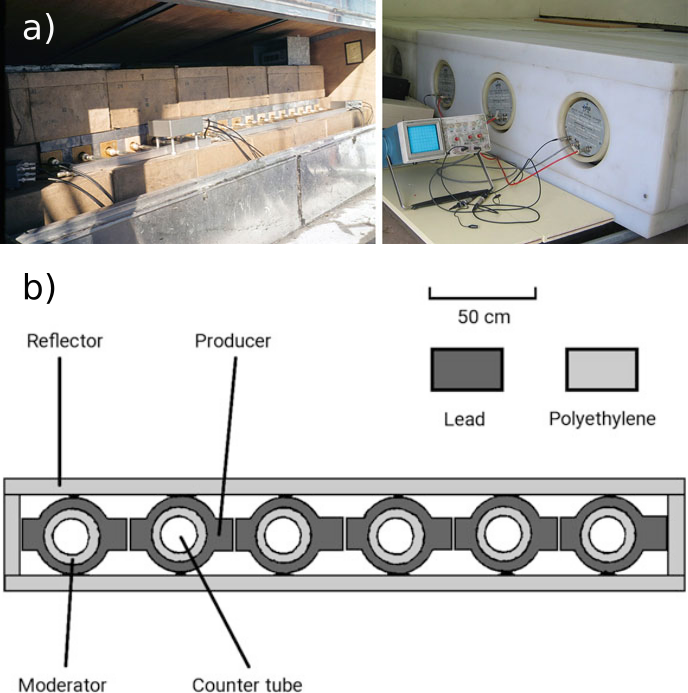
\includegraphics[width=0.7\linewidth]{Figs/NM_schem.png}
    \caption[Diagrama esquemático del monitor de neutrones 6-NM64 ubicado en Atenas, Grecia.]{Diagrama esquemático del monitor de neutrones 6-NM64 ubicado en Atenas, Grecia. El número 6 indica el número de tubos contadores con los que cuenta la estación. La parte b muestra la estructura interna de este detector, en la que se pueden identificar 4 componentes principales: El tubo contador que contiene principalmente $BF_{3}$ (trifluoruro de boro) que al interactuar con los neutrones térmicos producen iones de litio y partículas alfa que al ser acelerados ionizan el gas y producen electrones que provocan una señal que puede ser medida y procesada. Los tubos contadores están recubiertos por una capa moderadora que consta de un tubo de polietileno de 2 cm de espesor que absorbe y refleja los neutrones de evaporación que son generados en el productor de plomo. La capa productora que funciona como blanco de elevada masa atómica, en este caso es plomo, para producir neutrones secundarios y finalmente otra capa reflectora de polietileno. Fuente: \cite{OlgaMalandraki_2018}}
    \label{fig:NM_schem}
\end{figure}
%%%%%%%%%%% BOOOK  Solar Particle Radiation Storms Forecasting and Analysis

%%%%%%%%%%%%%%%%%%%%%%%%%%%
%%%MEJORA REDACCIÓNNNNNN
\begin{comment}
A rasgos generales la tasa de recuento total puede presentarse como una suma de tasas de recuento $N_{i}$ debidas a diferentes especies de GCR:

\begin{equation}
    N = \sum_{i}N_{i} = \sum_{i}\int_{Tci}^\infty J_{i}(T, \phi)Y_{i}(T)dT
\end{equation}
%%%MEJORA REDACCIÓNNNNNN::::
donde Y i es la función de rendimiento específico de NM para la ith especie de GCR, y la integración es sobre la energía cinética por encima de T ci, que es la energía cinética correspondiente a la corte de rigidez geomagnética local Pc y es diferente para diferentes especies de rayos cósmicos. Aquí sólo consideramos las dos especies de RC más abundantes, los protones y las partículas a. Puesto que la contribución de las especies más pesadas es pequeña y su modulación es similar a la de las partículas helio. modulación es similar a la del helio, no las consideramos aquí. aquí. Mientras que la fracción de partículas a es de alrededor del 20$\%$ (en número de nucleones) en LIS, su contribución a la tasa de recuento de NM varía del 23$\%$(NM polar, mínimo solar) al 37$\%$ (NM ecuatorial, máximo solar). (NM ecuatorial, máximo solar) (\cite{Usoskin_2005}).
\end{comment}

Se ha mostrado que el observatorio Pierre Auger funciona también como sensor de las fluctuaciones de los rayos cósmicos galácticos GCR. Sin embargo, como se describió en el capítulo 1, además de las influencias del espacio exterior, la intensidad de los rayos cósmicos observados a nivel del suelo también está determinada por el campo magnético y la atmósfera de la Tierra.  El campo geomagnético desvía las trayectorias de los rayos cósmicos en función de su rigidez de corte, adquiriendo una distribución dependiendo de la ubicación geográfica (\cite{herbst_2013influence}). Esto se traduce en diferencias en las señales medidas por cada una de las estaciones ubicadas alrededor del mundo. 

En la figura \ref{NM_compar} se observa la intensidad de rayos cósmicos normalizada medida para las estaciones de neutrones de Oulu, México, Athenas, Tsumeb comparadas con la tasa de scaler. En la gráfica se observa el comportamiento desde el 2006 hasta el 2021, en donde tenemos todo el ciclo solar 24 (2008-2019). Se observa que todas las estaciones incluido Auger presentan un aumento en el flujo durante los periodos de menor actividad solar y un decremento en la zona de mayor actividad. Observamos también que las estaciones con mayor rigidez de corte presentan una menor variabilidad, sin embargo, la señal del Observatorio Pierre Auger parece estar mucho más atenuada. Indagaremos esto, estimando la sensibilidad que tiene el observatorio ante la actividad solar de corto y largo plazo.
\begin{figure}
\centering
    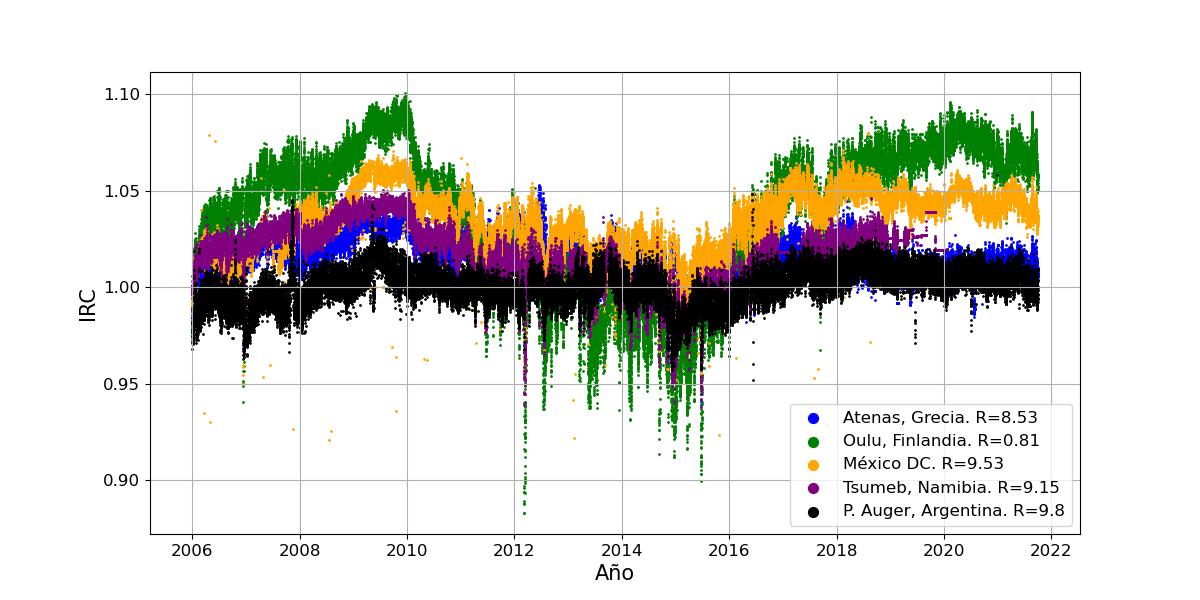
\includegraphics[width=1.1\linewidth]{Figs/Figr/NM_Auger_comparison.png}
    \caption[Diagrama esquemático del monitor de neutrones 6-NM64 ubicado en Atenas, Grecia.]{Intensidad de rayos cósmicos normalizada medida para las estaciones de neutrones de Oulu, México, Athenas, Tsumeb comparadas con la tasa de scaler. En la gráfica se observa el comportamiento desde el 2006 hasta el 2021, en donde tenemos todo el ciclo solar 24 (2008-2019). Se observa que todas las estaciones incluido Auger presentan un aumento en el flujo durante los periodos de menor actividad solar y un decremento en la zona de mayor actividad.  . Elaboración propia}
    \label{NM_compar}
\end{figure}

%%%%%%%%%%%%%%%%%%%%%%%%%%%%%%%%%%%%%%%%%%%%
% TRABAJO CON LOS DATOSSSSSSSSSSSSSSSSSSSSSSSS
Esta comparación se ha realizado considerando que cada dataset, aún corregido puede presentar valores anómalos relacionados a fallas en la detección y inconsistencias en los parámetros de calibración (menos del $1\%$ de los datos). Por esta razón, se aplicó el método de interpolación e imputación para completar los datos faltantes o nulos y generar un series de tiempo consistentes (\cite{wang_2019}).
%%%%%%%%%%%%%%%%%%%%%%%%%%%%%%%%%%%%%
%
%Mediante la figura (xxxx) podems observar perfiles construidos a partir de la técnica de época superpuesta para diferentes observables: La ICME-sheath se muestra con fondo color naranja (intervalo 0 < t < 1), y la ICME con fondo azul (1 < t < 4). El dominio temporal t está normalizado con la duración de la sheath para t < 1, y con la duración de la ICME para t > 1 (la ICME esta representada de tal forma que dura 3 veces más que la sheath, para asemejarse a los casos individuales). Los puntos negros son valores medios para cada bin temporal, los puntos rojos son las medianas asociadas. %%% COLOCAR PIE DE PÁGINA CON LAS EXPLICACIONES MAYBE


\section{Modulación de GCR medido en el Observatorio Pierre Auger}
%%%%%%%%%%%NEWWW
%Verificar cómo hablo de las ICME en el capítulo 1
Una ICME (Eyección de Masa Coronal Interplanetaria) es una gran expulsión de plasma y campo magnético del Sol que se propaga a través del espacio interplanetario. Estas ICMEs pueden influir significativamente en el transporte de los Rayos Cósmicos Galácticos (GCRs) y tienen efectos tanto a nivel local como global en la densidad de GCRs (\cite{Davies_2023}). Estos efectos están relacionados con cambios significativos en las características locales de la turbulencia en el medio interplanetario, así como la presencia de estructuras con líneas de campo magnético suaves e intensas en las nubes que alteran la configuración del viento solar (\cite{Krittinatham_2009}) (Ver capítulo 1).

La Figura \ref{fig:ICME_scaler} realizada en un trabajo previo para Pierre Auger (\cite{masias_2017}), muestra los perfiles superpuestos de los flujos de GCR para diferentes energías en el Observatorio Pierre Auger durante el paso de una ICME. Se observa un aumento en la magnitud del campo magnético interplanetario B, y las fluctuaciones magnéticas rmsB alcanzan su valor máximo en el choque. Las gráficas muestran las desviaciones normalizadas del flujo de scaler, y las dos bandas de histograma. En los datos de scaler se observa una disminución de hasta el −0.3\% a la que le sigue una recuperación similar al efecto observado con los detectores de neutrones. Estos mismos efectos son observados con los modos histograma $H_{sc}$ y $H_{\mu}$ con diferente intensidad llegando a ser hasta de −0.4\%.

Así, durante los periodos de alta actividad solar donde las ICMEs son más frecuentes, van a causar variaciones significativas en los datos del observatorio. Por otro lado, durante los periodos de baja actividad solar, las ICMEs al ser menos frecuentes, y se mantendrán más estables los datos del observatorio.
\begin{figure}
\centering
    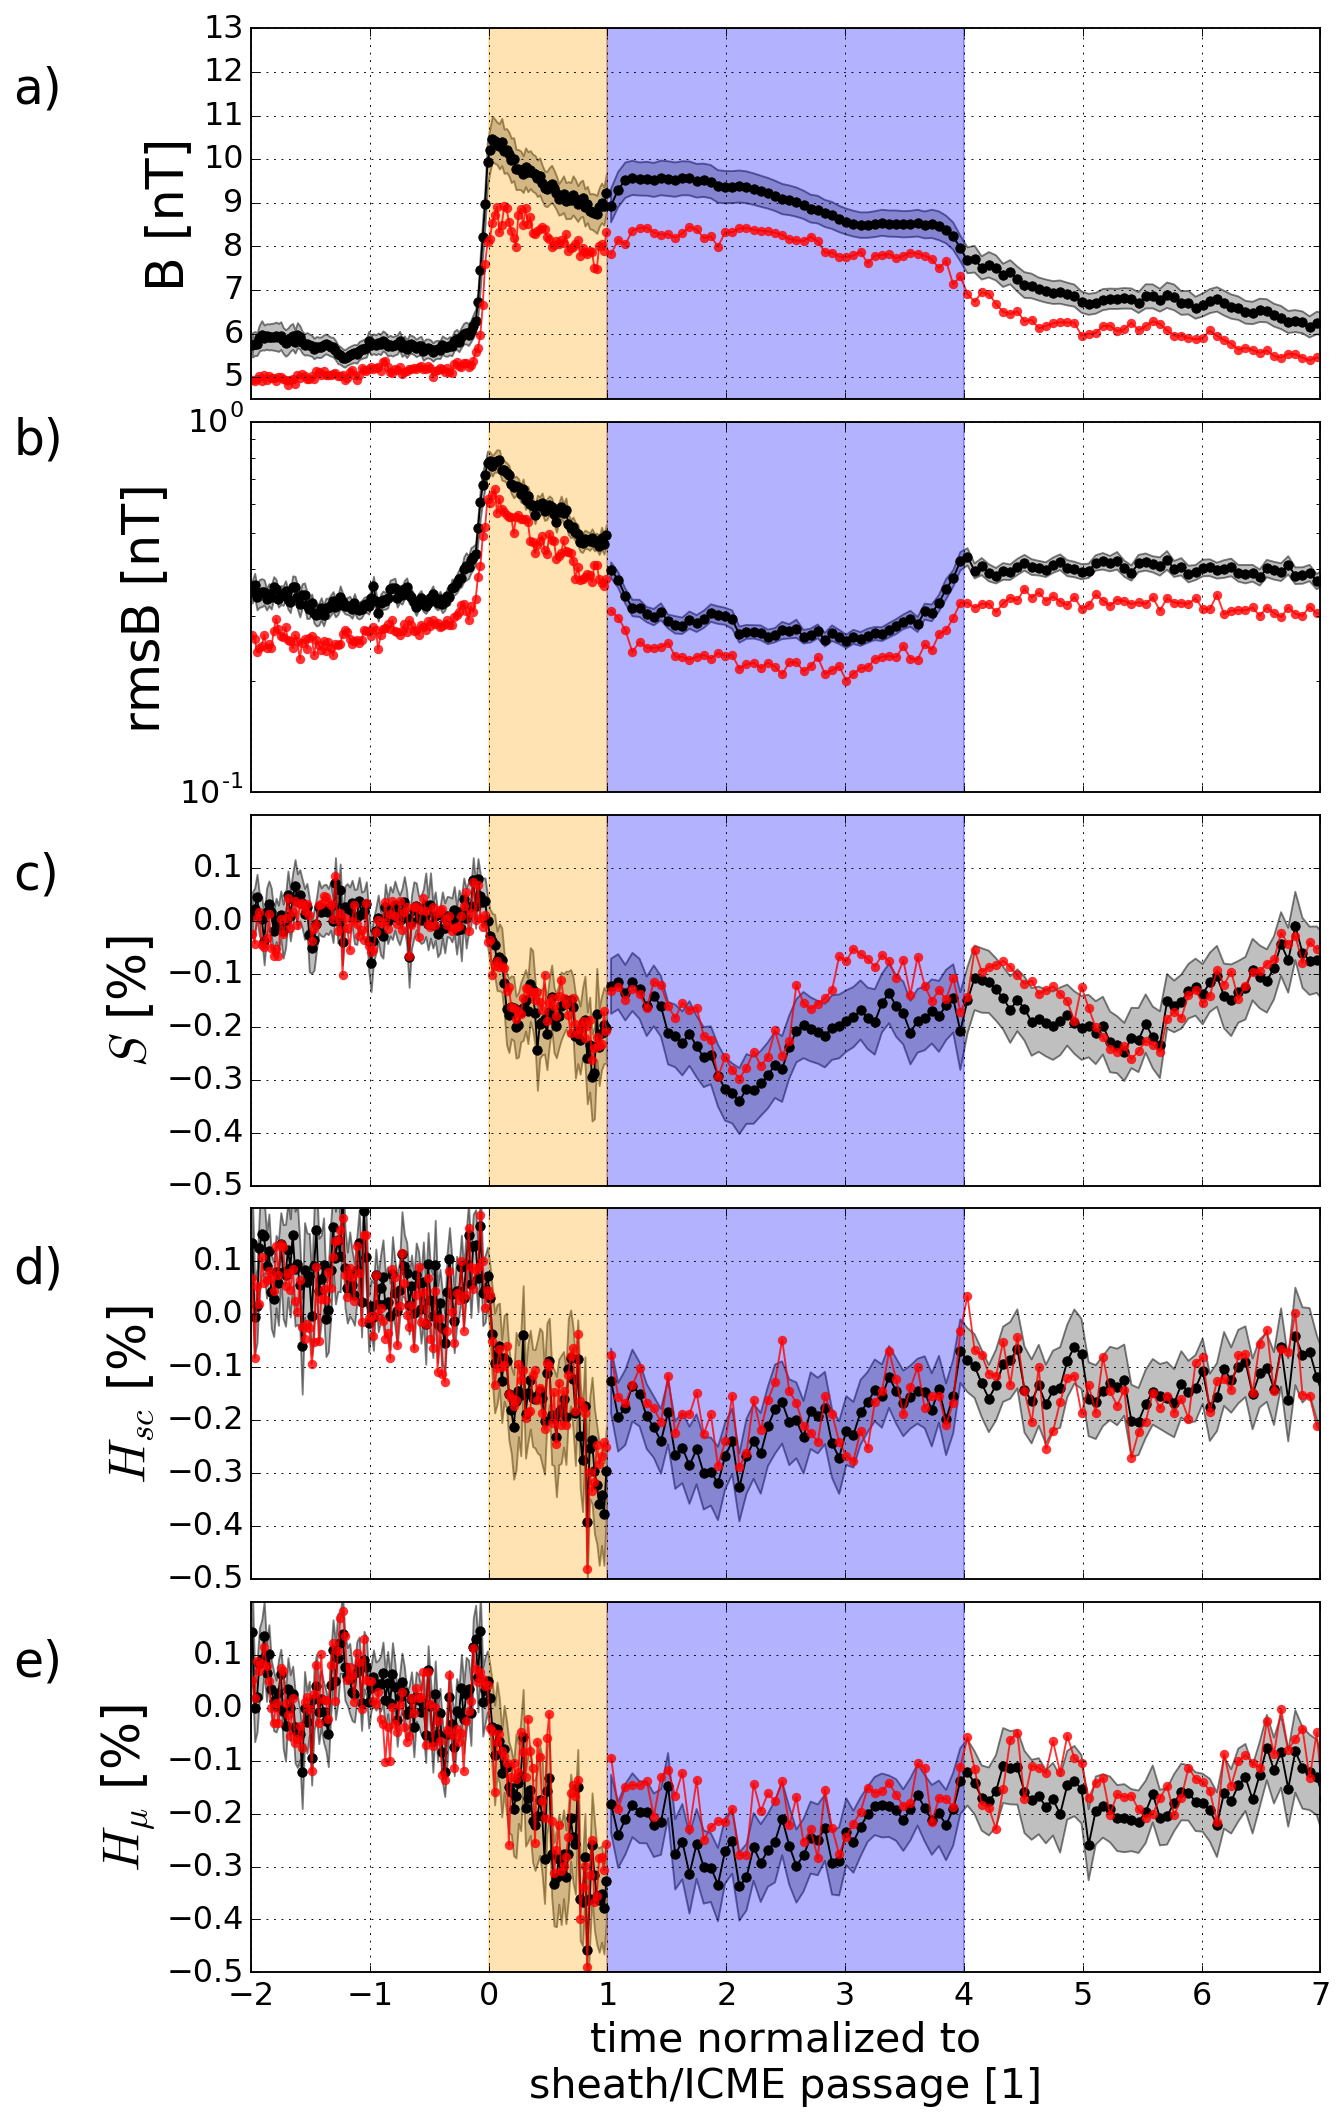
\includegraphics[width=0.7\linewidth]{Figs/ICME_scaler.png}
    \caption{Perfiles superpuestos de los flujos para diferentes energías en el observatorio Pierre Auger en los modos de detección histograma y scaler durante el paso de una ICME en el periodo de funcionamiento del observatorio: La gráfica \textit{a)} muestra un aumento en la magnitud del campo magnético interplanetario B, y la \textit{b)} muestra las fluctuaciones magnéticas rmsB que alcanzan su valor pico en el choque. La gráfica \textit{c)}, \textit{d)} y \textit{e)} muestran las desviaciones normalizadas del flujo de scaler, y las dos bandas de histograma. Fuente: (\cite{masias_2017})}
    \label{fig:ICME_scaler}
\end{figure}
\subsection{Efectos de la periodicidad solar en el fondo de RC medido}

%%%%%%%%%%%  FOURIER DE AUGER Y el NM que escogí
La anterior afirmación puede verse reflejada en la figura \ref{fig:CRIvsSN} donde se ilustran  las distribuciones y tendencias de la intensidad de rayos cósmicos medido, el número de manchas solares (SSN), y la velocidad del viento solar (SWS). La resolución de cada una de estas series de tiempo es de 1 día, y en el caso de la tasa de scaler (medida de la intensidad o flujo de rayos cósmicos secundarios) cuya resolución original es de 300s, hemos realizado un remuestreo a partir del promedio de todos los datos a lo largo de un día, esta técnica la usaremos convenientemente dependiendo de la escala de tiempo en la que nos enfoquemos. Las tendencias (líneas rojas) se determinaron utilizando una media móvil de 15 días (\cite{Oloketuyi_2020}). 

La media móvil es una técnica estadística que usaremos también a lo largo de este estudio, se utiliza con frecuencia para analizar tendencias y suavizar datos. Esta técnica se basa en el Teorema del Límite Central (\cite{Davies_2023}), y consiste en calcular la media de los últimos N valores observados en una serie temporal para minimizar el ruido y mantener una representación precisa de la señal. Los datos, denotados como x(t), pueden considerarse dentro de un marco temporal específico, conocido como ventana deslizante lo que facilita la identificación de las tendencias subyacentes (\cite{wang_2019}). Se puede representar como:
$$
MMS_i = \frac{1}{k} \sum_{j=0}^{k-1} x_{i-j}
$$
De esta forma se suman los $k$ valores más recientes de la serie de tiempo (desde $x_i$ hasta $x_{i-k+1}$), y luego se divide por $k$ para obtener el promedio. Si hay menos de $k$ observaciones disponibles (por ejemplo, al principio de la serie de tiempo), se calcula la media de las observaciones disponibles. Esto significa que si solo tienes $m$ observaciones y $m < k$, la MMS se calcula como:
$$
MMS_i = \frac{1}{m} \sum_{j=0}^{m-1} x_{i-j}
$$
La ventana que escogimos para mostrar la tendencia busca evitar el retardo que se genera en la señal. A partir de la gráfica, , se observa a simple vista una aparente anticorrelación entre la intensidad de rayos cósmicos y el número de manchas solares. Las tendencias revelan claramente las variaciones a largo plazo en respuesta a la actividad solar. Sin embargo no se observa a largo plazo una correlación con la velocidad del viento solar.
%El comportamiento en la CRI podría deberse a la variabilidad de la amplitud del campo magnético heliosférico en el máximo solar, que reduce la afluencia de rayos cósmicos galácticos que entran en el sistema solar, y viceversa en el mínimo solar debido a la baja actividad magnética solar (\cite{Oloketuyi_2020}). Esto indica que el CRI es abundante fuera de la heliosfera, pero su influencia y modulaciones en la heliosfera dependen exclusivamente de las actividades solares.
%cuyo análisis se propone en el trabajo de Oloketuyi y colaboradores
\begin{figure}
    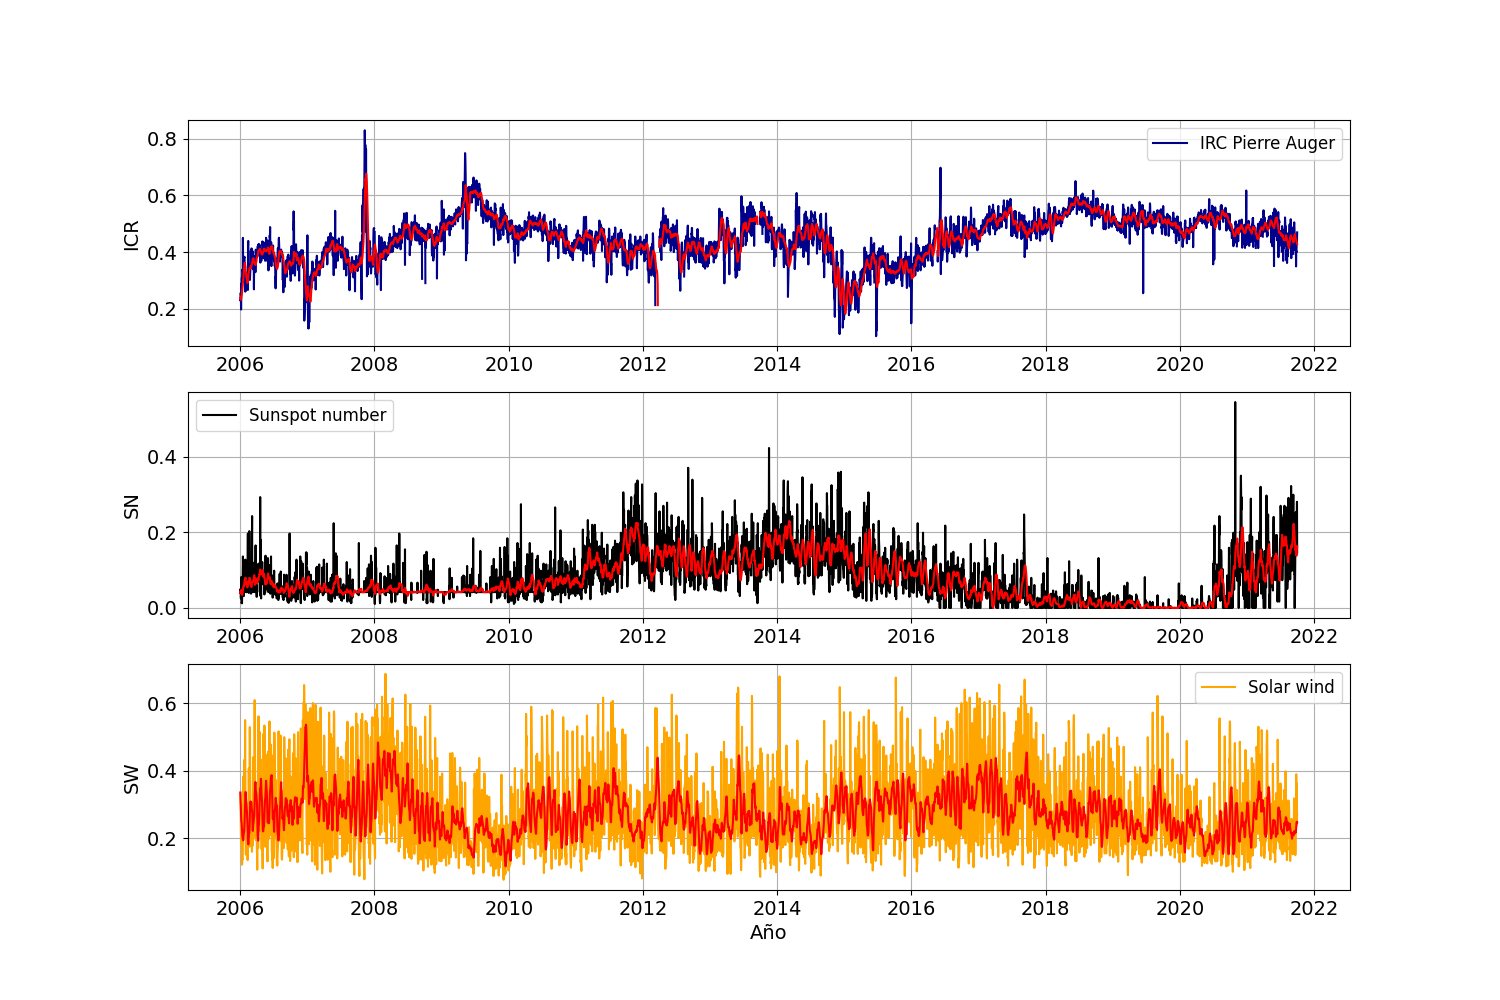
\includegraphics[width=1.1\linewidth]{Figs/Figr/CRI_SN_SW_over.png}
    \caption{Distribuciones y tendencias de SSN (Número de Manchas Solares), CRI (Intensidad de Rayos Cósmicos) y SWS (Velocidad del Viento Solar). Las tendencias se determinaron utilizando una media móvil de 10 días. Se observa una aparente anticorrelación entre el CRI y SSN. Elaboración propia.}
    \label{fig:CRIvsSN}
\end{figure}
Para cuantificar estas observaciones, en la figura \ref{fig:sunspots_corr} se representan los análisis de correlación cruzada entre la Intensidad de Rayos Cósmicos (CRI) el Número de Manchas Solares (SSN) con el  y la Velocidad del Viento Solar (SWS) para los datos del Observatorio Pierre Auger y para las estaciones de neutrones Oulu y Tsumeb. Se escogen estas dos estaciones debido a que Oulu sirve como referencia para la validación de los análisis respecto a otros trabajos (\cite{Oloketuyi_2020}), y Tsumeb por su similitud en el valor de la rigidez de corte geomagnético (\ref{NMs}).

%%%% correlación cruzada
Para calcular la correlación usaremos el método de correlación de Pearson, esta medida estadística evalúa la relación lineal entre dos variables continuas a partir de la obtención de un valor entre 0 y 1. Cuando el coeficiente es cercano a 1, indica una fuerte correlación positiva, es decir, cuando una variable aumenta, la otra también lo hace (\cite{Davies_2023}). Un coeficiente cercano a -1 indica una fuerte correlación negativa, lo que significa que cuando una variable aumenta, la otra disminuye:
$$ r_{xy} = \frac{\sum_{i=1}^{n} (x_i - \bar{x})(y_i - \bar{y})}{\sqrt{\sum_{i=1}^{n} (x_i - \bar{x})^2 \sum_{i=1}^{n} (y_i - \bar{y})^2}} $$
Donde:
- $x_i$ e $y_i$ son los valores individuales de las series $x$ e $y$ respectivamente.
- $\bar{x}$ y $\bar{y}$ son los promedios de las series $x$ e $y$ respectivamente.
- $n$ es el número de observaciones en cada serie.

Este coeficientes es actualmente una medida estándar en estadística por su fácil interpretación, y se ha usado en trabajos precedentes donde también exploran el fondo de rayos cósmicos (\cite{Usoskin_2005}, \cite{Oloketuyi_2020},\cite{Mendonça_2019},\cite{Davies_2023}).
%%% MEJORAR ESTA PARTE CON LA GRÁFICA DE SOLAR WIND
%%%%%
%%%%%%%%%
%%%%%%%%%%%%%%
\begin{figure}
%\centering
    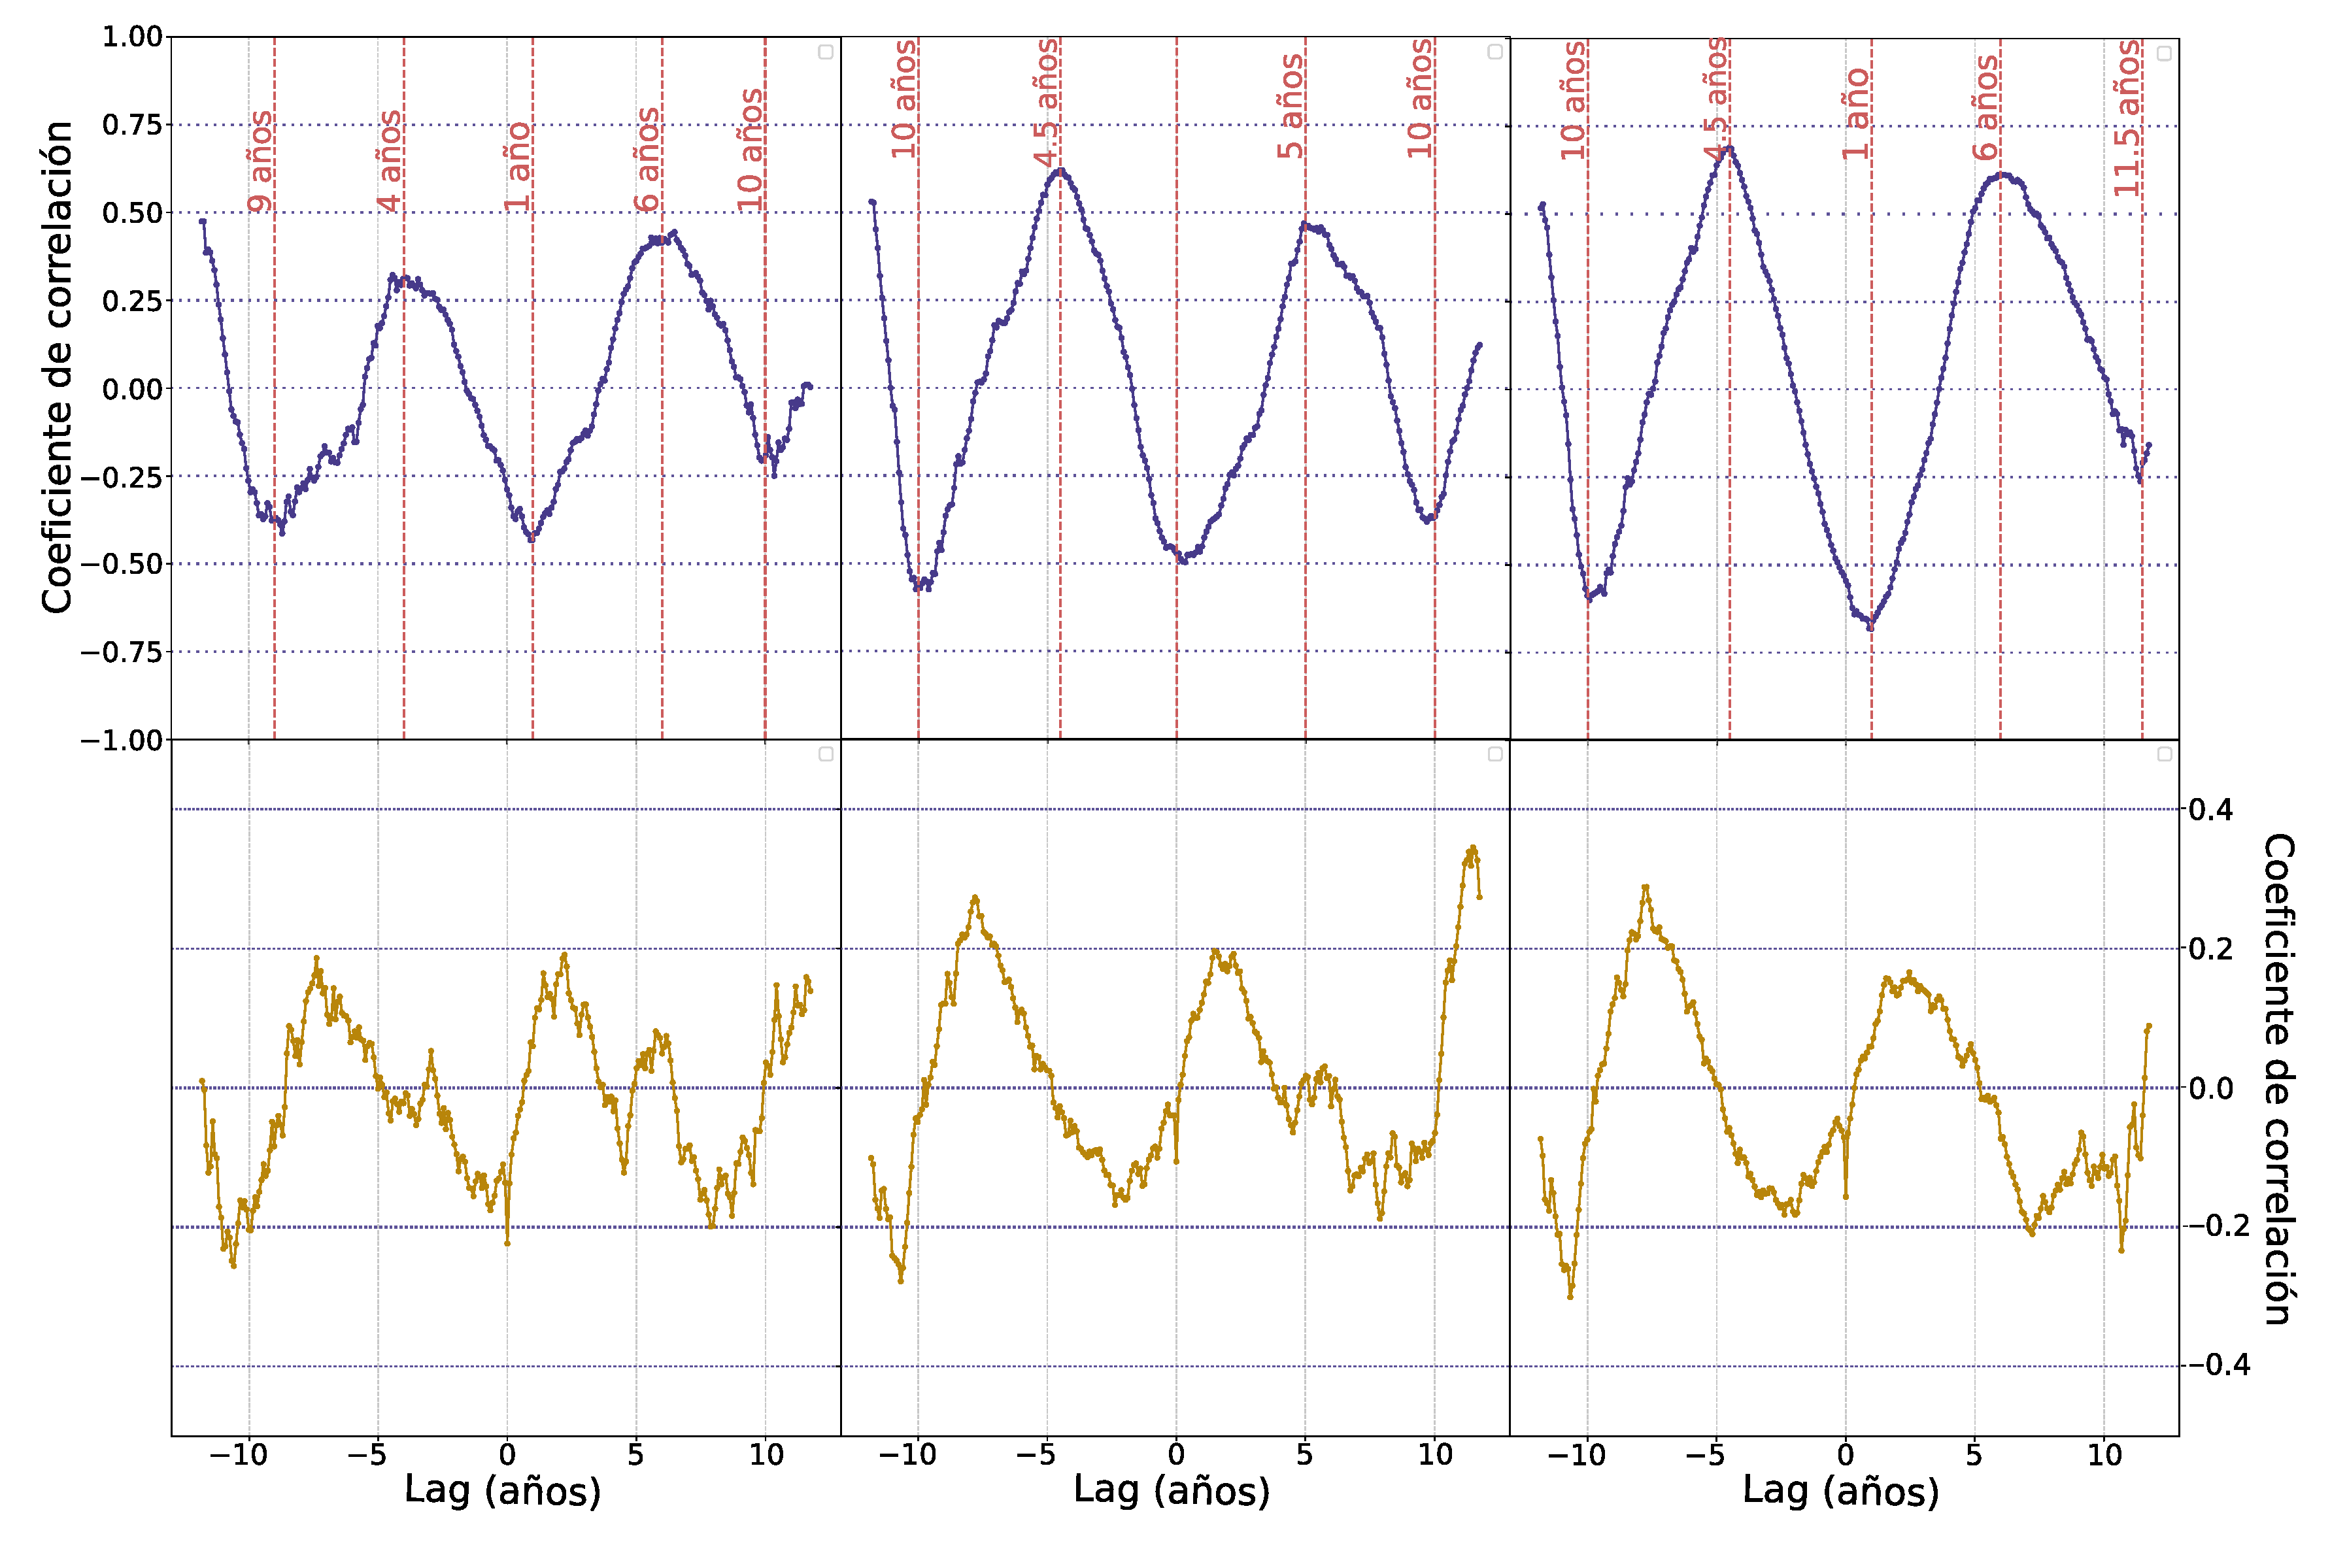
\includegraphics[width=1.0\linewidth]{Figs/Figr/09_cross_correlation.pdf}
    \caption{Análisis de correlación cruzada entre el Número de Manchas Solares (SSN) diario y el Índice de Rayos Cósmicos (CRI) y la Velocidad del Viento Solar (SWS) diarios usando el análisis de correlación cruzada usado en (\cite{Oloketuyi_2020}). El eje x de cada gráfico representa el desfase temporal en relación con el SSN. Los valores negativos indican desplazamientos hacia atrás, mientras que los positivos indican lo contrario, y el valor cero corresponde a la ausencia de desfase. Se observa que el CRI muestra una fuerte correlación negativa con el SSN para el ciclo solar 24. Elaboración propia}
    \label{fig:sunspots_corr}
\end{figure}
El eje x de cada gráfico representa el desfase temporal en relación con el SSN y SW. El signo indica desplazamientos hacia adelante y hacia atrás, y el valor cero corresponde a la ausencia de desfase. Se observa que el CRI muestra una correlación negativa moderada con el SSN para el ciclo solar 24 en Auger y las estaciones de neutrones (entre $0.30$ y $0.50$), y se observa una correlación débil (entre $0.10$ y $0.29$) con el viento solar. Los picos positivos para Auger con valores de 0.30 y 0.48 se ajustan a una correlación moderada positiva en $\approx$5 años, y los tres picos negativos, corresponden a una anticorrelación de 0.45 y 0.58 para un periodo de $\approx$ 8 a 9 años.
%Arreglar para tener la gráfica de correlación con el viento solar.
%Hacer la gráfica comparando el mismo intervalo de tiempo con la estación de neutrones Oulu y México
Es posible cuantificar entonces la sensibilidad del observatorio ante el ciclo solar 24, pero la escala que estamos utilizando nos impide ver los posibles efectos de las otras periodicidades en los datos por ejemplo, $( \thicksim 1, \thicksim13.5,\thicksim27, \thicksim186, \thicksim365$ d). Esto es posible mediante un análisis espectral. Para este trabajo usaremos el método de Blackman-Tukey (\cite{blackman}) aplicado en (\cite{noelia_2023}). El método de Blackman-Tukey es un poderoso enfoque no paramétrico para estimar la \textit{densidad espectral de potencia (PDS)} de series temporales. Éste método produce más del doble de estimaciones de la densidad espectral que la técnica FFT, por lo que las estimaciones B-T tienen una mayor resolución para el mismo coeficiente de variación (\cite{edge_1970}). 
%Este método se basa en el teorema de Wiener-Khinchin, que establece que se puede obtener el espectro de potencia de una serie de tiempo calculando primero su función de autocorrelación y luego aplicando la transformada de Fourier a la función de autocorrelación.
\textbf{Densidad espectral de potencia (PSD):}

La PSD es la medida que especifica los niveles de potencia de los componentes de frecuencia presentes en una señal, así se puede determinar el rango de potencia sobre el cual las frecuencias de la señal están operando. A partir del teorema de Wiener-Khinchin, se define como la transformada de Fourier de la la función de autocorrelación de una señal. Cuando se presenta un proceso aleatorio, la transformada de Fourier no puede ser aplicada directamente debido a que la mayoría de las realizaciones tienen formas irregulares y no pueden presentarse analíticamente (\cite{HerreraSepulveda_2017}). En estos casos solución para este inconveniente es entonces la aplicación de la función de autocorrelación . Esta función se define como el valor esperado de las variables aleatorias del proceso en los instantes de tiempo $t_1$ y $t_2$:
\begin{equation}
    R_{xx}(t_1 t_2) = E{X(t_1)X(t_2)}
\end{equation}
Si el proceso aleatorio es estacionario, la función de autocorrelación solo depende de la diferencia de los tiempos $(\tau)$:
\begin{equation}
    R_{xx}(\tau) = E{X(t)X(t+\tau)}
\end{equation}
Ahora bien, la densidad espectral de potencia PSD está dada por:
\begin{equation}
   S_{xx}(\omega) = \int_{-\infty}^{\infty} R_{xx}(\tau) e^{-j\omega\tau} d\tau
\end{equation}
Existen dos técnicas principales para estimar la Densidad Espectral de Potencia (DEP): el método paramétrico y el no paramétrico. El método paramétrico utiliza un modelo para el proceso aleatorio para estimar el espectro de potencia, incluyendo técnicas como el modelo de media móvil (MA), el modelo autoregresivo (AR) y el modelo autoregresivo de media móvil (ARMA). Por otro lado, el método no paramétrico estima primero la secuencia de autocorrelación de un conjunto de datos y luego estima el espectro de potencia a través de la Transformada de Fourier de la secuencia de autocorrelación estimada, utilizando técnicas como el periodograma, el método de Barlett, el método de Welch y el método de Blackman-Tukey (\cite{HerreraSepulveda_2017}).
\begin{comment}
    Suponiendo que tras las correcciones por presión y temperatura no haya más variables atmosféricas que afecten a la tasa de recuento, un análisis espectral proporcionará periodicidades relacionadas con los efectos heliosféricos. Existen varias técnicas para realizar una estimación de la densidad espectral de potencia (PDS). Entre los métodos no paramétricos se encuentra el método de Blackman-Tukey (Blackman & Tukey, 1958). Este método se basa en el hecho de que la transformada de Fourier de una función de autocorrelación de una serie temporal es equivalente a su espectro de potencia. Ponderar la función de autocorrelación según diversas formas es un método tradicional para reducir una fuga de potencia. Estimamos la PSD de la S 00 horaria aplicando el método de Blackman-Tukey y considerando la ventana de Hanning de un tamaño igual a 0,3 de la longitud de los datos. Para determinar la importancia de los picos espectrales, se ha empleado la generación de un espectro de ruido rojo. Los picos espectrales que tienen amplitudes superiores al intervalo de confianza del 95 % se distinguen estadísticamente del espectro de ruido rojo de fondo.
\end{comment}
La gráfica \ref{FFT} muestra la expansión discreta en serie de Fourier del flujo de CR medido en el observatorio en escala logarítmica. Los datos se reescalaron a tres horas de tal forma que la señal diurna pueda ser observada. Los picos más agudos en la potencia espectral son visibles para una señal con una componente diaria, mensual y anual que se pronuncian al realizar un suavizado de ventana móvil a la densidad espectral de potencia como se muestra en la gráfica de la derecha. 

La señal diurna está relacionada a la rotación de la Tierra, su interacción con el viento solar magnetizado y la anisotropía espacial del flujo de GCR. Esta fluctuación diaria está causada por un equilibrio entre la convección radial del viento solar hacia el exterior de los GCR y la difusión hacia el interior a lo largo del campo magnético interplanetario (IMF) (\cite{martin_ICRC} \cite{noelia_2023}). 

La componente mensual con un periodo de 27 días está relacionada a la rotación de Carrington (\cite{martin_ICRC}) y es ocasionada por la combinación de la rotación solar con una distribución desigual de las zonas activas solares de larga duración, como las manchas solares, los agujeros coronales, las CME y las zonas de interacción corrotantes. Estos fenómenos generan condiciones electromagnéticas longitudinalmente asimétricas de la heliosfera durante una única revolución solar (\cite{grieder_2001}). El periodo rotacional, causado por la rotación diferencial solar, es de unos 25 días en la zona casi ecuatorial y de 38 días en los polos.

La rotación de la Tierra alrededor del Sol, que influye en el flujo de GCR, es la causa principal de la fluctuación anual del periodo de 365,25 días en los datos scaler. El flujo de GCR disminuye en el afelio, cuando la Tierra está más lejos del Sol, y aumenta en el perihelio, cuando está más cerca del Sol. En esta investigación, este fenómeno no se estudió a profundidad pero las observaciones de esta modulación han sido reportadas en trabajos previos (\cite{grieder_2001}).
\begin{figure}
\centering
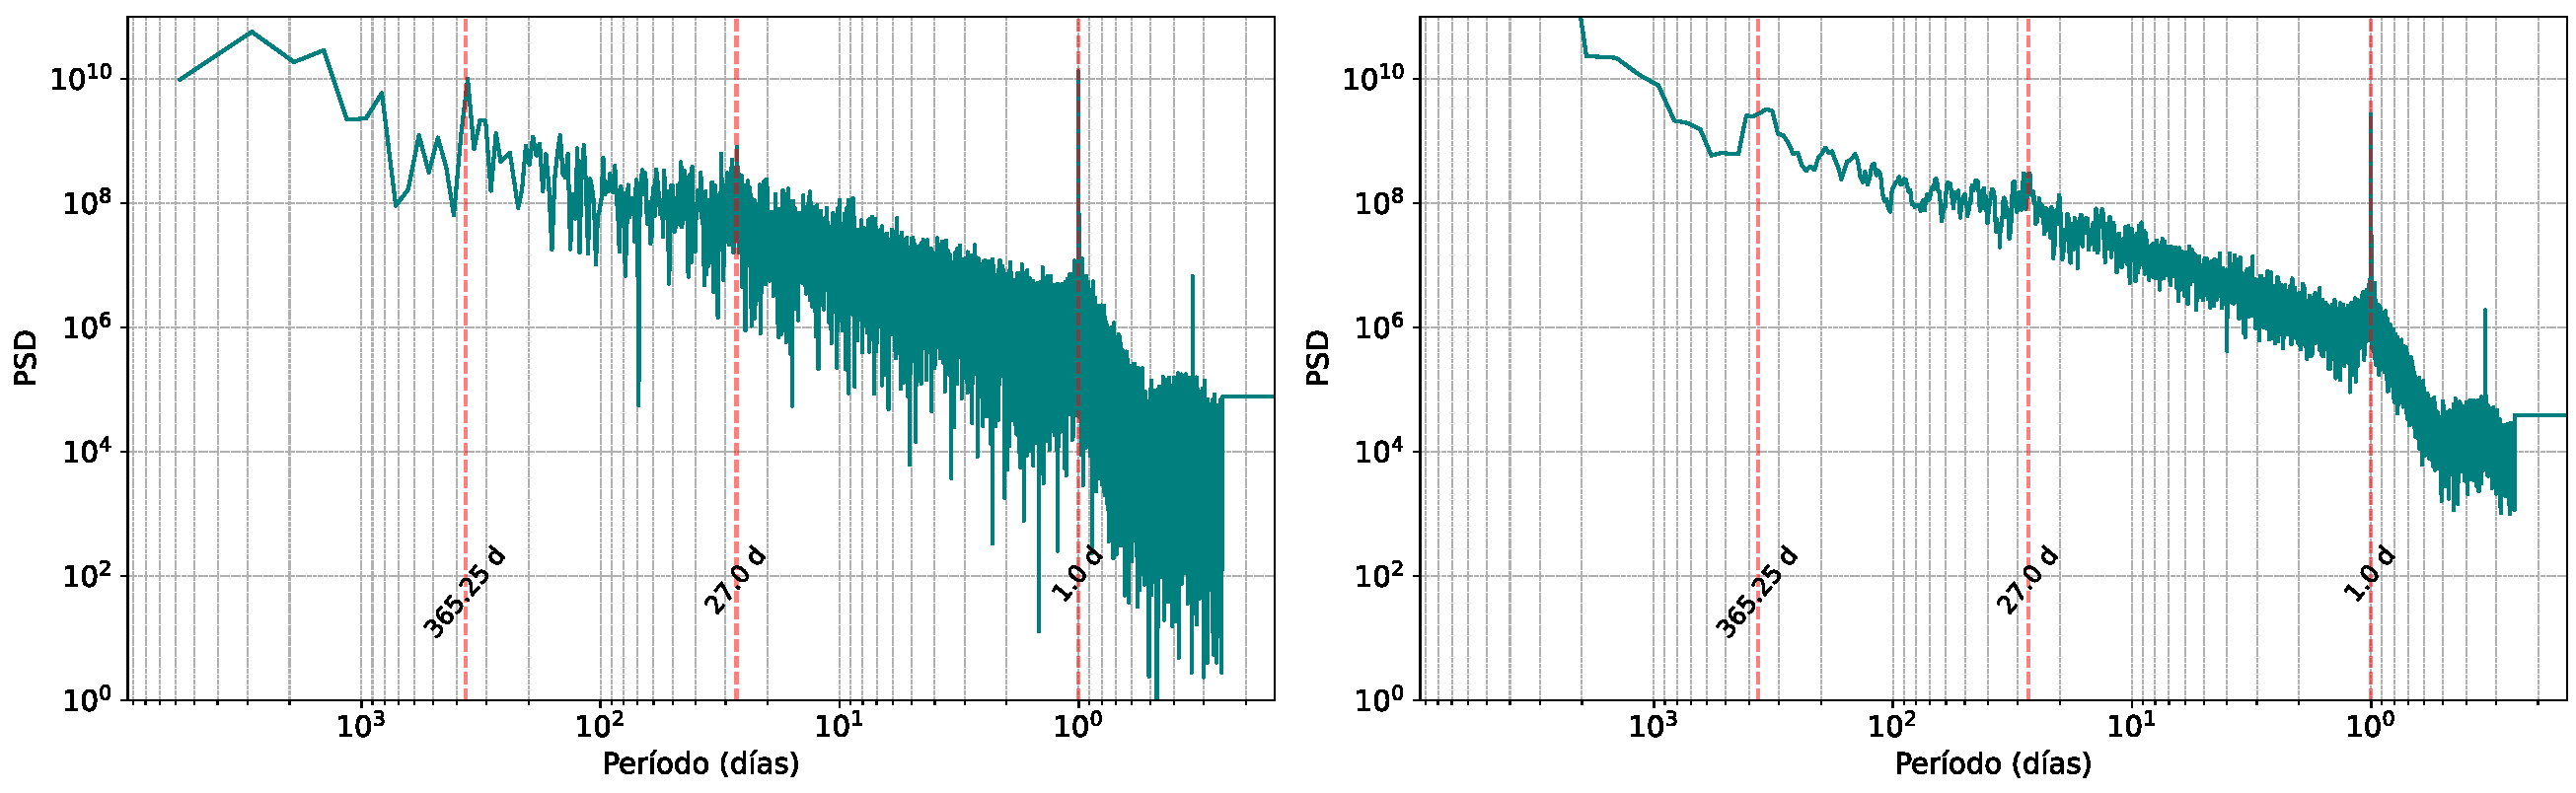
\includegraphics[width=1\linewidth]{Figs/Figr/12_PSD_total.pdf}
    \caption{Pendiente modificar con Autocorrelación para eliminar el ruido.}
    \label{FFT1}
\end{figure}
\subsection{Sensibilidad a eventos transitorios y de corto plazo}
%%%%% BÚSQUEDA DE FORBUSH
La resolución temporal de la tasa de scaler de 300s puede utilizarse para la búsqueda de eventos transitorios como los Forbush Decrease cuya presencia en los datos del Observatorio ya ha sido reportada. El presente trabajo no busca identificar los eventos, sino caracterizar la sensibilidad del Observatorio ante FE (Eventos Forbush) de diferentes intensidades. Para ello, vamos a usar la información del catálogo de eventos Forbush y disturbios interplanetarios como se describe en la sección 3.1, en los periodos 2006 -2019 estableciendo criterios físicos para la selección de eventos significativos. La gráfica \ref{fig:FD_events} muestra todas las magnitudes de los FE registrados en la base de datos, clasificados por la fuente que lo ha generado. Se observa que la mayor cantidad de eventos son aquellos que no tienen una relación confirmada  con fenómenos solares transitorios (puntos azules). No obstante, estos FE tienen en su mayoría magnitudes muy bajas y no presentan un comportamiento fuertemente ligado al ciclo solar, como sí se observa en los eventos asociados a Ondas de Choque Interplanetario OCI y comienzos de tormentas súbitas SSC. Especialmente estos eventos son los que presentan una mayor magnitud.
\begin{figure}
\centering
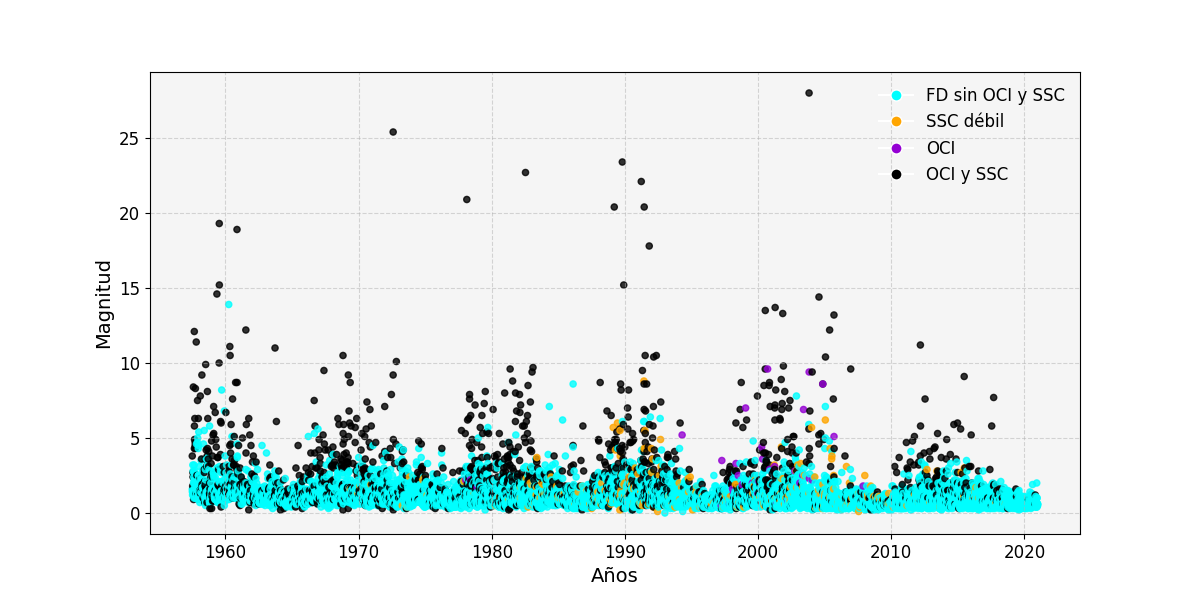
\includegraphics[width=1.2\linewidth]{Figs/Figr/forbush_events.png}
    \caption{Magnitudes de los FE registrados en la base de datos, clasificados por la fuente que lo ha generado. }
    \label{fig:FD_events}
\end{figure}
Se seleccionaron los FE que cumplieran con las siguientes características en la base de datos:
\begin{itemize}
    \item Eventos cuyas fuentes son Ondas de Choque Interplanetarias OCI y Comienzos de tormenta súbita SSC (OType = 1).
    \item Alta confiabilidad en la asociación del FE con la fuente (Qs = 4 y 5).
\end{itemize}
En total son 148 FE que cumplen con estas características para el periodo de tiempo de funcionamiento del observatorio, la tabla (\ref{tabla_FE_Auger}) muestra la lista de eventos seleccionados con algunos parámetros de interés como la fecha y hora del evento solar con el que está asociado, el tipo de fuente y la magnitud.
%%%%%%%%%%%%%%%%   TABLAAAAAAAAAAAA FORBUSHHHH
%%%%%%%%%%%%%%%%
La gráfica \ref{hist_FE} muestra un histograma que representa los eventos forbush  en relación a su magnitud, 
que es la variación máxima de la densidad CR provocada. La magnitud (MagnM corregida por efectos magnetosféricos) será nuestro parámetro principal para este análisis puesto que se ha cuantificado la relación estadística entre la rigidez geomagnética y la magnitud de la FE (\cite{belov_2009}), a pesar de que esto sigue siendo a la fecha un problema que necesita seguir siendo estudiado y se aborda más recientemente por Wang y colaboradores  donde han definido la amplitud de un FD y la rigidez máxima afectada, valor para hasta el cual los efectos de los FE siguen siendo significativos (\cite{wang_2023}). En general, valores bajos de FE $(<1\%)$ suelen indicar condiciones geomagnéticas tranquilas e inestables y los masivos suelen seguir a tormentas magnéticas excepcionalmente grandes, como las ocurridas en agosto de 1972, julio de 1982 y octubre de 2003 (\cite{belov_2009}).  De las 16 tormentas magnéticas con un Kp máximo de 9, 13 tuvieron fluctuaciones de electrones superiores al $5\%$ después de ellas. En un periodo de 50 años, las tormentas geomagnéticas intensas siguieron a la mitad de las diez mayores fluctuaciones de electrones, mientras que las tormentas severas o fuertes siguieron a la otra mitad y este comportamiento que podemos asociar al ciclo solar de 11 años, se ve reflejado en la figura \ref{fig:FD_events}.
\begin{figure}
    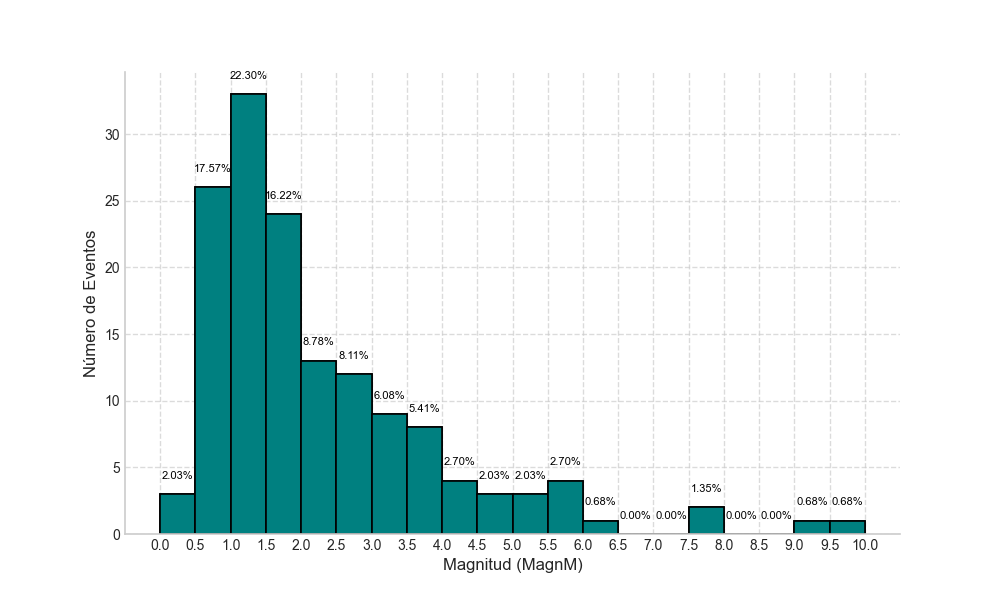
\includegraphics[width=1\linewidth]{Figs/Figr/CRI_FD_HISTOGRAMA.png}
    \caption{Enter Caption}
    \label{hist_FE}
\end{figure}
De igual forma observamos a través del histograma de la figura \ref{hist_FE} que la mayor cantidad de eventos tiene magnitud por debajo del ($2\%$). Este porcentaje representa el $60.14\%$ de del total de FE en la base de datos y el $58.39\%$ de los eventos en el periodo 2006-2021 manteniéndose la tendencia. Enfocándonos en la ventana correspondiende al periodo accesible para los datos del Observatorio, a través de la figura \ref{fig:FD_scaler} podemos visualizar la magnitud normalizada de FE entre 2006 a 2021 a la vez junto con la tasa de scaler normalizada. La barra de color en la parte superior divide el eje x en 15 secciones correspondiente a cada año  y el color representa el número de eventos registrados en cada año.
%Se observa una relación estadística entre el grado de actividad geomagnética y la magnitud de la FE. Valores bajos de FE (<1%) suelen indicar condiciones geomagnéticas tranquilas e inestables. Por el contrario, los FE masivos suelen seguir a tormentas magnéticas excepcionalmente grandes, como demuestran las ocurridas en agosto de 1972, julio de 1982 y octubre de 2003. Trece de las dieciséis tormentas magnéticas con un Kp máximo = 9 tuvieron FEs >5% tras ellas. Por otra parte, las tormentas geomagnéticas intensas siguieron a la mitad de las diez mayores FE durante un periodo de 50 años, mientras que las tormentas severas o fuertes siguieron a la otra mitad.
Según la gráfica la mayor cantidad de FE ($55.41\%$) se encuentran en la zona de máxima actividad solar (2012-2016) en esta región,  se encuentra el $71.20\%$ de los eventos con magnitud $>2\%$ respecto a todo el periodo de registro del observatorio sirviendo como validación respecto a las observaciones de Belov y colaboradores (\cite{belov_2009}).
\begin{figure}
    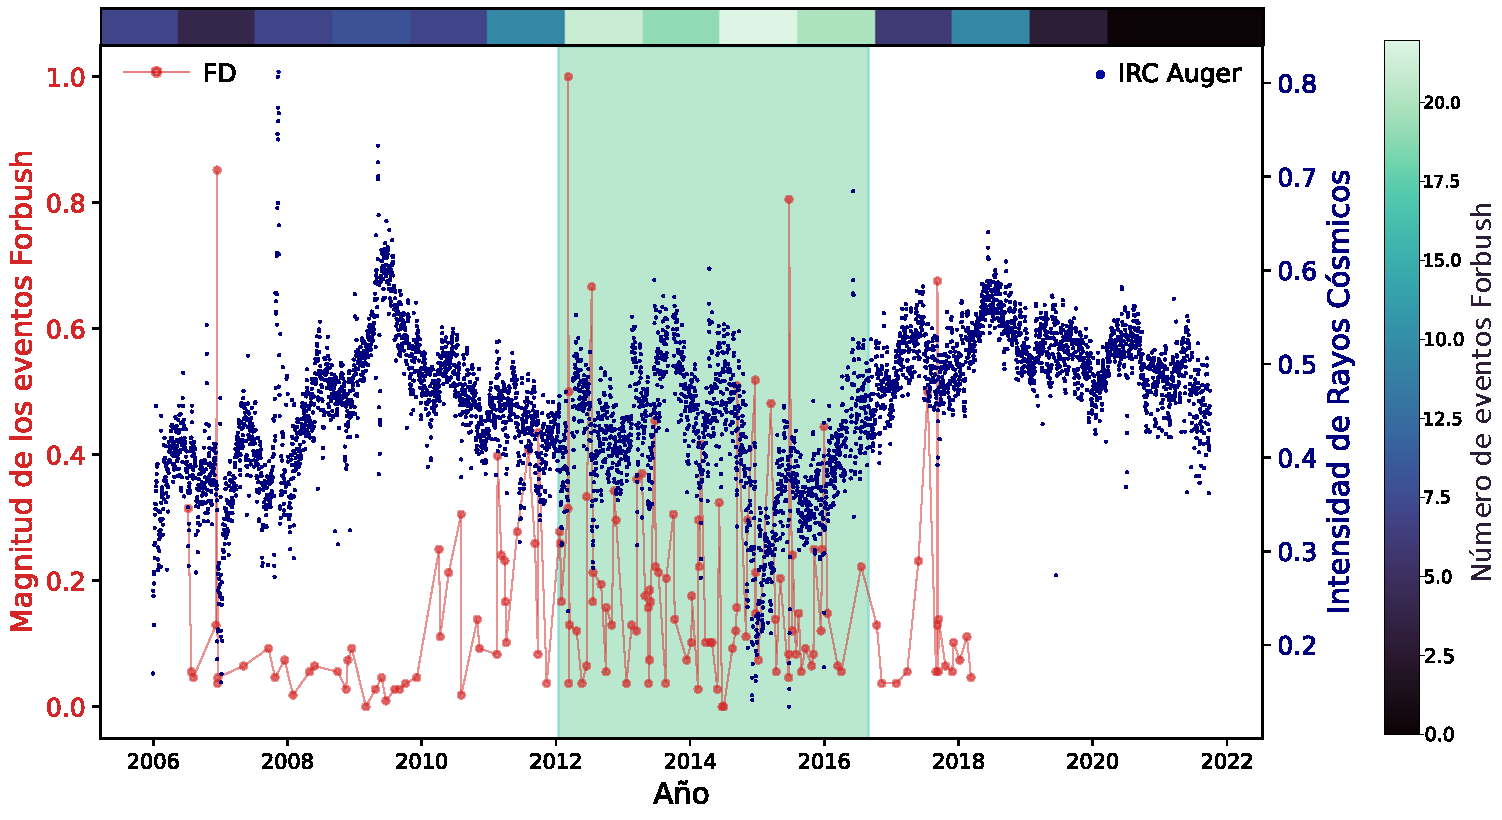
\includegraphics[width=1\linewidth]{Figs/Figr/FD_Scaler_AUGER.pdf}
    \caption{Enter Caption}
    \label{fig:FD_scaler}
\end{figure}
%ESTO VA ARRIBA EN LA PERIODICIDAD DIARIA
%En el trabajo de \cite{martin_ICRC} realizado también para el Observatorio Pierre Auger se reporta un comportamiento
%Lo anterior confirma la hipótesis que asocia las irregularidades en los perfiles de scaler diarios en el periodo de tiempo de máxima actividad solar con una mayor tasa de FE.
Veamos cómo se comportan los scaler a cortas escalas, más específicamente en el rango de la duración habitual de un FE (días). Para esto es importante resaltar que como se ha mostrado a lo largo de este capítulo, el flujo de fondo de RC es muy sensible a fluctuaciones de diferentes frecuencias causadas por la actividad solar y esto supone un desafío a la hora de aplicar técnicas de filtrado que eliminen el ruido. Identificar eventos transitorios implica caracterizar muy bien el ruido de la señal medida por el observatorio. En este caso el ruido no solo comprende las fluctuaciones aleatorias de la señal sino también las frecuencias asociadas a la modulación periódica a diferentes escalas causadas por el Sol. Sin embargo las técnicas de filtrado como la ventana móvil pueden ser útiles para suavizar la señal y hacer nuestra caracterización de Forbush.

Como primera aproximación, vamos a realizar un filtrado únicamente de la modulación diaria a partir del método de la ventana móvil. Este método es especialmente útil para eliminar el ruido de alta frecuencia de una señal (\cite{Davies_2023}). La figura \ref{1d_filter} muestra los datos disponibles para el tiempo de funcionamiento del Observatorio con una taza de muestreo de 300s contrastando las señales con y sin filtro. Adicionalmente mediante  la figura \ref{filter_result} podemos observar una escala mucho menor en la que se muestra un FE ocurrido el 22 de junio del 2015 de magnitud $9.6\%$. Este FE es el más intenso medido por el observatorio y es de especial interés ya que fue generado por la segunda mayor tormenta geomagnética del ciclo solar 24. 

Esta tormenta fue generada por dos llamaradas solares clase M el 21 de junio del 2015 dando lugar a una CME, que demoró unas 39,5 horas en llegar.  La rápida velocidad inicial de la CME, la desviación por los agujeros coronales y la consiguiente reducción de su velocidad hacia la Tierra contribuyeron a que llegara a la Tierra antes de lo esperado (\cite{golpsdwamy_2018}). Adicionalmente, este  y otros FE significativos fueron utilizados para hacer una diferenciación entre FE generados por IMCE o por Regiones de Interacción Corrotantes (CIRs por sus siglas en inglés), que son regiones de interacción que se forman entre corrientes de viento solar de alta velocidad y corrientes lentas, lo que lleva a campos magnéticos y plasmas comprimidos, estudio que contribuyó recientemente en la comprensión de la relación entre la magnitud de los FE y la rigidez de corte geomagnético reportado en (\cite{wang_2023}).


\begin{figure}
\centering
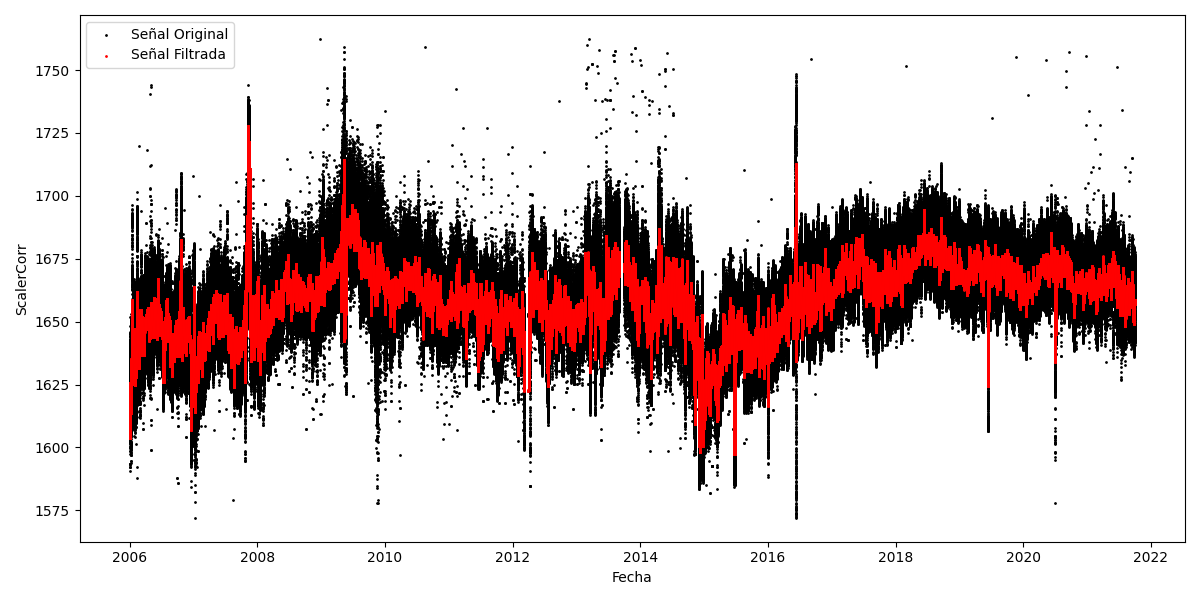
\includegraphics[width=1\linewidth]{Figs/Figr/auger_filter_1D.png}
    \caption{Pendiente modificar con Autocorrelación para eliminar el ruido.}
    \label{1d_filter}
\end{figure}
%Para ello, vamos a remover periodicidad diaria de los datos que interfieren con la identificación de estos eventos
%\ref{FD1} podemos observar un Forbush con magnitud 9.5 medido por los scaler con la señal sin filtrar y con la señal filtrada. El suavizado para eliminar la priodicidad diaria se realiza con la ventana móvil de un día. ¿Cuál es entonces la mínima sensibilidad que tiene el observatorio a estos eventos?
\begin{figure}
\centering
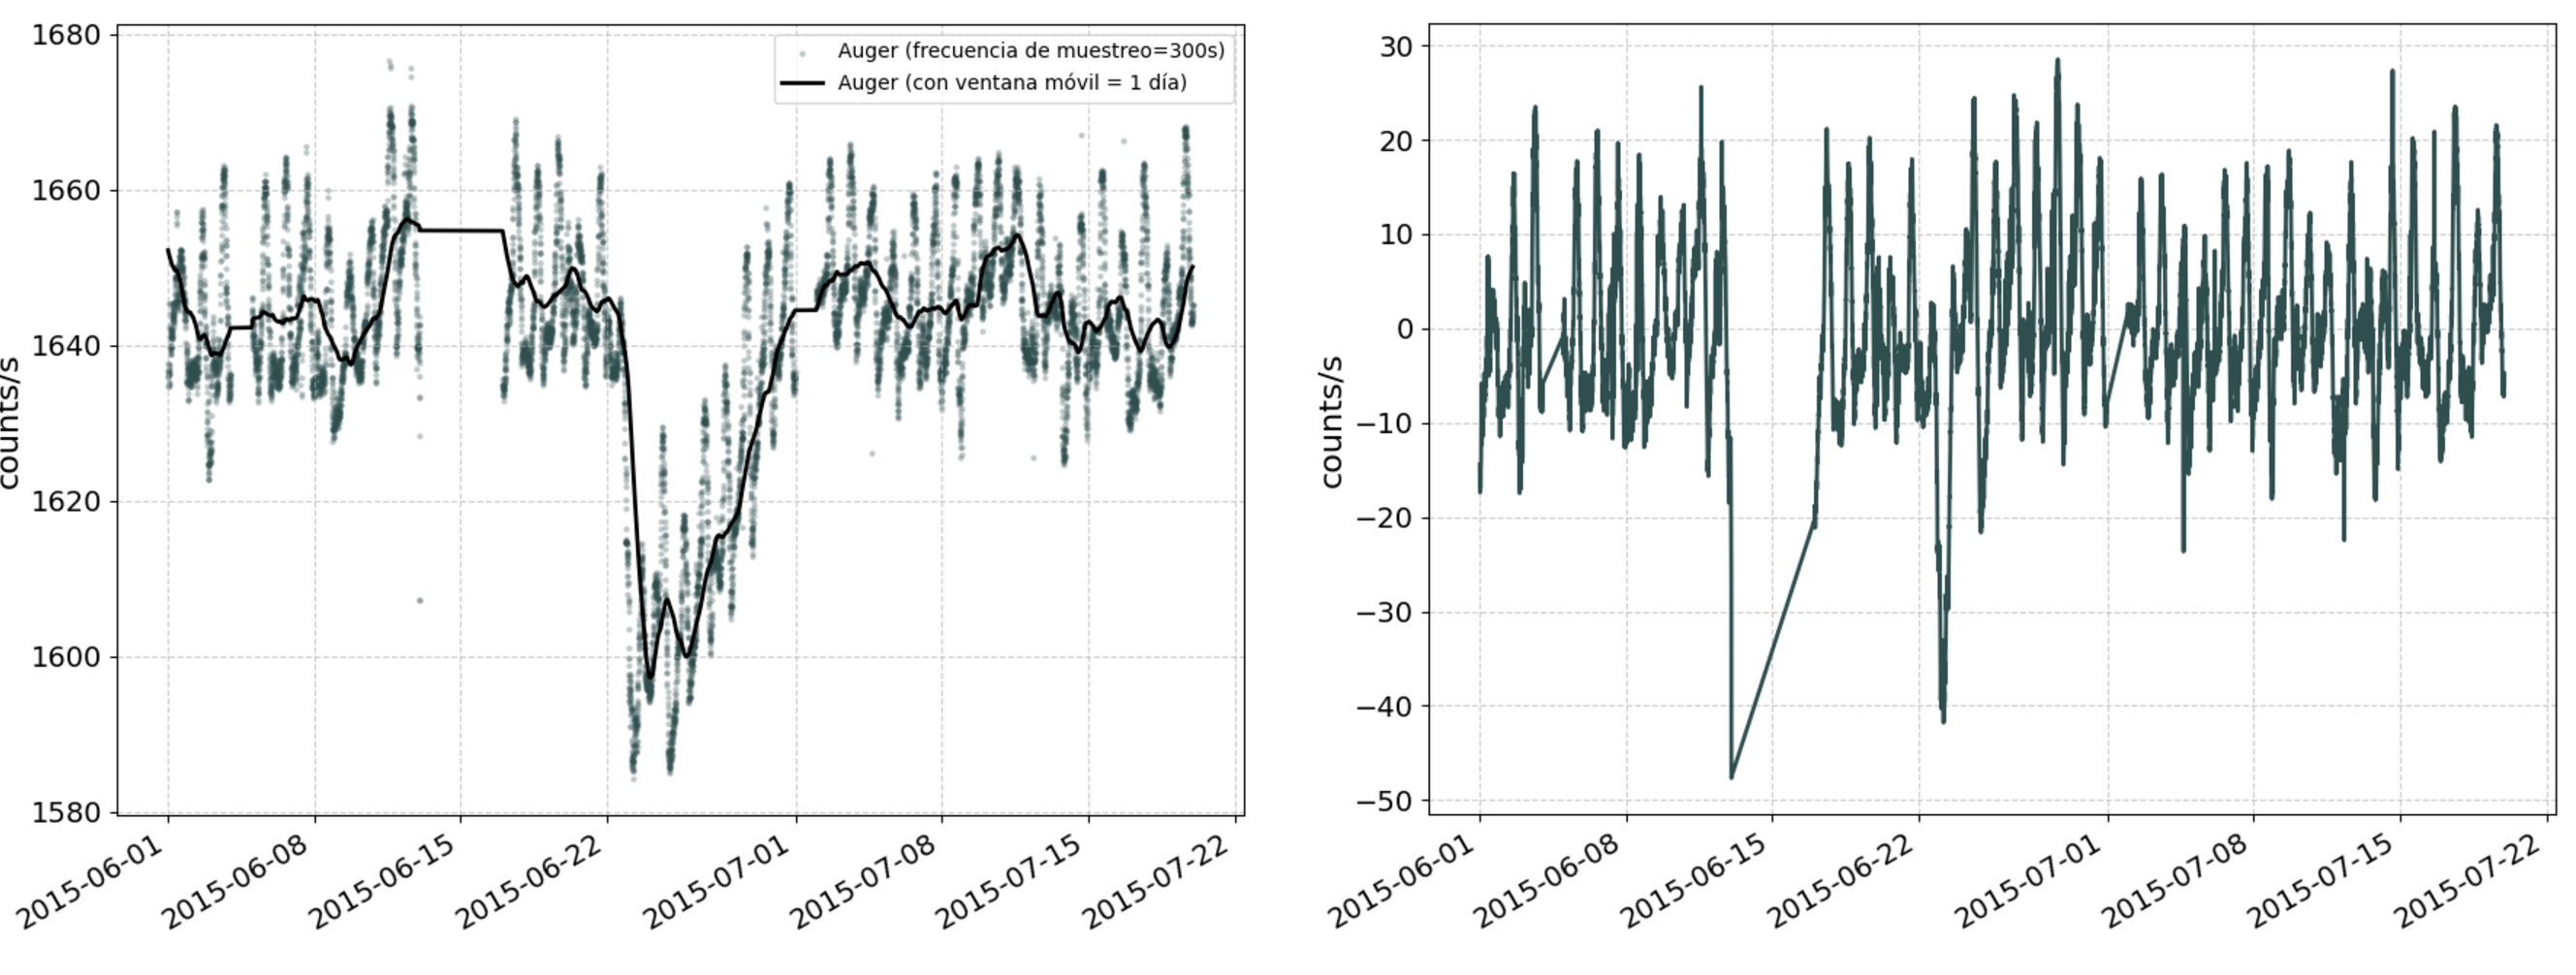
\includegraphics[width=1.1\linewidth]{Figs/Figr/forbush_filter_1D_DIFERENCIA.pdf}
    \caption{Pendiente modificar con Autocorrelación para eliminar el ruido.}
    \label{filter_result}
\end{figure}
%%%%%%%%%% O HACEMOS UNA DONDE INTENTEMOS RESTAR LOS FORBUSH 
%%%%%%%%%%% SERÍA MUCHO RETO
%%%%%%%%%%%% CALCULAR LA AMPLITUD? NO SÉ
Ahora bien, la figura \ref{filter_result} no solo muestra la comparación entre la señal original y la filtrada de este FE (izquierda)  sino también su diferencia (derecha). Con esta diferencia podemos observar la amplitud de la modulación diaria que está alrededor de las 20 cuentas/s y si a este residuo le calculamos la densidad espectral podremos ver con mayor detalle la zona de alta frecuencia de la tasa de scaler tal y como se muestra en la figura \ref{forbush_filter}

\begin{figure}
\centering
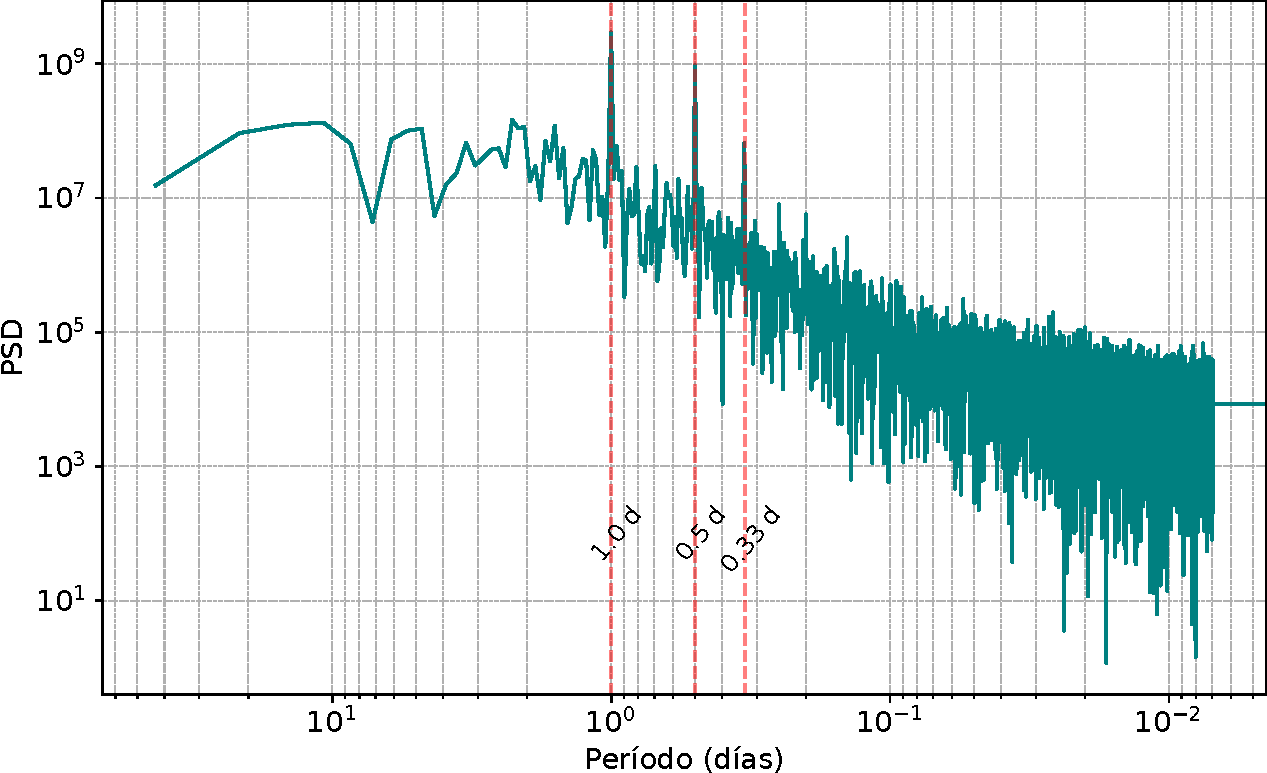
\includegraphics[width=1\linewidth]{Figs/Figr/forbush_difference_FFT.pdf}
    \caption{Pendiente modificar con Autocorrelación para eliminar el ruido.}
    \label{forbush_filter}
    \end{figure}
    En la gráfica podemos observar muy marcados la evidencia de tres armónicos principales en la señal, correspondientes a 24, 12 y 8h, la modulación de 24 horas como se mencionó en la sección anterior, está relacionada con la rotación de la Tierra. La modulación a 12 horas es llamada \textit{modulación semidiurna} (\cite{nicolson_1948}, \cite{grieder_2001}) también asociada a la interacción del campo geomagnético con el viento solar (\cite{singh_2015}, \cite{sarabhai_1953}) además se observan dos armónicos menos prominentes cerca a 4,8 y 6h que han sido también observados en  detectores de neutrones (\cite{shalaby_2022}). Los mecanismos de transporte que originan estas fluctuaciones siguen siendo un problema de estudio en la actualidad lo que permite que el Observatorio Pierre Auger pueda contribuir  gracias a la sensibilidad a las altas frecuencias, al estudio de estos fenómenos de corto plazo.

Un análisis más detallado de esta periodicidad debe descomponer los armónicos de la señal diurna, la componente de 27 y 365 para construir el fondo para ser suprimido de la señal, para caracterizar de forma más precisa la amplitud de la variación en la CRI generada por los FE como se propone en el trabajo de O. Okike (2020). Sin embargo, es posible calcular una referencia en la amplitud de los Forbush y por ende su sensibilidad, a partir de la señal filtrada que tenemos y la aplicación del método manual, usado predominantemente en los estudios de FE (\cite{okike_2020}). 

El método manual ha consistido en inspeccionar visualmente los datos de CRI, trazar ciertos segmentos y determinar la magnitud del evento como se describe a continuación: primero se comienza seleccionando un subconjunto de los datos CRI brutos para su trazado. Como referencia usaremos el FE del 22 de junio del 2015 anteriormente descrito e ilustrado en el panel derecho de la figura \ref{filter_result}. Por inspección se identifican las cuatro fases esenciales de un evento Forbush -inicio, fase principal, punto mínimo y fase de recuperación-. Un evento de Disminución de Forbush (FD) como se explicó en el capítulo 1, se caracteriza generalmente por una disminución que dura uno o más días, alcanzando un mínimo seguido de una recuperación gradual. En este proceso de identificación, el evento proyectado se descarta si falta alguna de estas fases. 

La etapa siguiente, que es la determinación de la magnitud del evento FD. Para ello, hay que normalizar los datos, determinar el tamaño del evento, seleccionar el inicio del evento y el punto mínimo de reducción de intensidad. Dependiendo de la línea de base utilizada, el proceso de normalización puede abordarse por ejemplo utilizando la variación media de CR durante el periodo o el recuento previo al día del mínimo del FE, de tal manera que la magnitud queda determinada como:
\begin{equation}
    FD_{amplitude}(\%)=\frac{FD_{inicio}-mean}{mean} *100
\end{equation}
Cabe resaltar que aunque este método sigue siendo pertinente, recientemente se ha propuesto un método automatizado para hacer la identificación de Forbush (\cite{okike_2020}) que puede ser implementado en los datos del Observatorio Pierre Auger si se realiza una correcta catacterización del fondo a través de un análisis espectral mucho más detallado. En concordancia al análisis manual descrito, la figura \ref{22junio2015} muestra el resultado de la identificación de la amplitud de nuestro FD seleccionado que para nuestra señal filtrada es de $3.01\%$ en contraste a los reportes de las estaciones de neutrones que registraron un doble FD importante con una amplitud del $8,4\%$ y del $ 5,2\%$ en las estaciones polares (\cite{samara_2018}), o de las estimaciones realizadas a partir de datos satelitales del AMS que llega a valores de $15.2\%$ (\cite{wang_2023}), lo que confirma la necesidad de remover las otras componentes periódicas de la señal.
\begin{figure}
\centering
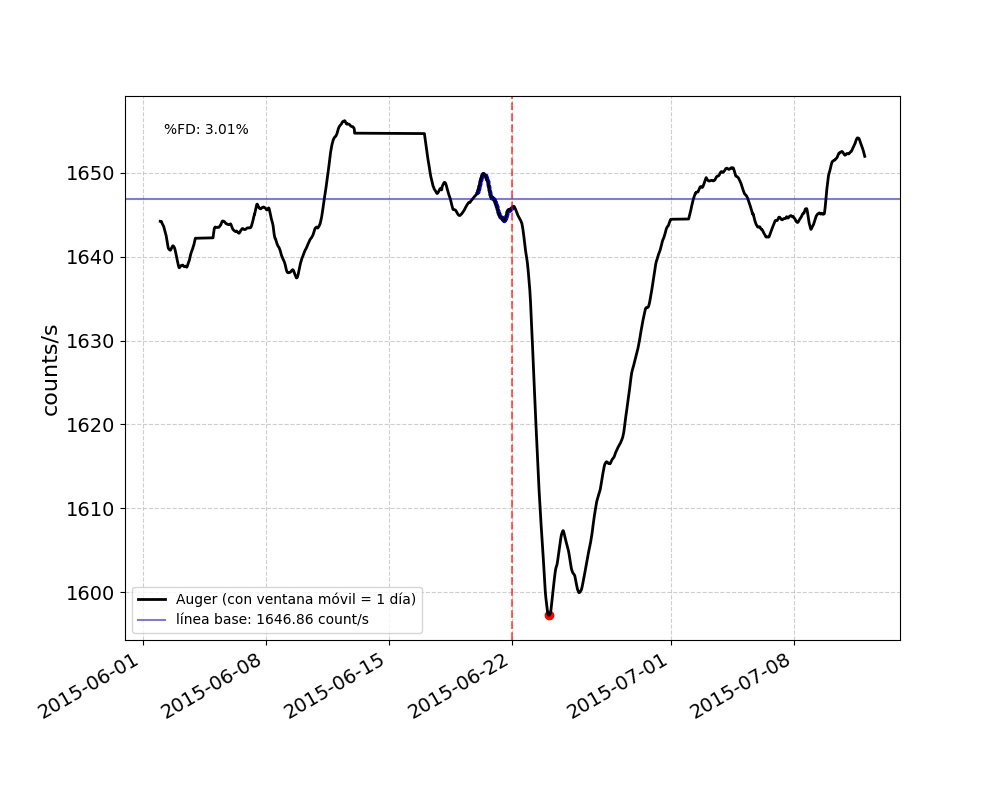
\includegraphics[width=1\linewidth]{Figs/Figr/2015-06-22 00:00:00.png}
    \caption{Pendiente modificar con Autocorrelación para eliminar el ruido.}
    \label{22junio2015}
    \end{figure}

\section{Datos abiertos y ciencia ciudadana}
\newpage
\chapter{Conclusiones}

Se realizó un análisis de la intensidad de rayos cósmicos CRI medido en el Observatorio Pierre Auger a través de las mediciones en modo \textit{scaler}. Para tal fin se tuvieron en cuenta los registros  que corresponden al periodo 2006-2021, cubriendo todo el ciclo solar 24.  Usando diferentes métodos para el análisis de series de tiempo, se observó que los \textit{scaler} tienen una respuesta a la modulación de la actividad solar a largo plazo sobre el flujo de GCR en concordancia a su rigidez de corte geomagnético $R_C=9,8 GV$ en comparación con otros detectores de neutrones ubicados a diferentes latitudes alrededor del mundo. 

La correlación entre la intensidad de rayos cósmicos y el histórico de número de manchas solares es moderada (entre  0.30 y 0.50) como se observó en la (figura \ref{fig:sunspots_corr}). Este resultado se encuentra en el mismo rango que el obtenido para la estación de Tsumeb que tiene una rigidez de corte de $R_C=9.15 GV$. Esta simulitud sugiere que el resultado puede estar relacionado a la rigidez de corte geomagnético que disminuye la sensibilidad considerablemente. Para el análisis de correlación, también se usó como valor de referencia la estación de Oulu cuyos datos han sido ampliamente estudiados por la comunidad científica debido a su rigidez de corte $R_C=0.81 GV$ , accesibilidad y consistencia en las mediciones a lo largo del tiempo. Para esta estación se observa una correlación fuerte mayor al 0.5  para el número de manchas solares.  Por otro lado, se observó una correlación débil (entre 0.10 y 0.29) con el viento solar esto se mantuvo también para las dos estaciones de neutrones consideradas en este estudio. La baja anticorrelación observada entre la intensidad de los rayos cósmicos y la velocidad del viento solar puede atribuirse a las propiedades del viento solar, específicamente el viento solar rápido, que se origina en los agujeros coronales del Sol y es notablemente estable (\cite{Oloketuyi_2020}).
%Especialmente hemos replicado los análisis de correlación efectuados en el trabajo de Oloketuyi y colaboradores \cite{Oloketuyi_2020}. 

También se realizó un análisis espectral a través de la transformada de Fourier y la función de autocorrelación que arroja una componente diaria, mensual y anual (figura\ref{FFT1}). Estas modulaciones han sido identificadas y analizadas previamente en la estaciones de neutrones y están relacionadas con la forma como el campo magnético de la Tierra interactúa con la heliósfera y sus perturbaciones asociadas la rotación solar. 

De la misma forma, se hizo un análisis cualitativo de la sensibilidad que tiene el observatorio a modulaciones a corto plazo, para identificar posibles efectos en la tasa de incidencia de eventos transitorios y la modulación en el ciclo solar. Para esto se utilizó el catálogo de eventos Forbush y disturbios interplanetarios del IZMIRAN (El Instituto Pushkov de Magnetismo Terrestre, Ionosfera y Propagación de Ondas de Radio de la Academia Rusa de Ciencias). De allí se seleccionaron aquellos eventos que estuvieran asociados a ondas de choque interplanetarias OCI o a una tormenta geomagnética de inicio repentino SSC (eventos asociados a ICME) (ver figura \ref{fig:FD_events}). Como resultado, se identificó una muestra de 148 eventos entre el 2006 y 2021 (con un nivel confianza razonable). Se observó que la mayor incidencia de FD $55.41\%$  ocurre en la zona de máxima actividad solar, específicamente en la zona de mayor anomalía en elcomportamiento de los Scaler medidos. En esta región también se encuentra el $71.20\%$ de los eventos con magnitud $>= 2\%$ respecto a todo el periodo de registro del Observatorio.

Ahora, disminuyendo cada vez más la ventana de observación de la señal, se realizó un filtrado de la modulación diaria sobre los datos de scaler y se seleccionó para su análisis el FE del 22 de junio del 2015 reportado en la base de datos con una magnitud del $9.6\%$ generada por dos llamaradas solares que corresponden al segundo evento más intenso del ciclo solar 24 y el mayor del que se tienen datos de scaler disponibles en el Observatorio Pierre Auger (figura \ref{22junio2015}). A partir de la señal original y la señal filtrada se obtuvo la densidad espectral de potencia que permitió ver con mayor nivel de detalle la zona de más alta frecuencia. Se observó evidencia de modulaciones a 24, 12, 8, 6 y 4.8 horas, reportadas también en algunos detectores de neutrones. La evidencia de la señal observada a 8 horas tiene muy pocos registros en la literatura y debe ser estudiada con mayor nivel de detalle. En general la explicación de las interacciones geomagnéticas detrás de estas modulaciones en la intensidad de rayos cósmicos, sigue siendo un problema abierto en este campo de estudio. 

Finalmente, se calculó la magnitud del FD obteniendo un porcentaje de decrecimiento del $3.01\%$ que es un valor muy por debajo de los que se reportan en la literatura (entre $5.2\%$ y el $15.2\%$) lo que sugiere que para determinar la capacidad de resolución de FD no recurrentes, se debe hacer una caracterización más robusta del fondo.   % Conclusiones
% ------------------------------------------------------------------------
% Bibliografía
% ------------------------------------------------------------------------
\addcontentsline{toc}{chapter}{Referencias Bibliográficas}\newpage %%% JENN REMOVIDO
%\noindent
%\bibliographystyle{apalike}
\printbibliography %%% JENN REMOVIDO
% ------------------------------------------------------------------------
% Anexos
% ------------------------------------------------------------------------
\newpage
%%%%%%%%%%%%%%%%%%%%%%%%%%%%----->SECCIÓN 2<-----%%%%%%%%%%%%%%%%%%%%%%%%%
\chapter{Anexos}
%%%%%%%%%%%%%%%%%% NEWWWW

%%%%% INSERTE TABLA BEBÉ
\begin{longtable}{lllllllll}
\caption{Caption} \\
\toprule
\textbf{Date} & \textbf{Sdate} & \textbf{Stime} & \textbf{Stype} & \textbf{Qs} & \textbf{MagnM} & \textbf{Dstmin} & \textbf{SSN} & \textbf{Vmax} \\ 
\midrule
\endhead
% contenido de la tabla
2006-07-09 21:36:00 & 2006-07-06 & 8:13:00 & 1.0 & 4.0 & 3.8 & -23.0 & 31.0 & 438.0 \\ 
        2006-07-27 13:53:00 & ~ & ~ & 8.0 & 4.0 & 1.0 & -47.0 & 18.0 & 663.0 \\ 
        2006-08-07 00:35:00 & ~ & ~ & 8.0 & 4.0 & 0.9 & -44.0 & 0.0 & 630.0 \\ 
        2006-12-08 04:35:00 & 2006-12-06 & 18:29:00 & 1.0 & 4.0 & 1.8 & -29.0 & 28.0 & 702.0 \\ 
        2006-12-14 14:14:00 & 2006-12-13 & 2:14:00 & 1.0 & 5.0 & 9.6 & -146.0 & 23.0 & 955.0 \\ 
        2006-12-16 17:55:00 & 2006-12-14 & 21:07:00 & 1.0 & 4.0 & 0.8 & -43.0 & 20.0 & 779.0 \\ 
        2006-12-18 10:14:00 & ~ & ~ & 6.0 & 4.0 & 0.9 & -34.0 & 0.0 & 736.0 \\ 
        2007-05-07 08:26:00 & 2007-05-02 & 18:05:00 & 6.0 & 4.0 & 1.1 & -31.0 & 13.0 & 638.0 \\ 
        2007-09-20 10:12:00 & ~ & ~ & 8.0 & 4.0 & 1.4 & -13.0 & 0.0 & 674.0 \\ 
        2007-10-25 11:35:00 & ~ & ~ & 8.0 & 4.0 & 0.9 & -52.0 & 0.0 & 698.0 \\ 
        2007-12-17 02:53:00 & ~ & ~ & 8.0 & 4.0 & 1.2 & -38.0 & 19.0 & 697.0 \\ 
        2008-01-31 11:23:00 & ~ & ~ & 8.0 & 4.0 & 0.6 & -30.0 & 10.0 & 461.0 \\ 
        2008-04-30 15:57:00 & 2008-04-26 & 13:54:00 & 6.0 & 4.0 & 1.0 & -23.0 & 0.0 & 518.0 \\ 
        2008-05-28 02:25:00 & ~ & ~ & 8.0 & 4.0 & 1.1 & -21.0 & 0.0 & 538.0 \\ 
        2008-09-30 12:34:00 & ~ & ~ & 8.0 & 4.0 & 1.0 & -27.0 & 0.0 & 715.0 \\ 
        2008-11-15 16:25:00 & ~ & ~ & 8.0 & 4.0 & 0.7 & -29.0 & 13.0 & 525.0 \\ 
        2008-11-24 23:51:00 & ~ & ~ & 8.0 & 4.0 & 1.2 & -12.0 & 0.0 & 658.0 \\ 
        2008-12-16 11:59:00 & ~ & ~ & 2.0 & 4.0 & 1.4 & -15.0 & 0.0 & 370.0 \\ 
        2009-03-03 06:02:00 & ~ & ~ & 6.0 & 4.0 & 0.4 & -14.0 & 0.0 & 390.0 \\ 
        2009-04-24 00:53:00 & ~ & ~ & 8.0 & 4.0 & 0.7 & -9.0 & 0.0 & 432.0 \\ 
        2009-05-28 05:19:00 & ~ & ~ & 8.0 & 4.0 & 0.9 & -17.0 & 0.0 & 440.0 \\ 
        2009-06-20 04:51:00 & ~ & ~ & 2.0 & 4.0 & 0.5 & -3.0 & 0.0 & 353.0 \\ 
        2009-08-07 15:55:00 & ~ & ~ & 4.0 & 4.0 & 0.7 & -21.0 & 0.0 & 517.0 \\ 
        2009-09-03 15:52:00 & ~ & ~ & 8.0 & 4.0 & 0.7 & -9.0 & 0.0 & 492.0 \\ 
        2009-10-04 04:12:00 & ~ & ~ & 8.0 & 4.0 & 0.8 & -5.0 & 0.0 & 416.0 \\ 
        2009-12-05 06:51:00 & ~ & ~ & 8.0 & 4.0 & 0.9 & -11.0 & 0.0 & 420.0 \\ 
        2010-04-05 08:26:00 & 2010-04-03 & 9:04:00 & 1.0 & 4.0 & 3.1 & -76.0 & 34.0 & 814.0 \\ 
        2010-04-11 13:04:00 & 2010-04-08 & 2:30:00 & 1.5 & 4.0 & 1.6 & -67.0 & 10.0 & 457.0 \\ 
        2010-05-28 02:57:00 & 2010-05-24 & 13:05:00 & 2.0 & 4.0 & 2.7 & -80.0 & 13.0 & 385.0 \\ 
        2010-08-03 17:41:00 & 2010-08-01 & 7:55:00 & 1.0 & 4.0 & 3.7 & -74.0 & 14.0 & 598.0 \\ 
        2010-08-04 10:19:00 & ~ & ~ & 2.0 & 4.0 & 0.6 & -74.0 & 32.0 & 598.0 \\ 
        2010-10-30 10:13:00 & ~ & ~ & 2.0 & 4.0 & 1.9 & -14.0 & 33.0 & 387.0 \\ 
        2010-11-10 17:43:00 & ~ & ~ & 7.0 & 4.0 & 1.4 & -39.0 & 48.0 & 546.0 \\ 
        2011-02-14 15:55:00 & ~ & ~ & 5.0 & 4.0 & 1.3 & -40.0 & 87.0 & 497.0 \\ 
        2011-02-18 01:30:00 & 2011-02-15 & 1:44:00 & 1.0 & 4.0 & 4.7 & -30.0 & 85.0 & 691.0 \\ 
        2011-03-10 06:45:00 & 2011-03-07 & 19:43:00 & 1.0 & 4.0 & 3.0 & -83.0 & 83.0 & 405.0 \\ 
        2011-03-29 16:30:00 & 2011-03-24 & 12:01:00 & 2.0 & 4.0 & 2.9 & -4.0 & 104.0 & 391.0 \\ 
        2011-04-01 16:48:00 & ~ & ~ & 6.0 & 4.0 & 2.2 & -38.0 & 67.0 & 650.0 \\ 
        2011-04-06 09:33:00 & ~ & ~ & 2.0 & 4.0 & 1.5 & -60.0 & ~ & 539.0 \\ 
        2011-06-04 20:44:00 & 2011-06-02 & 7:22:00 & 1.0 & 4.0 & 3.4 & -45.0 & 115.0 & 556.0 \\ 
        2011-08-05 17:51:00 & 2011-08-04 & 3:41:00 & 1.0 & 4.0 & 4.8 & -115.0 & 88.0 & 611.0 \\ 
        2011-09-09 12:42:00 & 2011-09-06 & 1:35:00 & 1.0 & 4.0 & 3.2 & -75.0 & 72.0 & 560.0 \\ 
        2011-09-25 11:45:00 & 2011-09-22 & 10:29:00 & 1.0 & 4.0 & 1.3 & -7.0 & 122.0 & 367.0 \\ 
        2011-09-26 12:35:00 & 2011-09-24 & 12:33:00 & 1.0 & 4.0 & 5.1 & -118.0 & 112.0 & 704.0 \\ 
        2011-11-12 05:59:00 & 2011-11-09 & 13:04:00 & 1.0 & 5.0 & 0.8 & -13.0 & 157.0 & 464.0 \\ 
        2012-01-22 06:11:00 & 2012-01-19 & 13:44:00 & 1.5 & 4.0 & 3.4 & -69.0 & 109.0 & 459.0 \\ 
        2012-01-24 15:03:00 & 2012-01-23 & 3:38:00 & 1.0 & 4.0 & 3.2 & -80.0 & 86.0 & 673.0 \\ 
        2012-01-30 16:24:00 & 2012-01-27 & 17:37:00 & 1.0 & 4.0 & 2.2 & -19.0 & 62.0 & 427.0 \\ 
        2012-03-07 04:20:00 & 2012-03-04 & 10:29:00 & 1.0 & 4.0 & 3.8 & -85.0 & 106.0 & 592.0 \\ 
        2012-03-08 11:03:00 & 2012-03-07 & 0:02:00 & 1.0 & 5.0 & 11.2 & -143.0 & 97.0 & 737.0 \\ 
        2012-03-11 13:00:00 & 2012-03-09 & 3:22:00 & 1.0 & 5.0 & 0.8 & -44.0 & 116.0 & 461.0 \\ 
        2012-03-12 09:14:00 & 2012-03-10 & 17:15:00 & 1.0 & 5.0 & 5.8 & -51.0 & 116.0 & 727.0 \\ 
        2012-03-15 13:06:00 & 2012-03-13 & 17:12:00 & 1.0 & 5.0 & 1.8 & -80.0 & 88.0 & 787.0 \\ 
        2012-04-23 03:20:00 & ~ & ~ & 2.0 & 4.0 & 1.7 & -103.0 & 138.0 & 394.0 \\ 
        2012-05-21 19:37:00 & ~ & ~ & 4.0 & 4.0 & 0.8 & -24.0 & 110.0 & 430.0 \\ 
        2012-06-16 09:55:00 & 2012-06-13 & 11:29:00 & 1.0 & 4.0 & 1.1 & 15.0 & 106.0 & 413.0 \\ 
        2012-06-16 20:20:00 & 2012-06-14 & 12:52:00 & 1.0 & 4.0 & 4.0 & -71.0 & 106.0 & 519.0 \\ 
        2012-07-14 18:09:00 & 2012-07-12 & 15:37:00 & 1.0 & 4.0 & 7.6 & -127.0 & 125.0 & 667.0 \\ 
        2012-07-20 04:47:00 & 2012-07-17 & 12:03:00 & 1.0 & 4.0 & 2.2 & -22.0 & 36.0 & 476.0 \\ 
        2012-07-21 16:05:00 & 2012-07-19 & 4:17:00 & 1.0 & 4.0 & 2.7 & -21.0 & 29.0 & 517.0 \\ 
        2012-09-03 12:13:00 & 2012-08-31 & 19:45:00 & 2.0 & 4.0 & 2.5 & -78.0 & 171.0 & 449.0 \\ 
        2012-09-30 11:31:00 & ~ & ~ & 2.0 & 4.0 & 1.0 & -133.0 & 99.0 & 319.0 \\ 
        2012-09-30 23:05:00 & 2012-09-27 & 23:36:00 & 1.0 & 4.0 & 2.1 & -119.0 & 99.0 & 410.0 \\ 
        2012-10-31 15:38:00 & ~ & ~ & 2.0 & 4.0 & 1.8 & -63.0 & 50.0 & 373.0 \\ 
        2012-11-12 23:11:00 & ~ & ~ & 2.0 & 4.0 & 4.1 & -108.0 & 122.0 & 454.0 \\ 
        2012-11-23 21:51:00 & ~ & ~ & 2.0 & 4.0 & 3.6 & -42.0 & 78.0 & 409.0 \\ 
        2013-01-19 17:32:00 & 2013-01-16 & 18:21:00 & 1.0 & 4.0 & 0.8 & -34.0 & 47.0 & 438.0 \\ 
        2013-02-16 12:09:00 & 2013-02-12 & 22:50:00 & 2.0 & 4.0 & 1.8 & -20.0 & 40.0 & 407.0 \\ 
        2013-03-15 05:26:00 & 2013-03-12 & 10:17:00 & 2.0 & 4.0 & 1.7 & -25.0 & 111.0 & 475.0 \\ 
        2013-03-17 05:59:00 & 2013-03-15 & 5:46:00 & 1.5 & 5.0 & 4.3 & -132.0 & 119.0 & 725.0 \\ 
        2013-04-13 22:54:00 & 2013-04-11 & 6:55:00 & 1.0 & 5.0 & 4.4 & -6.0 & 117.0 & 516.0 \\ 
        2013-04-30 09:49:00 & ~ & ~ & 4.0 & 4.0 & 2.3 & -24.0 & 150.0 & 426.0 \\ 
        2013-05-18 01:10:00 & 2013-05-15 & 1:25:00 & 1.0 & 4.0 & 2.1 & -61.0 & 133.0 & 439.0 \\ 
        2013-05-19 23:08:00 & 2013-05-17 & 8:43:00 & 1.0 & 5.0 & 0.8 & -30.0 & 127.0 & 422.0 \\ 
        2013-05-24 18:10:00 & 2013-05-22 & 13:08:00 & 1.0 & 4.0 & 1.2 & -55.0 & 108.0 & 555.0 \\ 
        2013-05-25 09:48:00 & ~ & ~ & 1.5 & 4.0 & 2.4 & -51.0 & 118.0 & 777.0 \\ 
        2013-05-31 16:18:00 & ~ & ~ & 2.0 & 4.0 & 2.2 & -124.0 & 50.0 & 684.0 \\ 
        2013-06-23 04:26:00 & 2013-06-21 & 2:30:00 & 4.0 & 4.0 & 5.3 & -49.0 & 118.0 & 697.0 \\ 
        2013-06-27 14:38:00 & ~ & ~ & 2.0 & 4.0 & 2.8 & -98.0 & 61.0 & 453.0 \\ 
        2013-07-12 17:14:00 & ~ & ~ & 2.0 & 4.0 & 2.7 & -56.0 & 73.0 & 509.0 \\ 
        2013-08-20 22:28:00 & 2013-08-17 & 18:16:00 & 1.0 & 4.0 & 0.8 & -26.0 & 129.0 & 465.0 \\ 
        2013-08-24 00:03:00 & ~ & ~ & 4.0 & 4.0 & 2.6 & -23.0 & 78.0 & 521.0 \\ 
        2013-10-02 01:55:00 & 2013-09-29 & 21:43:00 & 2.0 & 4.0 & 3.7 & -67.0 & 60.0 & 629.0 \\ 
        2013-10-08 20:23:00 & 2013-10-06 & 13:37:00 & 5.0 & 4.0 & 1.9 & -62.0 & 96.0 & 639.0 \\ 
        2013-12-13 13:22:00 & 2013-12-07 & 7:17:00 & 1.0 & 4.0 & 1.2 & -1.0 & 144.0 & 392.0 \\ 
        2014-01-07 15:12:00 & 2014-01-04 & 19:05:00 & 1.0 & 5.0 & 1.5 & -26.0 & 140.0 & 440.0 \\ 
        2014-01-09 20:08:00 & 2014-01-07 & 18:04:00 & 1.0 & 5.0 & 2.3 & -24.0 & 120.0 & 436.0 \\ 
        2014-02-13 09:44:00 & ~ & ~ & 2.0 & 4.0 & 0.7 & -1.0 & 147.0 & 381.0 \\ 
        2014-02-15 13:16:00 & 2014-02-12 & 15:41:00 & 1.0 & 4.0 & 3.6 & -27.0 & 113.0 & 450.0 \\ 
        2014-02-20 03:18:00 & 2014-02-17 & 2:51:00 & 1.0 & 4.0 & 2.8 & -86.0 & 133.0 & 691.0 \\ 
        2014-02-27 16:50:00 & 2014-02-25 & 0:39:00 & 1.0 & 5.0 & 4.9 & -99.0 & 220.0 & 483.0 \\ 
        2014-03-25 20:03:00 & 2014-03-23 & 3:05:00 & 1.0 & 4.0 & 1.5 & -22.0 & 136.0 & 516.0 \\ 
        2014-04-20 10:57:00 & 2014-04-18 & 12:31:00 & 1.0 & 4.0 & 1.5 & -24.0 & 173.0 & 678.0 \\ 
        2014-04-29 20:26:00 & ~ & ~ & 4.0 & 4.0 & 1.5 & -64.0 & 77.0 & 309.0 \\ 
        2014-05-29 09:30:00 & ~ & ~ & 7.0 & 4.0 & 0.7 & -17.0 & 48.0 & 360.0 \\ 
        2014-06-07 16:52:00 & ~ & ~ & 2.0 & 4.0 & 3.9 & -38.0 & 133.0 & 616.0 \\ 
        2014-06-23 23:08:00 & 2014-06-19 & 18:36:00 & 2.0 & 5.0 & 0.4 & -9.0 & 77.0 & 361.0 \\ 
        2014-07-03 00:42:00 & ~ & ~ & 2.0 & 4.0 & 0.4 & -21.0 & 167.0 & 347.0 \\ 
        2014-08-19 06:57:00 & ~ & ~ & 2.0 & 4.0 & 1.4 & -32.0 & 93.0 & 419.0 \\ 
        2014-09-06 15:24:00 & ~ & ~ & 2.0 & 4.0 & 1.7 & -12.0 & 142.0 & 412.0 \\ 
        2014-09-11 23:45:00 & 2014-09-08 & 23:12:00 & 1.0 & 5.0 & 2.1 & -16.0 & 160.0 & 467.0 \\ 
        2014-09-12 15:53:00 & 2014-09-10 & 17:21:00 & 1.0 & 5.0 & 5.9 & -75.0 & 126.0 & 730.0 \\ 
        2014-11-01 07:05:00 & ~ & ~ & 5.0 & 4.0 & 1.6 & -9.0 & 90.0 & 522.0 \\ 
        2014-11-10 02:20:00 & 2014-11-07 & 16:53:00 & 1.0 & 4.0 & 3.6 & -57.0 & 69.0 & 509.0 \\ 
        2014-12-21 19:11:00 & 2014-12-17 & 4:25:00 & 1.0 & 4.0 & 6.0 & -51.0 & 137.0 & 429.0 \\ 
        2014-12-22 15:10:00 & 2014-12-18 & 21:41:00 & 1.0 & 4.0 & 2.0 & -21.0 & 118.0 & 477.0 \\ 
        2014-12-23 11:14:00 & 2014-12-20 & 0:11:00 & 1.0 & 4.0 & 2.7 & -25.0 & 115.0 & 508.0 \\ 
        2015-01-07 06:14:00 & ~ & ~ & 2.0 & 4.0 & 1.2 & -99.0 & 103.0 & 485.0 \\ 
        2015-03-17 04:45:00 & 2015-03-15 & 1:15:00 & 1.0 & 4.0 & 5.6 & -223.0 & 38.0 & 609.0 \\ 
        2015-04-09 02:13:00 & 2015-04-04 & 22:16:00 & 2.0 & 4.0 & 1.9 & -7.0 & 47.0 & 385.0 \\ 
        2015-04-14 06:16:00 & ~ & ~ & 7.0 & 4.0 & 1.0 & -59.0 & 105.0 & 727.0 \\ 
        2015-05-06 01:42:00 & ~ & ~ & 2.0 & 4.0 & 2.6 & -28.0 & 124.0 & 479.0 \\ 
        2015-06-21 16:44:00 & 2015-06-18 & 16:30:00 & 1.0 & 4.0 & 0.9 & -3.0 & 61.0 & 350.0 \\ 
        2015-06-22 05:44:00 & ~ & ~ & 2.0 & 4.0 & 1.3 & -51.0 & 56.0 & 436.0 \\ 
        2015-06-22 18:33:00 & 2015-06-21 & 2:06:00 & 1.0 & 4.0 & 9.1 & -204.0 & 56.0 & 742.0 \\ 
        2015-07-10 15:54:00 & ~ & ~ & 6.0 & 4.0 & 1.7 & -28.0 & 103.0 & 637.0 \\ 
        2015-07-13 01:38:00 & ~ & ~ & 2.0 & 4.0 & 3.0 & -61.0 & 53.0 & 644.0 \\ 
        2015-07-30 15:37:00 & ~ & ~ & 8.0 & 4.0 & 1.3 & -30.0 & 76.0 & 613.0 \\ 
        2015-08-15 08:28:00 & 2015-08-12 & 14:26:00 & 2.0 & 4.0 & 2.0 & -84.0 & 39.0 & 536.0 \\ 
        2015-08-28 12:49:00 & ~ & ~ & 6.0 & 4.0 & 1.0 & -88.0 & 44.0 & 477.0 \\ 
        2015-09-20 06:03:00 & 2015-09-18 & 4:22:00 & 1.0 & 4.0 & 1.4 & -75.0 & 65.0 & 621.0 \\ 
        2015-10-24 18:54:00 & 2015-10-22 & 2:13:00 & 1.5 & 4.0 & 1.1 & -7.0 & 78.0 & 499.0 \\ 
        2015-11-03 01:34:00 & ~ & ~ & 6.0 & 4.0 & 1.3 & -55.0 & 82.0 & 713.0 \\ 
        2015-11-06 18:18:00 & 2015-11-04 & 13:31:00 & 1.0 & 4.0 & 3.1 & -96.0 & 78.0 & 677.0 \\ 
        2015-12-14 13:21:00 & 2015-12-11 & 16:48:00 & 1.0 & 4.0 & 1.7 & -47.0 & 86.0 & 544.0 \\ 
        2015-12-19 16:16:00 & 2015-12-16 & 8:34:00 & 1.0 & 4.0 & 3.1 & -71.0 & 49.0 & 497.0 \\ 
        2015-12-31 00:50:00 & 2015-12-28 & 11:20:00 & 1.0 & 4.0 & 5.2 & -110.0 & 22.0 & 485.0 \\ 
        2016-01-18 21:57:00 & ~ & ~ & 2.0 & 5.0 & 2.0 & -93.0 & 54.0 & 383.0 \\ 
        2016-03-14 17:14:00 & ~ & ~ & 7.0 & 4.0 & 1.1 & -50.0 & 70.0 & 567.0 \\ 
        2016-04-02 14:31:00 & ~ & ~ & 7.0 & 4.0 & 1.0 & -56.0 & 12.0 & 508.0 \\ 
        2016-07-19 23:51:00 & 2016-07-17 & 5:36:00 & 1.0 & 4.0 & 2.8 & -23.0 & 59.0 & 576.0 \\ 
        2016-10-12 22:12:00 & ~ & ~ & 2.0 & 4.0 & 1.8 & -104.0 & 41.0 & 440.0 \\ 
        2016-11-09 06:43:00 & ~ & ~ & 2.0 & 4.0 & 0.8 & -20.0 & 14.0 & 371.0 \\ 
        2017-01-26 08:15:00 & ~ & ~ & 6.0 & 4.0 & 0.8 & -28.0 & ~ & 636.0 \\ 
        2017-03-27 03:45:00 & ~ & ~ & 8.0 & 4.0 & 1.0 & -74.0 & ~ & 708.0 \\ 
        2017-05-27 15:34:00 & ~ & ~ & 2.0 & 4.0 & 2.9 & -125.0 & ~ & 401.0 \\ 
        2017-07-16 05:59:00 & 2017-07-14 & 1:07:00 & 1.0 & 5.0 & 5.8 & -72.0 & ~ & 625.0 \\ 
        2017-08-31 05:38:00 & 2017-08-28 & 15:33:00 & 5.0 & 4.0 & 1.0 & -50.0 & ~ & 638.0 \\ 
        2017-09-06 23:43:00 & 2017-09-04 & 20:28:00 & 1.0 & 5.0 & 1.8 & -23.0 & ~ & 581.0 \\ 
        2017-09-07 23:00:00 & 2017-09-06 & 11:53:00 & 1.0 & 5.0 & 7.7 & -124.0 & ~ & 817.0 \\ 
        2017-09-12 20:02:00 & 2017-09-10 & 15:35:00 & 1.0 & 5.0 & 1.0 & -35.0 & ~ & 621.0 \\ 
        2017-09-14 11:16:00 & ~ & ~ & 7.0 & 4.0 & 1.9 & -53.0 & ~ & 715.0 \\ 
        2017-10-21 06:10:00 & ~ & ~ & 5.0 & 4.0 & 1.1 & -14.0 & ~ & 481.0 \\ 
        2017-11-27 14:42:00 & ~ & ~ & 8.0 & 4.0 & 1.0 & -19.0 & ~ & 480.0 \\ 
        2017-12-04 16:13:00 & ~ & ~ & 8.0 & 4.0 & 1.5 & -45.0 & ~ & 622.0 \\ 
        2018-01-08 06:48:00 & ~ & ~ & 7.0 & 4.0 & 1.2 & -17.0 & ~ & 542.0 \\ 
        2018-02-15 08:35:00 & 2018-02-12 & 0:15:00 & 1.5 & 4.0 & 1.6 & -27.0 & ~ & 525.0 \\ 
        2018-03-09 18:06:00 & ~ & ~ & 2.0 & 4.0 & 0.9 & -39.0 & ~ & 453.0 \\
\bottomrule
\label{tab:my_label}
\end{longtable}
   
%\newpage
\anexo{Parámetros de los nuevos perfiles atmosféricos construidos con GDAS.}\label{sec:apendiceB}

%%%%%%%%%%%%%%%%%    TABLA 1 %%%%%%%%%%%%%%%%%%%%%%%%%%
\begin{table}[htb!]
\centering
\begin{minipage}{1\textwidth}
			\caption[Parámetros atmosféricos Enero.]{ \raggedright Parámetros atmosféricos para el mes de Enero.}
			\label{tab:tabla4}
			\begin{center}
				%	%	%	%	Acá va la tabla como tal
\begin{tabular}{llll}
\hline
\multicolumn{1}{c}{\textbf{Distancia [km]}} & \multicolumn{3}{c}{\textbf{Parámetros atmosféricos A,B,C}} \\ \hline
0 & -183.43 & 1237 & 1.07488e+06 \\ \hline
3.76290 & -84.5939 & 1146.93 & 952969 \\ \hline
9.70995 & -4.26996 & 1181.31 & 768112 \\ \hline
26.3624 & 0.000546666 & 1629.39 & 682201 \\ \hline
100 & 0.0112829 & 1 & 1e+09 \\ \hline
\end{tabular}
\end{center} 
		\end{minipage}
\end{table}

%%%%%%%%%%%%%%%%%    TABLA 2 %%%%%%%%%%%%%%%%%%%%%%%%%%
\begin{table}[htb!]
\centering
 \begin{minipage}{1\textwidth}
			\caption[Parámetros atmosféricos Febrero.]{ \raggedright Parámetros atmosféricos para el mes de Febrero.}
			\label{tab:tabla5}
			\begin{center}
				%	%	%	%	Acá va la tabla como tal
\begin{tabular}{llll}
\hline
\multicolumn{1}{c}{\textbf{Distancia [km]}} & \multicolumn{3}{c}{\textbf{Parámetros atmosféricos A,B,C}} \\ \hline
0 & -185.777 & 1240.57 & 1.07873e+06 \\ \hline
3.76290 & -80.0252 & 1144.24 & 948226 \\ \hline
9.70995 & -4.51389 & 1176.73 & 773697 \\ \hline
26.3624 & 0.000506149 & 1628.68 & 684995 \\ \hline
100 & 0.0112829 & 1 & 1e+09 \\ \hline
\end{tabular}
\end{center} 
		\end{minipage}
\end{table}

%%%%%%%%%%%%%%%%%    TABLA 3 %%%%%%%%%%%%%%%%%%%%%%%%%%
\begin{table}[htb!]
\centering
 \begin{minipage}{1\textwidth}
			\caption[Parámetros atmosféricos Marzo.]{ \raggedright Parámetros atmosféricos para el mes de Marzo.}
			\label{tab:tabla6}
			\begin{center}
				%	%	%	%	Acá va la tabla como tal
\begin{tabular}{llll}
\hline
\multicolumn{1}{c}{\textbf{Distancia [km]}} & \multicolumn{3}{c}{\textbf{Parámetros atmosféricos A,B,C}} \\ \hline
0 & -186.091 & 1240.02 & 1.08192e+06 \\ \hline
3.76290 & -82.1356 & 1145.26 & 953386 \\ \hline
9.70995 & -4.49877 & 1177.97 & 773998 \\ \hline
26.3624 & 0.000502607 & 1634.37 & 684999 \\ \hline
100 & 0.0112829 & 1 & 1e+09 \\ \hline
\end{tabular}
\end{center}
		\end{minipage}
\end{table}

%%%%%%%%%%%%%%%%%    TABLA 4 %%%%%%%%%%%%%%%%%%%%%%%%%%
\begin{table}[htb!]
\centering
\begin{minipage}{1\textwidth}
			\caption[Parámetros atmosféricos Abril.]{ \raggedright Parámetros atmosféricos para el mes de Abril.}
			\label{tab:tabla7}
			\begin{center}
				%	%	%	%	Acá va la tabla como tal
\begin{tabular}{llll}
\hline
\multicolumn{1}{c}{\textbf{Distancia [km]}} & \multicolumn{3}{c}{\textbf{Parámetros atmosféricos A,B,C}} \\ \hline
0 & -182.28 & 1237.95 & 1.07445e+06 \\ \hline
3.76290 & -81.2229 & 1145.98 & 949767 \\ \hline
9.70995 & -4.41518 & 1179.3 & 772360 \\ \hline
26.3624 & 0.000530822 & 1641.29 & 683270 \\ \hline
100 & 0.0112829 & 1 & 1e+09 \\ \hline
\end{tabular}
\end{center} 
		\end{minipage}
\end{table}

%%%%%%%%%%%%%%%%%    TABLA 5 %%%%%%%%%%%%%%%%%%%%%%%%%%

\begin{table}[htb!]
\centering
\begin{minipage}{1\textwidth}
			\caption[Parámetros atmosféricos Mayo.]{ \raggedright Parámetros atmosféricos para el mes de Mayo.}
			\label{tab:tabla8}
			\begin{center}
				%	%	%	%	Acá va la tabla como tal
\begin{tabular}{llll}
\hline
\multicolumn{1}{c}{\textbf{Distancia [km]}} & \multicolumn{3}{c}{\textbf{Parámetros atmosféricos A,B,C}} \\ \hline
0 & -181.218 & 1236.72 & 1.07487e+06 \\ \hline
3.76290 & -81.8311 & 1146.27 & 952054 \\ \hline
9.70995 & -4.39951 & 1179.72 & 773038 \\ \hline
26.3624 & 0.00052024 & 1646.42 & 683695 \\ \hline
100 & 0.0112829 & 1 & 1e+09 \\ \hline
\end{tabular}
\end{center}
		\end{minipage}
\end{table}

%%%%%%%%%%%%%%%%%    TABLA 6 %%%%%%%%%%%%%%%%%%%%%%%%%%

\begin{table}[htb!]
\centering
 
\begin{minipage}{1\textwidth}
			\caption[Parámetros atmosféricos Junio.]{ \raggedright Parámetros atmosféricos para el mes de Junio.}
			\label{tab:tabla9}
			\begin{center}
				%	%	%	%	Acá va la tabla como tal

\begin{tabular}{llll}
\hline
\multicolumn{1}{c}{\textbf{Distancia [km]}} & \multicolumn{3}{c}{\textbf{Parámetros atmosféricos A,B,C}} \\ \hline
0 & -179.889 & 1234.4 & 1.07286e+06 \\ \hline
3.76290 & -86.019 & 1148.91 & 956774 \\ \hline
9.70995 & -3.92019 & 1184.53 & 767604 \\ \hline
26.3624 & 0.00049459 & 1607.05 & 686431 \\ \hline
100 & 0.0112829 & 1 & 1e+09 \\ \hline
\end{tabular}

\end{center} %\vspace{0.1em}
		%	{\normalsize \textbf{Fuente}: \citep[][]{Meteo1} }
		\end{minipage}
\end{table}


%%%%%%%%%%%%%%%%%    TABLA 7 %%%%%%%%%%%%%%%%%%%%%%%%%%

\begin{table}[htb!]
\centering
 
\begin{minipage}{1\textwidth}
			\caption[Parámetros atmosféricos Julio.]{ \raggedright Parámetros atmosféricos para el mes de Julio.}
			\label{tab:tabla10}
			\begin{center}
				%	%	%	%	Acá va la tabla como tal

\begin{tabular}{llll}
\hline
\multicolumn{1}{c}{\textbf{Distancia [km]}} & \multicolumn{3}{c}{\textbf{Parámetros atmosféricos A,B,C}} \\ \hline
0 & -182.313 & 1236.06 & 1.07453e+06 \\ \hline
3.76290 & -86.4462 & 1148.72 & 956044 \\ \hline
9.70995 & -3.95886 & 1184.72 & 766086 \\ \hline
26.3624 & 0.000538009 & 1622.1 & 683272 \\ \hline
100 & 0.0112829 & 1 & 1e+09 \\ \hline
\end{tabular}

\end{center} %\vspace{0.1em}
		%	{\normalsize \textbf{Fuente}: \citep[][]{Meteo1} }
		\end{minipage}
\end{table}


%%%%%%%%%%%%%%%%%    TABLA 8 %%%%%%%%%%%%%%%%%%%%%%%%%%

\begin{table}[htb!]
\centering
 
\begin{minipage}{1\textwidth}
			\caption[Parámetros atmosféricos Agosto.]{ \raggedright Parámetros atmosféricos para el mes de Agosto.}
			\label{tab:tabla11}
			\begin{center}
				%	%	%	%	Acá va la tabla como tal

\begin{tabular}{llll}
\hline
\multicolumn{1}{c}{\textbf{Distancia [km]}} & \multicolumn{3}{c}{\textbf{Parámetros atmosféricos A,B,C}} \\ \hline
0 & -186.139 & 1239.66 & 1.0789e+06 \\ \hline
3.76290 & -88.2091 & 1150.4 & 957878 \\ \hline
9.70995 & -3.68067 & 1187.35 & 763621 \\ \hline
26.3624 & 0.000518244 & 1592.17 & 685882 \\ \hline
100 & 0.0112829 & 1 & 1e+09 \\ \hline
\end{tabular}

\end{center} %\vspace{0.1em}
		%	{\normalsize \textbf{Fuente}: \citep[][]{Meteo1} }
		\end{minipage}
\end{table}

%%%%%%%%%%%%%%%%%    TABLA 9 %%%%%%%%%%%%%%%%%%%%%%%%%%

\begin{table}[htb!]
\centering
 
\begin{minipage}{1\textwidth}
			\caption[Parámetros atmosféricos Septiembre.]{ \raggedright Parámetros atmosféricos para el mes de Septiembre.}
			\label{tab:tabla12}
			\begin{center}
				%	%	%	%	Acá va la tabla como tal

\begin{tabular}{llll}
\hline
\multicolumn{1}{c}{\textbf{Distancia [km]}} & \multicolumn{3}{c}{\textbf{Parámetros atmosféricos A,B,C}} \\ \hline
0 & -183.954 & 1236.97 & 1.07739e+06 \\ \hline
3.76290 & -84.3842 & 1146.24 & 954335 \\ \hline
9.70995 & -4.15752 & 1180.68 & 769259 \\ \hline
26.3624 & 0.000540041 & 1635.2 & 682826 \\ \hline
100 & 0.0112829 & 1 & 1e+09 \\ \hline
\end{tabular}

\end{center} %\vspace{0.1em}
		%	{\normalsize \textbf{Fuente}: \citep[][]{Meteo1} }
		\end{minipage}
\end{table}


%%%%%%%%%%%%%%%%%    TABLA 10 %%%%%%%%%%%%%%%%%%%%%%%%%%

\begin{table}[htb!]
\centering
 
\begin{minipage}{1\textwidth}
			\caption[Parámetros atmosféricos Octubre.]{ \raggedright Parámetros atmosféricos para el mes de Octubre.}
			\label{tab:tabla13}
			\begin{center}
				%	%	%	%	Acá va la tabla como tal

\begin{tabular}{llll}
\hline
\multicolumn{1}{c}{\textbf{Distancia [km]}} & \multicolumn{3}{c}{\textbf{Parámetros atmosféricos A,B,C}} \\ \hline
0 & -180.852 & 1235.63 & 1.0738e+06 \\ \hline
3.76290 & -80.3508 & 1144.14 & 949685 \\ \hline
9.70995 & -4.38572 & 1176.83 & 773922 \\ \hline
26.3624 & 0.000499663 & 1644.66 & 684513 \\ \hline
100 & 0.0112829 & 1 & 1e+09 \\ \hline
\end{tabular}

\end{center} %\vspace{0.1em}
		%	{\normalsize \textbf{Fuente}: \citep[][]{Meteo1} }
		\end{minipage}
\end{table}

%%%%%%%%%%%%%%%%%    TABLA 11 %%%%%%%%%%%%%%%%%%%%%%%%%%

\begin{table}[htb!]
\centering
 
\begin{minipage}{1\textwidth}
			\caption[Parámetros atmosféricos Noviembre.]{ \raggedright Parámetros atmosféricos para el mes de Noviembre.}
			\label{tab:tabla14}
			\begin{center}
				%	%	%	%	Acá va la tabla como tal

\begin{tabular}{llll}
\hline
\multicolumn{1}{c}{\textbf{Distancia [km]}} & \multicolumn{3}{c}{\textbf{Parámetros atmosféricos A,B,C}} \\ \hline
0 & -179.222 & 1233.73 & 1.07416e+06 \\ \hline
3.76290 & -78.7574 & 1142.26 & 949893 \\ \hline
9.70995 & -4.54605 & 1173.72 & 777710 \\ \hline
26.3624 & 0.000480868 & 1639.56 & 686566 \\ \hline
100 & 0.0112829 & 1 & 1e+09 \\ \hline
\end{tabular}

\end{center} %\vspace{0.1em}
		%	{\normalsize \textbf{Fuente}: \citep[][]{Meteo1} }
		\end{minipage}
\end{table}


%%%%%%%%%%%%%%%%%    TABLA 12 %%%%%%%%%%%%%%%%%%%%%%%%%%

\begin{table}[htb!]
\centering
 
\begin{minipage}{1\textwidth}
			\caption[Parámetros atmosféricos Diciembre.]{ \raggedright Parámetros atmosféricos para el mes de Diciembre.}
			\label{tab:tabla15}
			\begin{center}
				%	%	%	%	Acá va la tabla como tal

\begin{tabular}{llll}
\hline
\multicolumn{1}{c}{\textbf{Distancia [km]}} & \multicolumn{3}{c}{\textbf{Parámetros atmosféricos A,B,C}} \\ \hline
0 & -179.336 & 1233.49 & 1.07174e+06 \\ \hline
3.76290 & -79.8575 & 1142.9 & 948863 \\ \hline
9.70995 & -4.93372 & 1174.98 & 775317 \\ \hline
26.3624 & 0.000593498 & 1695.48 & 677150 \\ \hline
100 & 0.0112829 & 1 & 1e+09 \\ \hline
\end{tabular}

\end{center} %\vspace{0.1em}
		%	{\normalsize \textbf{Fuente}: \citep[][]{Meteo1} }
		\end{minipage}
\end{table}

\clearpage
\newpage
\newpage




   
%\newpage
\newpage
\anexo{Distribuciones longitudinales de primarios individuales}\label{sec:apendiceC}


Las siguientes gráficas corresponden, cada uno, a distribuciones longitudinales de primarios individuales, usando la atmósfera predeterminada (línea azul), y usando la atmósfera construida para el mes de abril (línea roja). Se observa el número de partículas que se genera, a medida que la EAS se desarrolla a través de la atmósfera (superior izquierda), la diferencia porcentual en relación al número de partículas generadas con la atmósfera predeterminada (inferior izquierda), la energía depositada a lo largo del desarrollo de la EAS (superior derecha), y la diferencia porcentual en relación a la energía depositada con la atmósfera predeterminada (inferior derecha).

\begin{figure}[htb!]
\centering
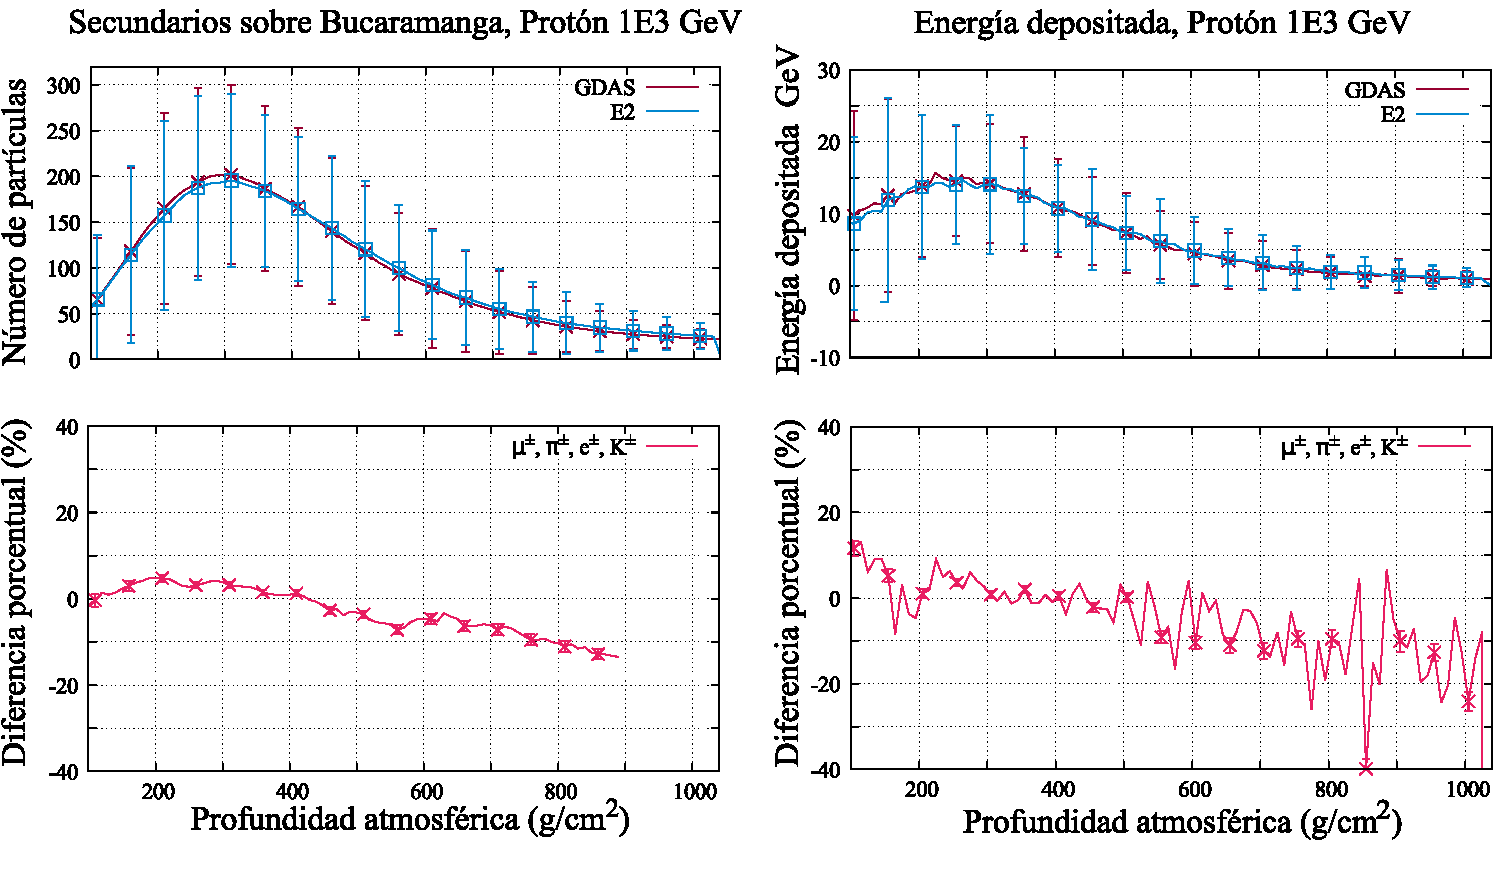
\includegraphics[width=0.8\textwidth]{Figs/proton_1E3.pdf}
\caption[Distribución longitudinal de un protón de $1\cdot 10^{3}$ GeV.]{Distribución longitudinal de un protón de $1\cdot 10^{3} GeV$ que fue simulado 5000 veces, usando la atmósfera predeterminada (línea azul), y usando la atmósfera construida para el mes de abril (línea roja).}
\label{fig:fig26}
\end{figure}

\begin{figure}[htb!]
\centering
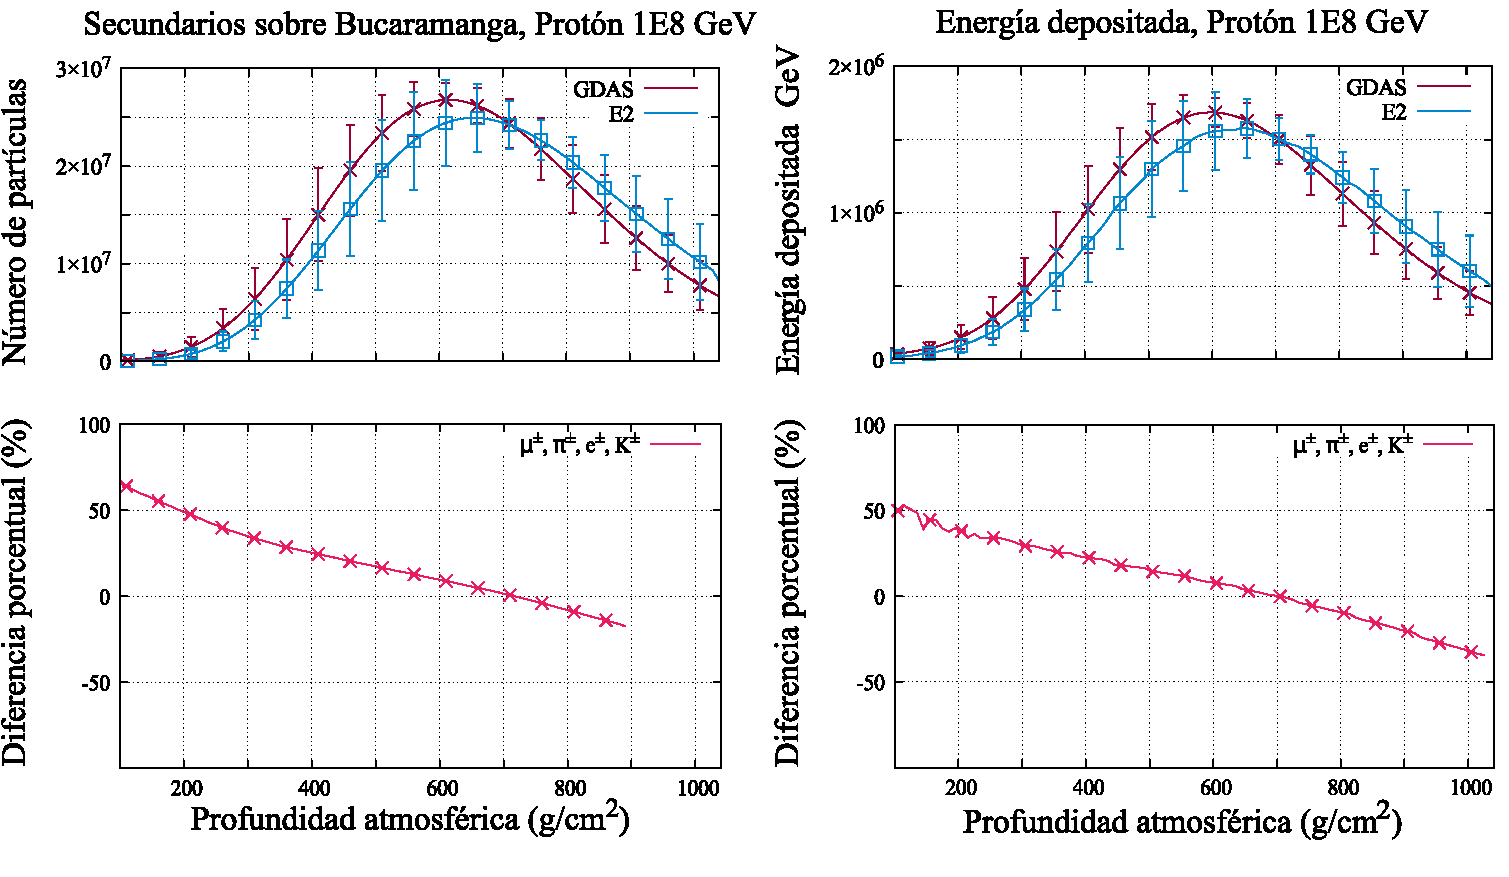
\includegraphics[width=0.8\textwidth]{Figs/proton_1E8.pdf}
\caption[Distribución longitudinal de un protón de $1\cdot 10^{8}$ GeV.]{Distribución longitudinal de un protón de $1\cdot 10^{8} GeV$ que fue simulado 10 veces, usando la atmósfera predeterminada (línea azul), y usando la atmósfera construida para el mes de abril (línea roja). }
\label{fig:fig26b}
\end{figure}


\begin{figure}[htb!]
\centering
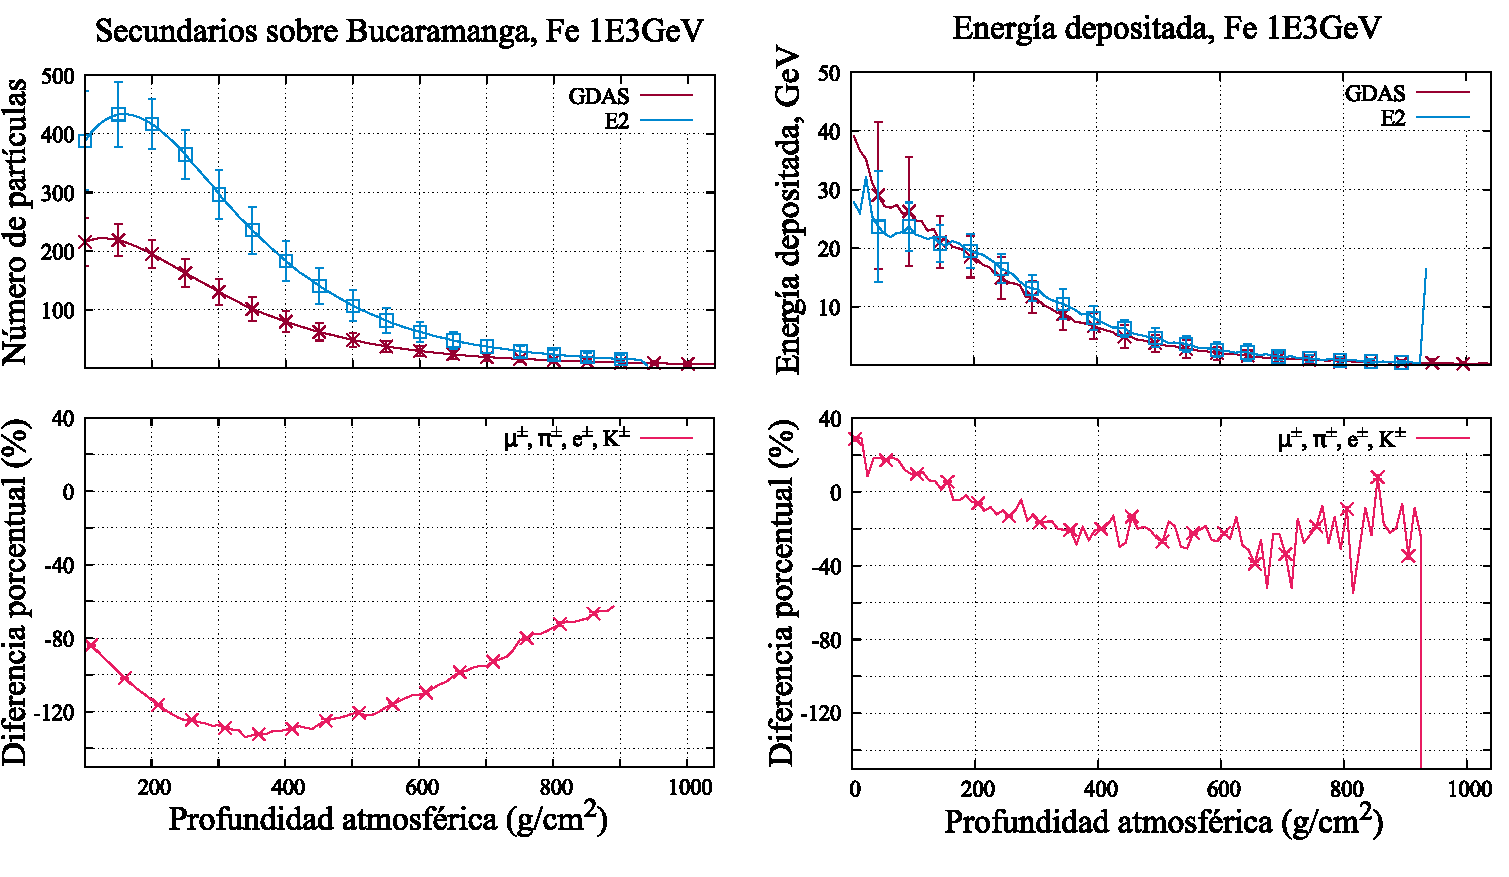
\includegraphics[width=0.8\textwidth]{Figs/fe_1E3.pdf}
\caption[Distribución longitudinal de un núcleo de hierro de $1\cdot 10^{3}$ GeV.]{Distribución longitudinal de un núcleo de hierro de $1\cdot 10^{3} GeV$ que fue simulado 5000 veces, usando la atmósfera predeterminada (línea azul), y usando la atmósfera construida para el mes de abril (línea roja). }
\label{fig:fig27}
\end{figure}

\begin{figure}[htb!]
\centering
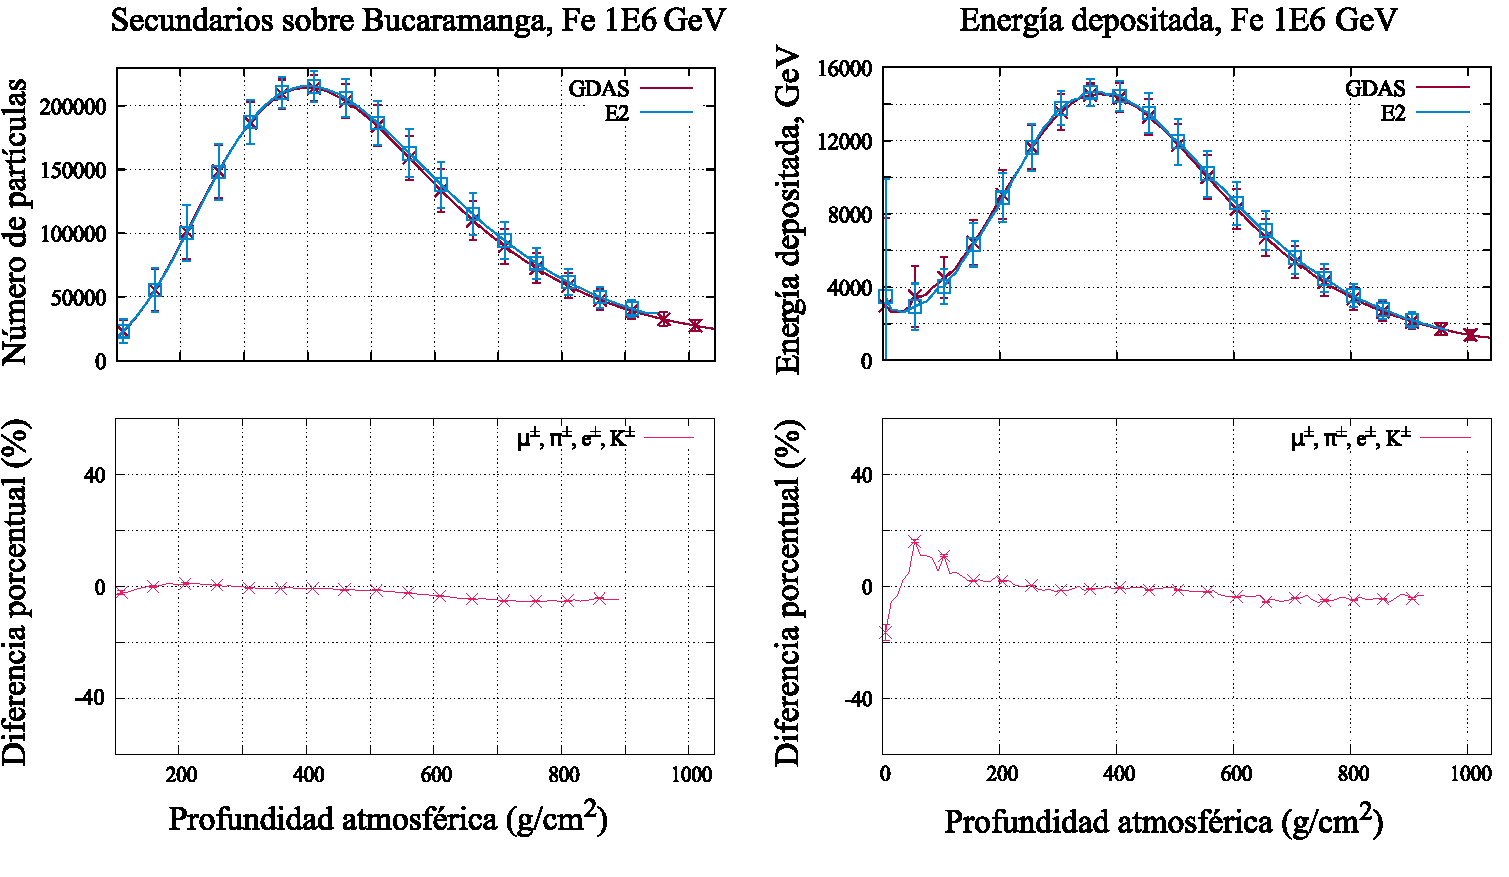
\includegraphics[width=0.8\textwidth]{Figs/fe_1E6.pdf}
\caption[Distribución longitudinal de un núcleo de hierro de $1\cdot 10^{6}$ GeV.]{Distribución longitudinal de un núcleo de hierro de $1\cdot 10^{6} GeV$ que fue simulado 1000 veces, usando la atmósfera predeterminada (línea azul), y usando la atmósfera construida para el mes de abril (línea roja). }
\label{fig:fig28}
\end{figure}

\begin{figure}[htb!]
\centering
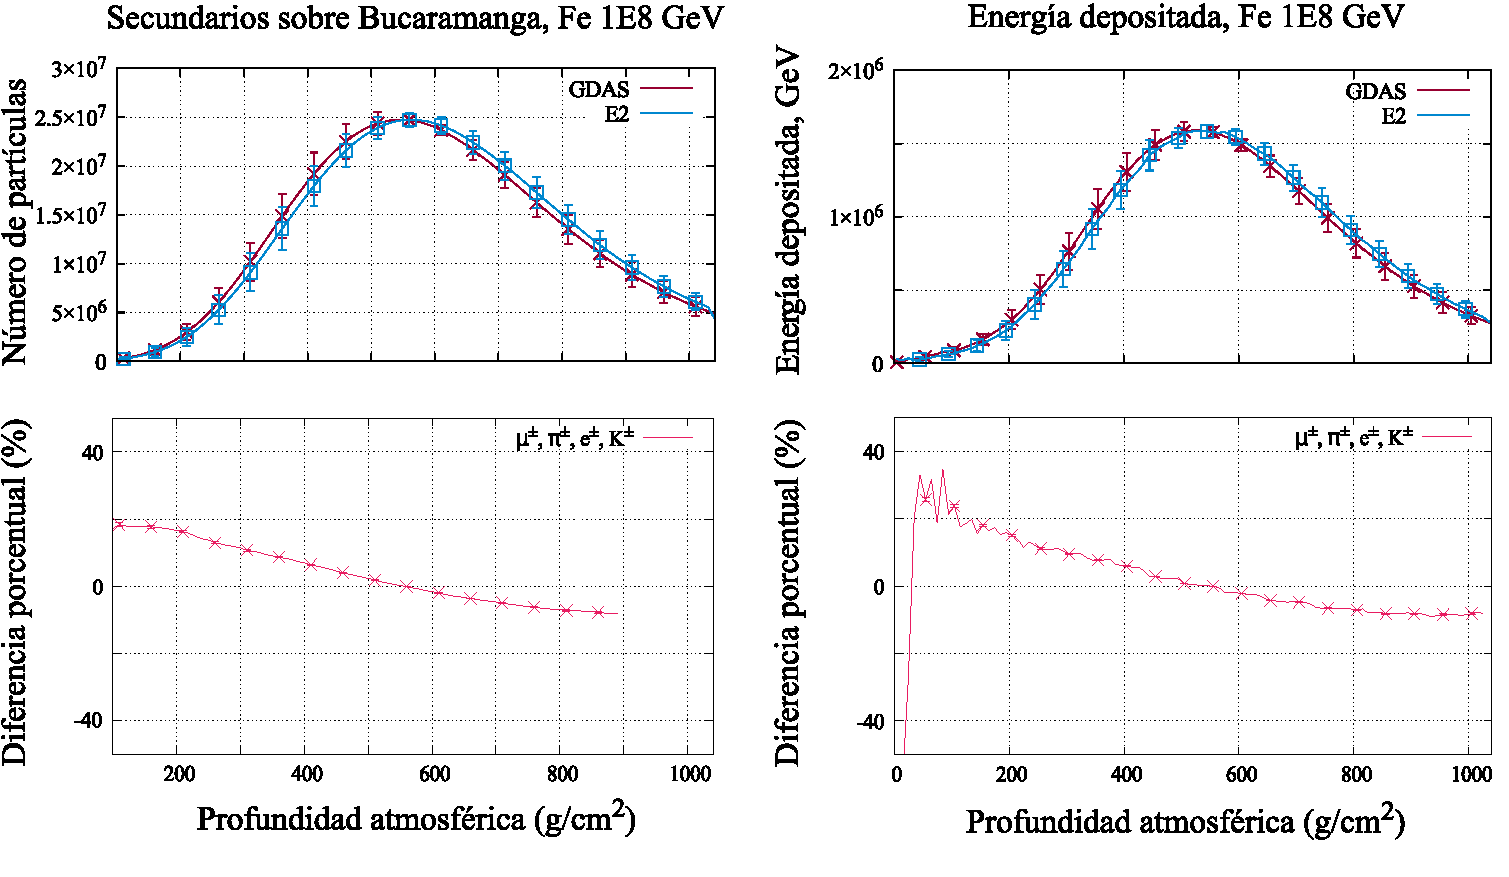
\includegraphics[width=0.8\textwidth]{Figs/fe_1E8.pdf}
\caption[Distribución longitudinal de un núcleo de hierro de $1\cdot 10^{8}$ GeV.]{Distribución longitudinal de un núcleo de hierro de $1\cdot 10^{3} GeV$ que fue simulado 10 veces, usando la atmósfera predeterminada (línea azul), y usando la atmósfera construida para el mes de abril (línea roja). }
\label{fig:fig29}
\end{figure}

\begin{figure}[htb!]
\centering
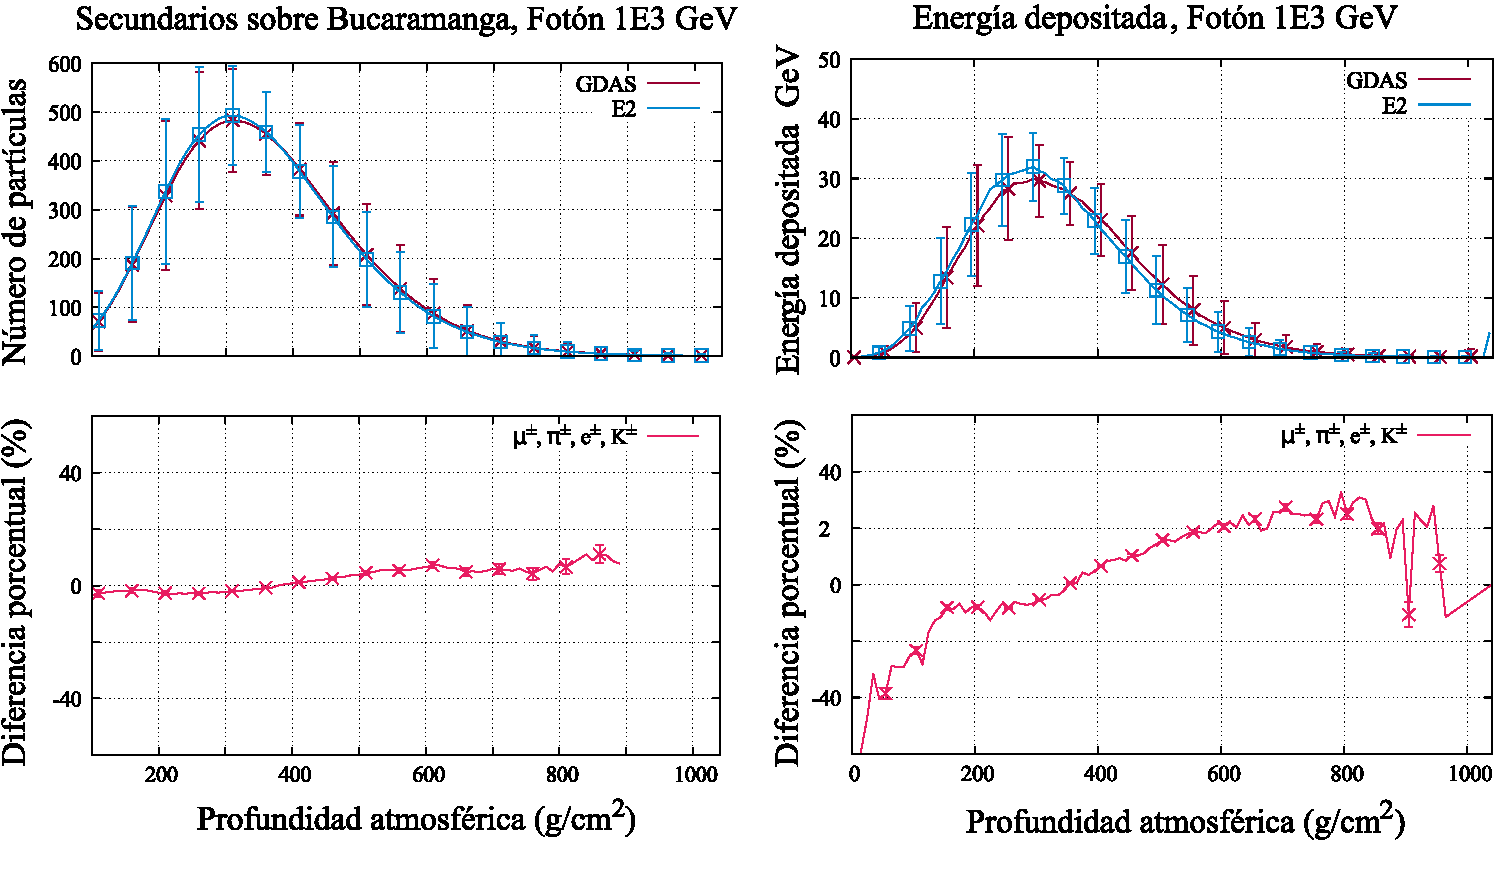
\includegraphics[width=0.8\textwidth]{Figs/foton_1E3.pdf}
\caption[Distribución longitudinal de un fotón de $1\cdot 10^{3}$ GeV.]{Distribución longitudinal de un foton de $1\cdot 10^{3} GeV$ que fue simulado 5000 veces, usando la atmósfera predeterminada (línea azul), y usando la atmósfera construida para el mes de abril (línea roja).}
\label{fig:fig30}
\end{figure}

\begin{figure}[htb!]
\centering
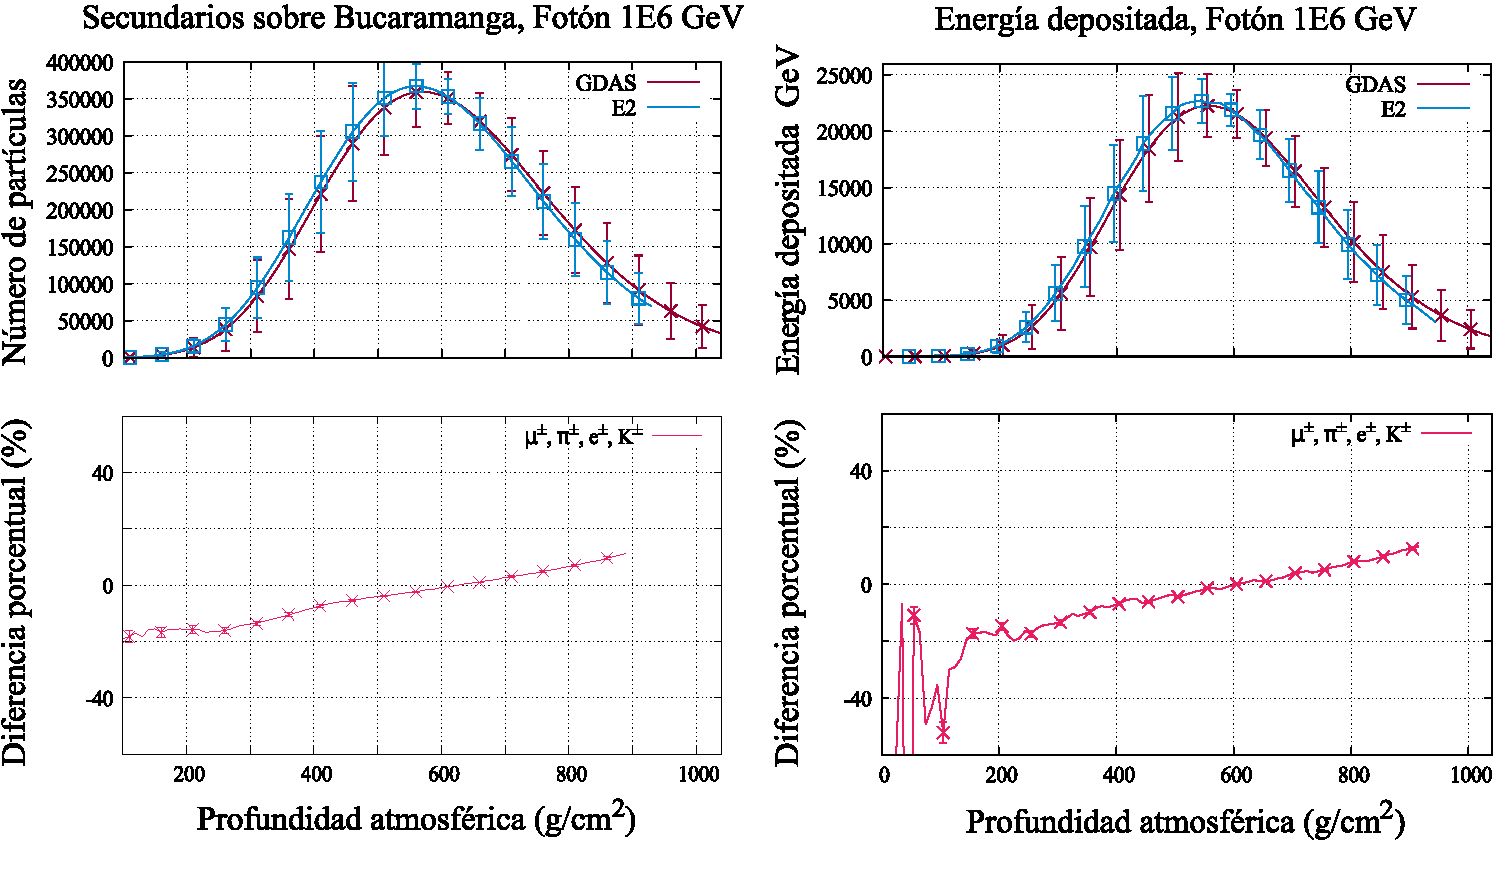
\includegraphics[width=0.8\textwidth]{Figs/foton_1E6.pdf}
\caption[Distribución longitudinal de un fotón de $1\cdot 10^{6}$ GeV.]{Distribución longitudinal de un fotón de $1\cdot 10^{6} GeV$ que fue simulado 1000 veces, usando la atmósfera predeterminada (línea azul), y usando la atmósfera construida para el mes de abril (línea roja). }
\label{fig:fig31}
\end{figure}

\begin{figure}[htb!]
\centering
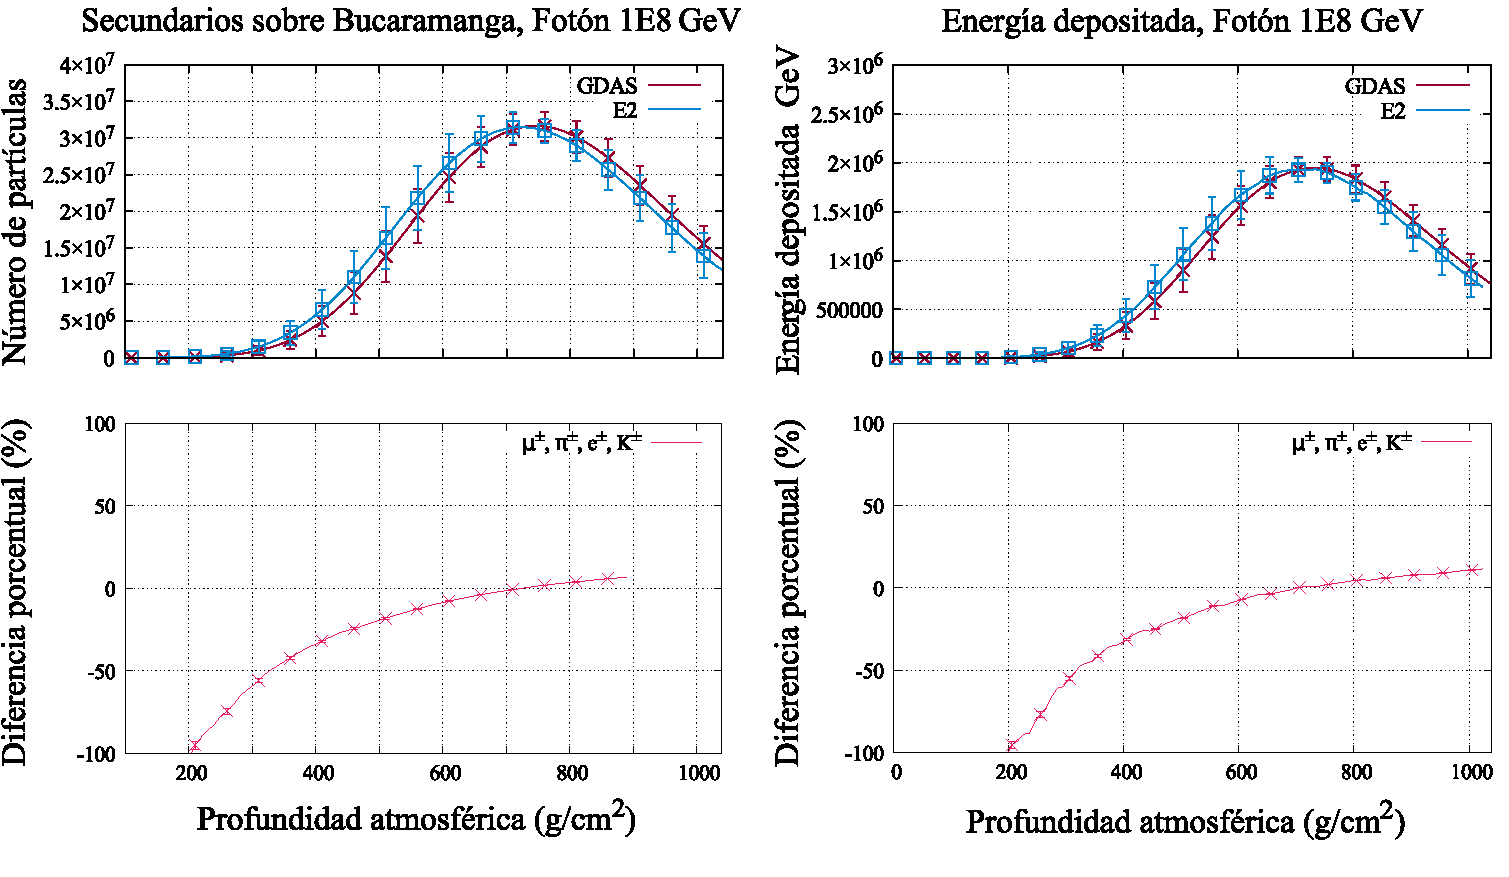
\includegraphics[width=0.8\textwidth]{Figs/foton_1E8.pdf}
\caption[Distribución longitudinal de un fotón de $1\cdot 10^{8}$ GeV.]{Distribución longitudinal de un fotón de $1\cdot 10^{8} GeV$ que fue simulado 10 veces, usando la atmósfera predeterminada (línea azul), y usando la atmósfera construida para el mes de abril (línea roja). }
\label{fig:fig32}
\end{figure}






% ------------------------------------------------------------------------
\end{document}                                          % Fin de documento
% ------------------------------------------------------------------------ 